\chapter{Implementierung}
\label{chap:implementierung}
Dieses Kapitel beschreibt die technische Realisierung des Prototyps. Es werden die Implementierungsdetails der in Kapitel \ref{chap:konzeption} konzipierten Architektur dargelegt, von der Datenaufbereitung über das Modelltraining bis zur finalen Datenaggregation.

\section{Technologiestack und Entwicklungsumgebung}

Die Implementierung des Prototyps basiert auf bewährten Open-Source-Technologien und -Bibliotheken. Die Auswahl des Technologiestacks erfolgte unter Berücksichtigung von Leistung, Wartbarkeit, Datenschutz und der Verfügbarkeit von Community-Support.

\subsection{Programmiersprache und Kernbibliotheken}

Die gesamte Implementierung erfolgte in \textbf{Python 3.9}, da diese Sprache ein umfangreiches Ökosystem für maschinelles Lernen, Bildverarbeitung und Datenmanipulation bietet und eine schnelle Prototypenentwicklung ermöglicht.

\begin{table}[H]
\centering
\small
\begin{tabular}{|l|l|l|p{7cm}|}
\hline
\textbf{Komponente} & \textbf{Bibliothek} & \textbf{Version} & \textbf{Einsatzzweck} \\
\hline
\multicolumn{4}{|c|}{\textit{Maschinelles Lernen}} \\
\hline
Deep Learning & PyTorch & 2.0.1 & Framework für neuronale Netze \\
Objekterkennung & Ultralytics & 8.0.196 & YOLOv8 Implementierung \\
OCR (primär) & PaddleOCR & 2.7.0 & Hauptengine für Texterkennung \\
OCR (Fallback 1) & Tesseract & 5.3.0 & Fallback für niedrig aufgelöste oder verrauschte Texte \\
OCR (Fallback 2) & EasyOCR & 1.7.0 & Optionale dritte Engine \\
\hline
\multicolumn{4}{|c|}{\textit{Bildverarbeitung}} \\
\hline
Bildmanipulation & OpenCV & 4.8.0 & Preprocessing, Transformationen \\
Bildoperationen & Pillow & 10.0.0 & Zusätzliche Bildoperationen \\
PDF-Verarbeitung & PyMuPDF & 1.23.3 & PDF-zu-Bild Konvertierung \\
\hline
\multicolumn{4}{|c|}{\textit{Datenverarbeitung}} \\
\hline
Numerik & NumPy & 1.24.3 & Array-Operationen, Mathematik \\
Datenstrukturen & Pandas & 2.0.3 & Tabellarische Datenmanipulation \\
\hline
\multicolumn{4}{|c|}{\textit{Benutzeroberfläche \& Persistenz}} \\
\hline
GUI-Framework & PyQt5 & 5.15.9 & Desktop-Anwendung \\
Datenbank & PostgreSQL & 14.9 & Datenpersistenz \\
ORM & psycopg2 & 2.9.7 & PostgreSQL-Adapter \\
\hline
\end{tabular}
\caption{Übersicht der verwendeten Technologien und Bibliotheken}
\label{tab:tech_stack}
\end{table}
\textbf{Lizenzkonformität (NFA-002):} Alle verwendeten Bibliotheken unterliegen 
Open-Source-Lizenzen (Apache 2.0, MIT, BSD), die für den kommerziellen Einsatz 
bei Siemens Mobility geeignet sind. Eine detaillierte Lizenzprüfung wurde durchgeführt 
und bestätigt die Konformität mit den Unternehmensrichtlinien.
\subsection{Entwicklungsumgebung}
Die Entwicklung erfolgte in Visual Studio Code mit Git-Versionskontrolle. 
Die Annotation wurde mittels CVAT (Version 2.5.0) in lokaler Docker-Umgebung 
durchgeführt \cite{cvat}. Abhängigkeiten sind in \texttt{requirements.txt} dokumentiert.


\subsection{Hardware-Infrastruktur}

Das YOLOv8-Training erfolgte auf einer GPU-Instanz (NVIDIA, AWS Instance g4dn.xlarge, 16 GB VRAM). Die finale Anwendung ist CPU-kompatibel (Intel Core i7, 32 GB RAM), um eine breite Einsetzbarkeit ohne spezialisierte Hardware zu gewährleisten.

\subsection{Projektstruktur}

Die Implementierung folgt einer modularen Architektur mit klarer Trennung der Verantwortlichkeiten:

\begin{itemize}
    \item \texttt{core/} - Kernlogik der Pipeline
    \begin{itemize}
        \item \texttt{detection.py} - YOLO Objekterkennung
        \item \texttt{ocr.py} - OCR-Engine Wrapper
        \item \texttt{linking.py} - Symbol-Text Verknüpfung
    \end{itemize}
    \item \texttt{ui/} - PyQt5 Benutzeroberfläche
    \item \texttt{utils/} - Hilfsfunktionen
    \item \texttt{validation/} - Validierungsregeln
    \item \texttt{database.py} - Datenbankzugriff
    \item \texttt{main.py} - Haupteinstiegspunkt
\end{itemize}

\textbf{Modularität (FA-014, NFA-008):} Die dargestellte Projektstruktur gewährleistet 
eine klare Trennung der Verantwortlichkeiten. Jedes Modul (\texttt{core/}, \texttt{ui/}, 
\texttt{validation/}) kann unabhängig weiterentwickelt werden. Die Integration neuer 
Symbolklassen erfordert lediglich Anpassungen in \texttt{core/detection.py} und 
\texttt{core/linking.py}, ohne die UI- oder Export-Logik zu modifizieren.

\section{Objekterkennung mit YOLOv8-OBB}
\label{sec:objekterkennungmityolov8obb}
Die Objekterkennung bildet die erste und fundamentale Stufe der Extraktionspipeline. Ihre Aufgabe besteht darin, alle relevanten Symbole in den Gleisplänen zu lokalisieren und zu klassifizieren. Die Qualität dieser Detektionen bestimmt maßgeblich die Leistungsfähigkeit der nachfolgenden OCR- und Verknüpfungsmodule. Die Wahl fiel auf YOLOv8 in der Oriented Bounding Box (OBB) Variante, da diese Architektur speziell für die Detektion rotierter Objekte konzipiert wurde und somit optimal für technische Zeichnungen mit beliebig orientierten Symbolen geeignet ist.

\subsection{Datensatzerstellung und Annotation}
\label{subsec:Datensatzerstellung}
Die Leistungsfähigkeit eines objekterkennenden Modells hängt direkt von der Qualität und Quantität des Trainingsdatensatzes ab. Die Erstellung des Datensatzes erfolgte in einem mehrstufigen Prozess, der sowohl die Vorverarbeitung der Rohdaten als auch die präzise Annotation der Symbole umfasste.

\subsubsection{Vorverarbeitung der Gleispläne}

Die initialen Gleispläne lagen im PDF-Format vor und mussten zunächst in ein für die Annotation geeignetes Bildformat überführt werden. Hierzu wurde die Python-Bibliothek PyMuPDF eingesetzt, welche eine zuverlässige Rasterisierung von PDF-Dokumenten ermöglicht. Die Konvertierung erfolgte mit einer Auflösung von 500 DPI (dots per inch), was einem Skalierungsfaktor von $\frac{500}{72} \approx 6.94$ gegenüber der Standard-PDF-Auflösung entspricht. Diese hohe Auflösung wurde gewählt, um auch kleine Symbole wie Gleiskoppelspulenplatten oder Isolierstöße mit ausreichender Detailgenauigkeit darzustellen.

Nach der Rasterisierung wurden die hochauflösenden Bilder in kleinere, überlappende Bildausschnitte segmentiert. Die gewählte Segmentgröße für die Annotation und das Training betrug $1024 \times 1024$ Pixel, entsprechend der YOLO-Eingabegröße. Für die Inferenz werden größere Tiles ($2048 \times 2048$ Pixel) verwendet und vor der Modellverarbeitung auf $1024 \times 1024$ Pixel herunterskaliert (siehe Abschnitt~\ref{Inferenz}). Diese Dimensionierung stellt einen Kompromiss dar zwischen ausreichendem Kontext für die Objekterkennung und der effizienten Verarbeitung auf GPU-Systemen mit begrenztem Videospeicher. Größere Tiles würden zwar mehr Kontext bieten, jedoch den verfügbaren VRAM der Trainings-GPU (NVIDIA, AWS Instance g4dn.xlarge, 16 GB VRAM) überschreiten und damit das Training unmöglich machen oder die Batch-Größe unzulässig reduzieren.

\subsubsection{Annotationsprozess}

Die Beschriftung erfolgte mittels CVAT \cite{cvat} in lokaler Docker-Umgebung. 
Jedes Symbol wurde mit einer Oriented Bounding Box (OBB) annotiert (vgl. 
Abschnitt \ref{sec:orientedboundingboxesalslösung}), repräsentiert durch Zentrum $(c_x, c_y)$, Dimensionen 
$(w, h)$ und Rotationswinkel $\theta$:

$$\text{OBB} = (c_x, c_y, w, h, \theta)$$

CVAT exportiert im YOLO-OBB-Format mit normalisierten Eckpunktkoordinaten 
$\{(x_i/W, y_i/H)\}_{i=1}^{4}$.

\subsubsection{Datenaufteilung und Statistiken}

Der finale Datensatz umfasst insgesamt 13 Symbolklassen, darunter Signale, verschiedene Weichentypen, Koordinatenbeschriftungen, Haltepunkte, Isolierstöße und weitere eisenbahnspezifische Elemente. Die Daten wurden in einen Validierungssatz mit 115 Bildern und 1.305 annotierten Objektinstanzen aufgeteilt. Der Trainingssatz umfasste entsprechend die verbliebenen Bilder.

Die Verteilung der Objektinstanzen über die Klassen hinweg zeigt Tabelle \ref{tab:dataset_distribution}:

\begin{table}[H]
\centering
\begin{tabular}{|l|r|r|}
\hline
\textbf{Klasse} & \textbf{Bilder} & \textbf{Instanzen} \\
\hline
\multicolumn{3}{|c|}{\textit{Kernklassen (produktionsrelevant)}} \\
\hline
coordinate & 113 & 629 \\
signal & 81 & 218 \\
gks\_gesteuert & 67 & 69 \\
gm\_block & 55 & 91 \\
gks\_festkodiert & 43 & 60 \\
\hline
\textbf{Summe Kernklassen} & --- & \textbf{1.067 (81.8\%)} \\
\hline
\multicolumn{3}{|c|}{\textit{Auxiliarklassen (Erweiterbarkeit)}} \\
\hline
sverbinder & 81 & 85 \\
haltepunkt & 47 & 47 \\
weichen\_block & 25 & 39 \\
isolierstoß & 16 & 27 \\
prellblock & 14 & 16 \\
haltetafel & 11 & 11 \\
weichengruppeende & 9 & 9 \\
endeweichen & 4 & 4 \\
\hline
\textbf{Summe Auxiliarklassen} & --- & \textbf{238 (18.2\%)} \\
\hline
\hline
\textbf{Gesamt} & \textbf{115} & \textbf{1.305} \\
\hline
\end{tabular}
\caption{Verteilung der Annotationen über Klassen und Bilder im Validierungssatz, unterteilt nach Kern- und Auxiliarklassen (vgl. Anforderung FA-003)}
\label{tab:dataset_distribution}
\end{table}

Es ist ersichtlich, dass die Klassenverteilung unausgeglichen ist, mit Koordinaten und Signalen als dominierende Klassen. Diese Verteilung spiegelt die reale Häufigkeit der Symbole in Gleisplänen wider. Um ein Overfitting auf häufige Klassen zu vermeiden, wurde während des Trainings eine klassengewichtete Verlustfunktion zwar in Betracht gezogen, letztendlich jedoch zugunsten einer robusten Datenaugmentation verworfen.
\textbf{Klassenpriorisierung:} Gemäß Anforderung \textbf{FA-003} werden die Objektklassen 
in zwei Kategorien unterteilt. Die fünf \textit{Kernklassen} (signal, coordinate, 
gks\_festkodiert, gks\_gesteuert, gm\_block) repräsentieren die für die Projektierung 
bei Siemens Mobility essentiellen Symbole und bilden den Fokus der End-to-End-Evaluation 
in Kapitel~\ref{chap:evaluation}. Die acht \textit{Auxiliarklassen} wurden zusätzlich 
implementiert, um die Erweiterbarkeit des Systems zu demonstrieren (vgl. Anforderung 
\textbf{NFA-008}), werden jedoch nicht im Detail evaluiert.
Die Daten wurden in eine standardisierte COCO-Verzeichnisstruktur (Abbildung \ref{fig:COCODatenset}) überführt, welche die Organisation von Trainings- und Validierungsdaten sowie die zugehörigen Annotationen in separaten Verzeichnissen vorsieht.

\begin{figure}[H]
    \centering
    \includegraphics[width=5cm]{images/Kapitel6/cocodatasetconfig.png} 
    \caption{COCO-konforme Datensetstruktur für YOLOv8-OBB Training}
    \label{fig:COCODatenset}
\end{figure}

\begin{figure}[H]
    \centering
    \includegraphics[width=0.95\textwidth]{images/Kapitel7/labels.jpg}
    \caption{Charakteristika des Trainingsdatensatzes: (oben links) Klassenverteilung mit absoluten Instanzzahlen, (unten links) räumliche Verteilung der Bounding-Box-Zentren, (unten rechts) Größenverteilung der annotierten Objekte in normalisierten Koordinaten.}
    \label{fig:labels_distribution}
\end{figure}
Abbildung~\ref{fig:labels_distribution} visualisiert die Charakteristika des annotierten Trainingsdatensatzes. Die Klassenverteilung zeigt eine deutliche Dominanz der Koordinaten-Klasse (5.945 Instanzen), gefolgt von Signalen (1.875 Instanzen). Diese Ungleichverteilung spiegelt die tatsächliche Häufigkeit der Symbole in realen Gleisplänen wider und wurde bewusst beibehalten, um das Modell auf praxisnahe Verteilungen zu trainieren. Die räumliche Verteilung der Bounding-Box-Zentren zeigt eine gleichmäßige Abdeckung des Bildbereichs, während die Größenverteilung die charakteristisch kleinen Objektgrößen der Gleisplansymbole verdeutlicht.
\subsubsection{Synthetische Datenaugmentation durch Rotation}

Um die Robustheit des Modells gegenüber beliebigen Symbolorientierungen zu verbessern und die Klassenbalance zu optimieren, wurde eine gezielte synthetische Augmentation durch Rotation implementiert. Diese Strategie adressiert zwei zentrale Herausforderungen:

\begin{enumerate}
    \item \textbf{Klassenungleichgewicht}: Die natürliche Verteilung der Symbolklassen im Datensatz ist stark unausgeglichen (vgl. Tabelle~\ref{tab:dataset_distribution}), mit dominierenden Klassen wie \textit{coordinate} (629 Instanzen) und unterrepräsentierten Klassen wie \textit{endeweichen} (4 Instanzen).
    
    \item \textbf{Orientierungsvielfalt}: Obwohl technische Zeichnungen Symbole in verschiedenen Winkeln enthalten, sind bestimmte Orientierungen (insbesondere $0^\circ$ und $90^\circ$) überrepräsentiert, während diagonale Ausrichtungen seltener auftreten.
\end{enumerate}

\textbf{Augmentationsstrategie:}

Die synthetische Rotation wurde selektiv auf unterrepräsentierte Klassen angewendet. Für jede Instanz einer Zielklasse wurden systematische Rotationen um folgende Winkel durchgeführt:

$$\Theta_{\text{aug}} = \{-90^\circ, -60^\circ, -45^\circ, -30^\circ, -15^\circ, +15^\circ, +30^\circ, +45^\circ, +60^\circ, +90^\circ\}$$

Die Rotation erfolgte um den Zentroid $(c_x, c_y)$ der Oriented Bounding Box, wobei sowohl die Bildregion als auch die OBB-Koordinaten entsprechend transformiert wurden. Die Rotationsmatrix für einen Winkel $\theta$ lautet:

$$\mathbf{R}(\theta) = \begin{pmatrix} 
\cos(\theta) & -\sin(\theta) \\ 
\sin(\theta) & \cos(\theta) 
\end{pmatrix}$$

\textbf{Rotationsinvarianz (FA-002):} Die synthetische Augmentation mit 10 
Rotationswinkeln ($\Theta_{\text{aug}} = \{-90^\circ, -60^\circ, ..., +90^\circ\}$) stellt sicher, 
dass das Modell Symbole in beliebigen Orientierungen erkennen kann. In Kombination 
mit der OBB-Architektur wird eine vollständige Rotationsinvarianz von $0^\circ$ bis $360^\circ$ 
erreicht.


\textbf{Klassenspezifische Augmentation:}

Die Anzahl der generierten synthetischen Samples wurde klassenabhängig gesteuert, um eine Zielverteilung von ca. 600 Instanzen pro Klasse zu erreichen (Ausnahme: \textit{coordinate} mit Ziel +300 Instanzen aufgrund der bereits hohen Ausgangsanzahl).

\begin{table}[H]
\centering
\small
\begin{tabular}{|l|r|r|r|r|}
\hline
\textbf{Klasse} & \textbf{Original} & \textbf{Augmentiert} & \textbf{Gesamt} & \textbf{Faktor} \\
\hline
\multicolumn{5}{|c|}{\textit{Kernklassen}} \\
\hline
coordinate & 629 & 300 & 929 & 1.48x\\
signal & 218 & 382 & 600 & 2.75x \\
gks\_gesteuert & 69 & 531 & 600 & 8.70x \\
gm\_block & 91 & 509 & 600 & 6.59x \\
gks\_festkodiert & 60 & 540 & 600 & 10.00x \\
\hline
\textbf{Summe Kernklassen} & \textbf{1.067} & \textbf{2.262} & \textbf{3.329} & --- \\
\hline
\multicolumn{5}{|c|}{\textit{Auxiliarklassen}} \\
\hline
sverbinder & 85 & 515 & 600 & 7.06x\\
haltepunkt & 47 & 553 & 600 & 12.77x\\
weichen\_block & 39 & 561 & 600 & 15.38x\\
isolierstoß & 27 & 573 & 600 & 22.22x \\
prellblock & 16 & 584 & 600 & 37.50x \\
haltetafel & 11 & 589 & 600 & 54.55x \\
endeweichen & 4 & 596 & 600 & 150.00x \\
weichengruppeende & 9 & 591 & 600 & 66.67x \\
\hline
\textbf{Summe Auxiliarklassen} & \textbf{238} & \textbf{4.462} & \textbf{4.700} & --- \\
\hline
\hline
\textbf{Gesamt} & \textbf{1.305} & \textbf{6.724} & \textbf{8.029} & \textbf{6.15x} \\
\hline
\end{tabular}
\caption{Verteilung der Instanzen vor und nach synthetischer Rotation, unterteilt nach Kern- und Auxiliarklassen}
\label{tab:augmentation_statistics}
\end{table}

\textbf{Technische Umsetzung:}
Die hohen Augmentationsfaktoren für seltene Klassen (z.B. 150x für \textit{endeweichen}) sind gerechtfertigt, da diese Symbole in realen Gleisplänen tatsächlich sehr selten vorkommen, das Modell aber dennoch in der Lage sein muss, sie zuverlässig zu erkennen. Die synthetische Rotation simuliert realistische Orientierungsvariationen und verhindert Overfitting auf die wenigen Original-Samples. 

Die finale Datensatzaufteilung erfolgte automatisch durch YOLOv8s integrierte Split-Funktion mit einem 80/20-Verhältnis, was zu 923 Trainings- und 208 Validierungsbildern führte. Nach manueller Filterung leerer oder irrelevanter Tiles verblieben 115 Validierungsbilder (1.305 Instanzen), die als dedizierter Testdatensatz für die Evaluation in Kapitel~\ref{chap:evaluation} dienen.
Die Rotation wurde in einem Preprocessing-Schritt vor dem Training durchgeführt und die augmentierten Samples wurden als separate Einträge im Trainingsdatensatz gespeichert. Dies ermöglicht eine deterministische Reproduzierbarkeit der Augmentation. Die Implementation erfolgte mittels OpenCV's \texttt{cv2.getRotationMatrix2D()} und \texttt{cv2.warpAffine()}, wobei die Bildgröße dynamisch angepasst wurde, um ein Abschneiden rotierter Objekte zu vermeiden.

\textbf{Validierung der Augmentation:}

Um sicherzustellen, dass die synthetische Rotation keine Artefakte einführt, wurden die augmentierten Samples manuell gesichtet. Die OBB-Annotationen wurden entsprechend transformiert und auf geometrische Korrektheit geprüft.
\subsection{Modelltraining und Optimierung}
\label{subsec:Modelltraining}
Das Training des YOLOv8-OBB Modells wurde auf einer cloud-basierten GPU-Instanz mit einer NVIDIA AWS Instance g4dn.xlarge, (16 GB VRAM) durchgeführt. Die Wahl einer externen GPU-Instanz war notwendig, da lokale Entwicklungsmaschinen nicht über ausreichende Rechenleistung verfügen, um das Training in angemessener Zeit abzuschließen.

\subsubsection{Modellarchitektur und Hyperparameter}

Als Basismodell wurde YOLOv8l-OBB gewählt, die \enquote{Large}-Variante von YOLOv8 mit OBB-Unterstützung. Diese Modellgröße stellt eine Balance zwischen Detektionspräzision und Inferenzgeschwindigkeit dar. Kleinere Varianten (YOLOv8n, YOLOv8s) wären zwar schneller, zeigen jedoch bei komplexen Szenen mit kleinen Objekten deutliche Leistungseinbußen. Größere Varianten (YOLOv8x) würden nur marginale Verbesserungen bringen, bei gleichzeitig erheblich längerer Trainings- und Inferenzzeit.

Die vollständige Konfiguration der Trainingsparameter ist in Tabelle \ref{tab:yolo_training_params} dargestellt:

\begin{table}[H]
\centering
\begin{tabular}{|l|r|p{6cm}|}
\hline
\textbf{Parameter} & \textbf{Wert} & \textbf{Begründung} \\
\hline
Modellgröße & YOLOv8l-OBB & Balance zwischen Präzision und Inferenzgeschwindigkeit \\
Eingabeauflösung & $1024 \times 1024$ & Angepasst an Tile-Größe der Annotationen \\
Epochen & 120 & Ausreichend für vollständige Konvergenz ohne Overfitting \\
Batch Size & 6 & Maximal mögliche Größe bei 16 GB VRAM der T4 GPU \\
Optimizer & SGD & Momentum = 0.937, Weight Decay = 0.0005 \\
Learning Rate & 0.01 & Initiale LR mit Cosine Annealing Scheduler \\
Warmup Epochs & 3 & Graduelle Erhöhung der LR zu Trainingsbeginn \\
Workers & 2 & Moderat gewählt zur Vermeidung von Speicherüberläufen (Out of Memory) im Dataloader \\
Cache & Disk & Disk-Caching für deterministische Reproduzierbarkeit \\
Seed & 0 & Fixierter Seed für vollständige Reproduzierbarkeit \\
\hline
\end{tabular}
\caption{YOLOv8-OBB Trainingsparameter}
\label{tab:yolo_training_params}
\end{table}

Die Batch-Größe von 6 wurde empirisch durch schrittweise Erhöhung ermittelt, bis die GPU-Speichergrenze erreicht wurde. Eine größere Batch-Größe würde zwar stabilere Gradienten liefern, ist jedoch durch die Hardware-Limitierung nicht realisierbar.

Der Stochastic Gradient Descent (SGD) Optimizer wurde gegenüber adaptiven Optimierern wie Adam bevorzugt, da SGD in der Regel zu Modellen mit besserer Generalisierungsfähigkeit führt, auch wenn die Konvergenz langsamer verläuft. Der Momentum-Term von 0.937 beschleunigt die Konvergenz in relevanten Richtungen und dämpft Oszillationen.

Die Learning Rate wurde mittels Cosine Annealing Scheduler von einem initialen Wert von 0.01 graduell auf nahezu 0 reduziert. Diese Strategie ermöglicht zu Beginn des Trainings große Schritte im Parameterraum und verfeinert gegen Ende die Gewichte durch immer kleinere Anpassungen.

\subsubsection{Datenaugmentation}

Um die Robustheit des Modells gegenüber Variationen in den Eingangsdaten zu erhöhen und Overfitting zu vermeiden, wurden verschiedene Augmentierungstechniken angewendet. Die Konfiguration der Augmentierungsparameter zeigt Tabelle \ref{tab:augmentation}:

\begin{table}[H]
\centering
\begin{tabular}{|l|r|p{7cm}|}
\hline
\textbf{Augmentation} & \textbf{Parameter} & \textbf{Beschreibung} \\
\hline
Rotation & $0.0^\circ$ & Deaktiviert, da OBB bereits Rotationsinvarianz bietet \\
Translation & $\pm 5\%$ & Horizontale und vertikale Verschiebung um bis zu 5\% der Bildgröße \\
Skalierung & $\pm 20\%$ & Zufällige Vergrößerung oder Verkleinerung um bis zu 20\% \\
Scherung & $0.0^\circ$ & Deaktiviert, um geometrische Integrität zu bewahren \\
Perspektive & 0.0 & Deaktiviert aus gleichem Grund \\
Horizontal Flip & 20\% & Spiegelung mit 20\% Wahrscheinlichkeit \\
Vertical Flip & 0\% & Deaktiviert, da vertikale Orientierung semantisch relevant ist \\
Mosaic & 40\% & Kombination von 4 Bildern, deaktiviert ab Epoch 110 \\
Mixup & 10\% & Lineare Überlagerung zweier Bilder mit 10\% Wahrscheinlichkeit \\
\hline
\end{tabular}
\caption{Datenaugmentierungsparameter}
\label{tab:augmentation}
\end{table}

Die Deaktivierung der Rotationsaugmentation mag zunächst kontraintuitiv erscheinen, da die OBB-Architektur explizit für rotierte Objekte entwickelt wurde. Jedoch sind die Rotationswinkel der Symbole bereits in den OBB-Annotationen kodiert, sodass eine zusätzliche künstliche Rotation redundant wäre. Stattdessen lernt das Modell, die Orientierung direkt aus den rotierten Bounding Boxes zu extrahieren.

Die Mosaic-Augmentation kombiniert vier zufällig ausgewählte Trainingsbilder zu einem neuen Bild, indem sie in einem 2x2-Raster angeordnet werden. Diese Technik zwingt das Modell, Objekte auch in ungewöhnlichen Kontexten und bei veränderten Größenverhältnissen zu erkennen. Die Deaktivierung der Mosaic-Augmentation in den letzten 10 Epochen (close\_mosaic = 10) ermöglicht dem Modell, sich in der Feinabstimmungsphase auf realistische, unveränderte Bilder zu fokussieren.

Die Trainingsdauer betrug insgesamt ca. 8 Stunden bei kontinuierlicher GPU-Auslastung von nahezu 100\%.

\subsubsection{Trainingsergebnisse}

Das Training wurde über 120 Epochen durchgeführt und erreichte eine stabile Konvergenz 
ohne Anzeichen von Overfitting. Die Trainingsverläufe (Abbildung \ref{fig:yolo_training_curves}) 
illustrieren die Entwicklung der Verlustfunktionen über den Trainingsverlauf.

\begin{figure}[H]
\centering
\includegraphics[width=\textwidth]{images/Kapitel6/results.png}
\caption{Trainings- und Validierungsmetriken über 120 Epochen. Die Kurven zeigen eine 
stabile Konvergenz ohne Anzeichen von Overfitting.}
\label{fig:yolo_training_curves}
\end{figure}

Folgende Beobachtungen lassen sich aus den Kurven ableiten:

\begin{itemize}
    \item Die Box-Loss-Kurve fällt kontinuierlich und stabilisiert sich nach ca. 80 Epochen 
    auf einem niedrigen Niveau, was auf eine erfolgreiche Lokalisierungsoptimierung hindeutet.
    
    \item Die Classification-Loss-Kurve zeigt einen ähnlichen Verlauf, was die erfolgreiche 
    Konvergenz der Klassifikation belegt.
    
    \item Kritisch ist die Beobachtung, dass zwischen Trainings- und Validierungskurven 
    kein signifikanter Gap existiert. Dies belegt, dass das Modell gut generalisiert und 
    nicht auf den Trainingsdaten overfittet.
\end{itemize}
\textbf{Update-Fähigkeit (NFA-009):} Die trainierten Modellgewichte werden als 
externe Datei (\texttt{best.pt}) gespeichert und können ohne Code-Änderungen 
ausgetauscht werden. Bei Bedarf an neuen Symbolklassen kann ein Nachtraining 
(Fine-Tuning) auf dem bestehenden Modell durchgeführt werden.
Die detaillierte quantitative Auswertung der Detektionsleistung sowie die Analyse der 
Konfusionsmatrix erfolgen in Kapitel \ref{chap:evaluation}.

\subsection{Inferenz-Pipeline Implementierung}
\label{Inferenz}
Nach Abschluss des Trainings wurde das Modell mit den optimalen Gewichten (\texttt{best.pt}) in die produktive Extraktionspipeline integriert. Die Inferenz auf neuen, zuvor ungesehenen Gleisplänen erfolgt in mehreren aufeinander aufbauenden Schritten. Abbildung \ref{fig:pipeline_flowchart} zeigt den vollständigen Ablauf der Inferenz-Pipeline von der PDF-Eingabe über das Tiling bis zur Rücktransformation der globalen Koordinaten.
\begin{figure}[H]
    \centering
    \begin{tikzpicture}[
        node distance=0.8cm, % Abstand zwischen den Boxen
        font=\small,
        % --- STYLES ---
        % 1. Prozess-Schritte (Rechtecke)
        process/.style={
            rectangle, 
            draw=blue!60!black, 
            fill=blue!5, 
            text width=4cm, 
            align=center, 
            minimum height=1cm,
            rounded corners=2pt,
            thick,
            drop shadow % Schatten für Tiefe
        },
        % 2. Input/Output Daten (Trapeze oder andere Farbe)
        data/.style={
            rectangle,
            draw=gray!60!black,
            fill=gray!10,
            text width=3.5cm,
            align=center,
            minimum height=0.8cm,
            dashed, % Gestrichelt für Dateien/Daten
            thick
        },
        % 3. Parameter-Notiz
        note/.style={
            rectangle, 
            draw=none, 
            fill=yellow!10, 
            text width=3.5cm, 
            align=left, 
            font=\footnotesize
        },
        % 4. Pfeile
        arrow/.style={
            -Stealth, % Moderne Pfeilspitze
            thick,
            draw=black!80
        }
    ]

    % --- KNOTEN ---
    
    % Input
    \node[data] (pdf) {\textbf{Input:}\\Gleisplan};

    % Schritte
    \node[process, below=of pdf] (raster) {Rasterisierung\\(Rendering @ 500 DPI)};
    
    \node[process, below=of raster] (tile) {Tiling / Slicing\\($2048 \times 2048$ px)};
    
    \node[process, below=of tile, fill=green!10, draw=green!60!black] (yolo) {\textbf{YOLO Inferenz}\\(Objekterkennung)};
    
    \node[process, below=of yolo] (coord) {Koordinaten-\\Rücktransformation};
    
    \node[process, below=of coord] (nms) {Post-Processing\\(NMS \& Filterung)};

    % Output
    \node[data, below=of nms] (out) {\textbf{Output:}\\Strukturierte Detektionsliste\\(JSON / DataFrame)};

    % --- PFEILE ---
    \draw[arrow] (pdf) -- (raster);
    \draw[arrow] (raster) -- (tile);
    \draw[arrow] (tile) -- (yolo);
    \draw[arrow] (yolo) -- (coord);
    \draw[arrow] (coord) -- (nms);
    \draw[arrow] (nms) -- (out);

    % --- ANNOTATIONEN (Seitlich) ---
    % Verbindungslinie zu Tiling
    \node[note, right=1cm of tile] (tilingparams) {
        \textbf{Parameter:}\\
        $\bullet$ Stride: 1792 px\\
        $\bullet$ Halo: 128 px\\
        $\bullet$ Overlap: $\sim$12.5\%
    };
    \draw[dashed, gray] (tile) -- (tilingparams);

    \end{tikzpicture}
    \caption{Ablauf der Inferenz-Pipeline}
    \label{fig:pipeline_flowchart}
\end{figure}

\FloatBarrier
\subsubsection{Eingabeverarbeitung und Formatnormalisierung}

Der erste Schritt der Inferenz-Pipeline besteht in der Überführung der 
Eingabedaten in ein einheitliches Rasterformat. Das System unterscheidet 
dabei zwischen zwei Verarbeitungspfaden entsprechend dem Eingabeformat 
(Anforderung \textbf{NFA-010}).

\textbf{PDF-Verarbeitung:}

Für PDF-Dateien wird die Bibliothek PyMuPDF (fitz) verwendet. Für jede Seite 
wird eine Transformationsmatrix definiert, die die Skalierung von der 
Standard-PDF-Auflösung (72 DPI) auf die Zielauflösung von 500 DPI beschreibt:

\begin{equation}
\text{Skalierungsfaktor} = \frac{500}{72} \approx 6{,}94
\end{equation}

Die resultierende Pixmap wird in ein RGB-Array überführt. Ein typischer 
A3-Gleisplan resultiert bei 500 DPI in einem Bild von ca. $8000 \times 6000$ Pixeln.

\textbf{Bildverarbeitung:}

Für Rastergrafiken (PNG, JPEG, TIFF, BMP) werden die nativen Pixeldaten 
mittels OpenCV direkt geladen. Da das YOLOv8-OBB Modell ausschließlich auf 
500-DPI-Daten trainiert wurde, ist für das aktuelle Gleisplan-Layout eine 
Eingabeauflösung von 500 DPI zwingend erforderlich. Bei abweichenden 
Auflösungen sind erhebliche Erkennungsfehler zu erwarten. Die Unterstützung 
von Bilddateien dient primär der zukünftigen Erweiterbarkeit für andere 
Layouts mit potenziell anderen Auflösungsanforderungen.

Abbildung~\ref{fig:format_preprocessing} zeigt den formatabhängigen 
Verarbeitungspfad vor der einheitlichen Tiling-Pipeline.

% === FIGURE: Format Preprocessing ===
\begin{figure}[H]
\centering
\begin{tikzpicture}[
    scale=0.9, transform shape, font=\small,
    box/.style={rectangle, draw=blue!60!black, fill=blue!5, text width=3cm, 
        align=center, minimum height=1cm, rounded corners=2pt, thick},
    process/.style={rectangle, draw=green!60!black, fill=green!10, text width=3.5cm, 
        align=center, minimum height=1.2cm, rounded corners=2pt, thick},
    decision/.style={diamond, draw=orange!60!black, fill=orange!10, text width=1.8cm, 
        align=center, aspect=2, thick, inner sep=1pt},
    arrow/.style={->, >=Stealth, thick, draw=black!70}
]

% Input
\node[box] (input) at (0,0) {Eingabedatei\\(Gleisplan)};

% Decision
\node[decision, below=1.2cm of input] (check) {Format?};

% PDF path
\node[process, below left=1.5cm and 1.5cm of check] (pdf_proc) {PyMuPDF\\Rasterisierung\\$\mathbf{500}$ \textbf{DPI (fix)}};

% Image path
\node[process, below right=1.5cm and 1.5cm of check] (img_proc) {OpenCV\\Direktes Laden\\(500 DPI erford.)};

% Merge point
\node[box, below=3.5cm of check] (merge) {RGB-Array\\$H \times W \times 3$};

% Next step
\node[box, below=1cm of merge, fill=gray!10] (tiling) {Tiling\\(identisch)};

% Arrows
\draw[arrow] (input) -- (check);
\draw[arrow] (check) -| node[above left, font=\footnotesize] {.pdf} (pdf_proc);
\draw[arrow] (check) -| node[above right, font=\footnotesize] {.png/.jpg/...} (img_proc);
\draw[arrow] (pdf_proc) |- (merge);
\draw[arrow] (img_proc) |- (merge);
\draw[arrow] (merge) -- (tiling);

\end{tikzpicture}
\caption{Formatabhängige Eingabeverarbeitung vor der einheitlichen Tiling-Pipeline.}
\label{fig:format_preprocessing}
\end{figure}

\textbf{Einheitliche Weiterverarbeitung:}

Nach der formatspezifischen Eingabeverarbeitung liegt das Bild als RGB-Array vor. 
Alle nachfolgenden Schritte -- Tiling, YOLO-Inferenz, Koordinaten-Rücktransformation 
und NMS -- sind unabhängig vom ursprünglichen Eingabeformat identisch.

\subsubsection{Tiling-Strategie}
\label{subsubsec:tiling_strategie}
Da die resultierenden Bilder mit mehreren Millionen Pixeln die Eingabegröße des YOLO-Modells ($1024 \times 1024$) bei weitem überschreiten, wird das Vollbild in überlappende Kacheln (Tiles) zerlegt. Die Tile-Größe beträgt $T = 2048 \times 2048$ Pixel, was eine Verarbeitung auf gängigen GPUs ermöglicht und gleichzeitig ausreichend Kontext für die Detektion bietet.Die extrahierten Tiles mit einer Größe von $2048 \times 2048$ Pixeln werden vor der YOLO-Inferenz auf die Trainingsgröße von $1024 \times 1024$ Pixeln herunterskaliert (Downsampling). Die resultierenden Bounding-Box-Koordinaten werden anschließend mit dem Faktor 2 multipliziert, um die korrekten Positionen im Originaltile zu erhalten. Dieses Vorgehen ermöglicht eine höhere effektive Auflösung bei der Symbolerkennung, da feinere Details im größeren Eingabebild erhalten bleiben, bevor das Downsampling erfolgt.

\begin{figure}[H]
    \centering
    \begin{tikzpicture}[
        scale=0.85, 
        transform shape,
        font=\small,
        % --- STYLES ---
        tile/.style={
            fill=blue!5, 
            draw=blue!60!black, 
            line width=1.2pt,
            fill opacity=0.8
        },
        overlap/.style={
            fill=red!30, 
            draw=red!80!black, 
            line width=0.8pt,
            dashed,
            fill opacity=0.5
        },
        % Style for braces
        fetteKlammer/.style={
            decorate, 
            decoration={brace, amplitude=6pt, raise=2pt}, 
            line width=1.2pt
        },
        fetteKlammerMirror/.style={
            decorate, 
            decoration={brace, mirror, amplitude=6pt, raise=2pt}, 
            line width=1.2pt
        },
        fetterPfeil/.style={
            ->, 
            line width=1.2pt, 
            >={Stealth[length=3mm, width=2mm]}
        }
    ]

    % --- CONFIGURATION ---
    % Tile Width: 4
    % Tile Height: 4 (Square)
    % Overlap: 0.5
    % Stride: 3.5 (4 - 0.5)

    % --- ROW 1 (TOP) ---
    % Y-Start = 3.5 (because bottom row ends at 4, minus 0.5 overlap)
    % Y-End = 7.5
    
    % T1 (Top Left)
    \draw[tile] (0, 3.5) rectangle (4, 7.5);
    \node[blue!60!black] at (1, 7) {\textbf{T1}};

    % T2 (Top Mid) - X-Start = 3.5
    \draw[tile] (3.5, 3.5) rectangle (7.5, 7.5);
    \node[blue!60!black] at (5.75, 7) {\textbf{T2}};

    % T3 (Top Right) - X-Start = 7
    \draw[tile] (7, 3.5) rectangle (11, 7.5);
    \node[blue!60!black] at (9.5, 7) {\textbf{T3}};

    % --- ROW 2 (BOTTOM) ---
    % Y-Start = 0
    % Y-End = 4
    
    % T4 (Bot Left)
    \draw[tile] (0, 0) rectangle (4, 4);
    \node[blue!60!black] at (1, 1) {\textbf{T4}};

    % T5 (Bot Mid)
    \draw[tile] (3.5, 0) rectangle (7.5, 4);
    \node[blue!60!black] at (5.75, 1) {\textbf{T5}};

    % T6 (Bot Right)
    \draw[tile] (7, 0) rectangle (11, 4);
    \node[blue!60!black] at (9.5, 1) {\textbf{T6}};

    % --- OVERLAPS ---
    % 1. Vertical Strips (Horizontal Overlap)
    % Height is now from 0 to 7.5 (Full height of diagram)
    \draw[overlap] (3.5, 0) rectangle (4, 7.5);
    \draw[overlap] (7, 0) rectangle (7.5, 7.5);

    % 2. Horizontal Strip (Vertical Overlap)
    % Between Y=3.5 and Y=4
    \draw[overlap] (0, 3.5) rectangle (11, 4);

    % --- LABELS ---

    % X-Axis (Top)
    \draw[fetteKlammer] (0, 7.6) -- (4, 7.6) 
        node[midway, above=8pt] {Tile Width};
        

    % Overlap X Arrow
    \draw[fetterPfeil, red!80!black] (3.2, 8.5) -- (3.75, 7.6);
    \node[red!80!black, font=\footnotesize] at (3.2, 8.7) {Overlap X};

    % Stride X (Bottom)
    \draw[fetteKlammerMirror] (0, -0.2) -- (3.5, -0.2) 
        node[midway, below=8pt] {Stride X};

    % Y-Axis (Right)
    
    % Tile Height (Measures the full T6)
    \draw[fetteKlammerMirror] (11.4, 0) -- (11.4, 4) 
        node[midway, right=8pt] {Tile Height};

    % Stride Y (Measures distance from bottom of T6 to bottom of T3)
    % T6 bottom = 0, T3 bottom = 3.5
    \draw[fetteKlammerMirror] (11.8, 4) -- (11.8, 7.5) 
        node[midway, right=8pt] {Stride Y};
        
    % Overlap Y Arrow (Left side)
    \draw[fetterPfeil, red!80!black] (-1.5, 3.75) -- (0, 3.75);
    \node[red!80!black, font=\footnotesize, align=right] at (-1.6, 3.9) {Overlap Y};

    \end{tikzpicture}
    \caption{2D-Tiling-Strategie mit quadratischen Kacheln}
    \label{fig:grid_overlap_square}
\end{figure}

Die Überlappung zwischen benachbarten Tiles beträgt $O = 12.5\%$, was einer absoluten Überlappung von $256$ Pixeln bei einer Tile-Größe von $2048$ Pixeln entspricht. Der Stride (Schrittweite) zwischen Tiles ergibt sich zu:

\begin{equation}
S = T \cdot (1 - O) = 2048 \cdot 0.875 = 1792 \text{ Pixel}
\end{equation}
Abbildung \ref{fig:grid_overlap_square} illustriert diese Strategie, bei der durch die identische Schrittweite in X- und Y-Richtung eine gleichmäßige Abdeckung mit definiertem Überlappungsbereich gewährleistet wird.
Die Überlappung ist essenziell, um zu verhindern, dass Symbole, die nahe an Tile-Grenzen liegen, durch die Segmentierung geteilt werden und somit nicht oder nur unvollständig detektiert werden können. Ein Symbol, das im Überlappungsbereich liegt, wird von mindestens zwei benachbarten Tiles erfasst und hat somit eine hohe Chance, in mindestens einem der Tiles vollständig sichtbar zu sein.

Die Berechnung der Tile-Positionen erfolgt durch Iteration über die Koordinaten:

\begin{equation}
\begin{aligned}
X &= \{x \mid x \in \{0, S, 2S, \ldots\} \land x + T \leq W\} \cup \{W - T\} \\
Y &= \{y \mid y \in \{0, S, 2S, \ldots\} \land y + T \leq H\} \cup \{H - T\}
\end{aligned}
\end{equation}

Die Ergänzung der Mengen um $\{W - T\}$ bzw. $\{H - T\}$ stellt sicher, dass auch der rechte und untere Bildrand vollständig abgedeckt werden, selbst wenn sie nicht durch reguläre Schritte erreichbar sind.

Zusätzlich zur Überlappung wird ein sogenannter Halo um jedes Tile herum hinzugefügt. Der sogenannte Halo bezeichnet einen zusätzlichen Randbereich von $H_{\text{halo}} = 128$ Pixeln, der bei der Bildextraktion mitgeladen wird:

\begin{equation}
\text{Tile}_{\text{mit Halo}} = \text{Bild}[y - H_{\text{halo}} : y + T + H_{\text{halo}}, \; x - H_{\text{halo}} : x + T + H_{\text{halo}}]
\end{equation}

Der Halo stellt zusätzlichen Kontext für Symbole am Tile-Rand bereit, wird jedoch bei der späteren Filterung der Detektionen nicht berücksichtigt. Nur Detektionen, deren Zentrum innerhalb der eigentlichen Tile-Grenzen (ohne Halo) liegt, werden akzeptiert:

\begin{equation}
\text{Akzeptiere Detektion} \Leftrightarrow x \leq c_x \leq x + T \land y \leq c_y \leq y + T
\end{equation}

wobei $(c_x, c_y)$ das Zentrum der detektierten Bounding Box bezeichnet.
Abbildung \ref{fig:halo_tiling} veranschaulicht dieses Prinzip: Das neuronale Netz (YOLO) erhält einen erweiterten Bildausschnitt (grau dargestellt), um angeschnittene Objekte am Rand korrekt zu erkennen. Gewertet werden jedoch nur Detektionen, deren Zentrum im inneren Bereich (grün dargestellt) liegt.
\begin{figure}[H]
    \centering
    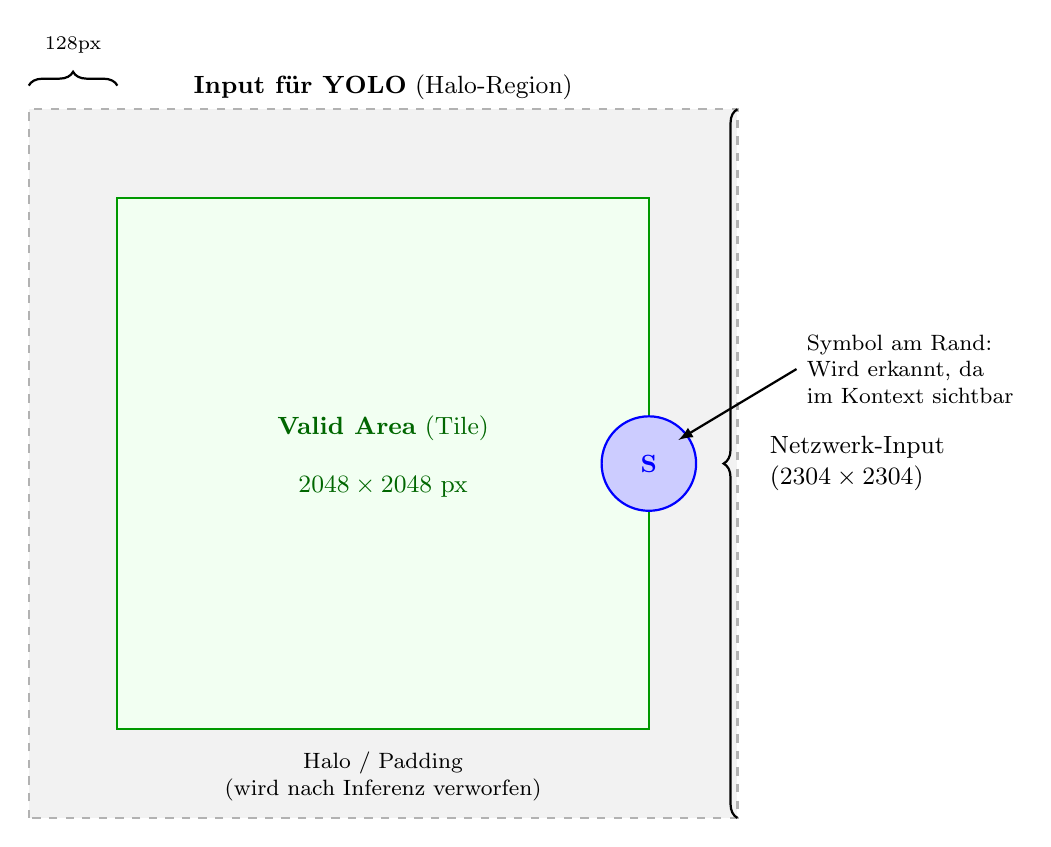
\begin{tikzpicture}[
        scale=1.5, 
        >=latex,
        font=\small
    ]
    
    % --- 1. Halo Region (Input für YOLO) ---
    % Graue Box außen
    \draw[fill=gray!10, dashed, thick, draw=gray!60] (0,0) rectangle (6,6);
    % Label oben
    \node[anchor=south] at (3,6) {\textbf{Input für YOLO} (Halo-Region)};
    
    % --- 2. Actual Tile (Valid Zone) ---
    % Grüne Box innen
    \draw[fill=green!5, thick, draw=green!60!black] (0.75,0.75) rectangle (5.25,5.25);
    \node[green!40!black] at (3,3.3) {\textbf{Valid Area} (Tile)};
    \node[green!40!black] at (3,2.8) {$2048 \times 2048$ px};
    
    % --- 3. Dimensionen (Braces/Klammern) ---
    % Wir nutzen braces für "wissenschaftlichen Look"
    \draw[decorate, decoration={brace, amplitude=5pt}, thick] (0, 6.2) -- (0.75, 6.2) 
        node[midway, above=8pt] {\scriptsize 128px};
        
    \draw[decorate, decoration={brace, amplitude=5pt}, thick] (6, 0) -- (6, 6) 
        node[midway, right=8pt, align=left] {Netzwerk-Input\\($2304 \times 2304$)};

    % --- 4. Symbol am Rand (Das Problem) ---
    % Ein Symbol, das auf der Kante liegt
    \draw[fill=blue!20, draw=blue, thick] (5.25, 3) circle (0.4);
    \node[blue] at (5.25, 3) {\textbf{S}};
    
    % Erklärungspfeil zum Symbol
    \draw[<-, thick] (5.5, 3.2) -- (6.5, 3.8) node[right, align=left, font=\footnotesize] {Symbol am Rand:\\Wird erkannt, da\\im Kontext sichtbar};

    % --- 5. Halo-Beschriftung ---
    \node[font=\footnotesize, align=center] at (3, 0.35) {Halo / Padding\\(wird nach Inferenz verworfen)};

    \end{tikzpicture}
    \caption{Visualisierung der Halo-Strategie}
    \label{fig:halo_tiling}
\end{figure}
\FloatBarrier
Der Halo-Bereich von 128 Pixeln dient als zusätzlicher Kontextbereich um jedes Tile und ist unabhängig vom Overlap. Während der Overlap (256 Pixel) die Mindestüberlappung zwischen benachbarten Tiles definiert, um Objekte an Tile-Grenzen zu erfassen, stellt der Halo sicher, dass Objekte nahe dem Tile-Rand ausreichend Kontextinformation für eine zuverlässige Erkennung haben. Detektionen, deren Zentrum im Halo-Bereich liegt, werden beim NMS-Schritt gefiltert.
\subsubsection{Winkeladaptive Parameterauswahl}
\label{subsubsec:winkelnormalisierung}
Eine Besonderheit der Implementierung besteht in der winkeladaptiven Anpassung der Bounding-Box-Parameter für jede Detektion. Nach der initialen YOLO-Detektion, die eine OBB in Form von $(c_x, c_y, w, h, \theta)$ liefert, werden die Dimensionen $w$ und $h$ sowie das Padding basierend auf dem Rotationswinkel $\theta$ angepasst.

Zunächst wird der Winkel normalisiert, um eine kanonische Repräsentation zu erhalten. Die Normalisierung erfolgt durch:

\begin{equation}
\theta_{\text{norm}} = \begin{cases}
\theta - \frac{\pi}{2}, & \text{falls } \theta > \frac{\pi}{4} \\
\theta + \frac{\pi}{2}, & \text{falls } \theta < -\frac{\pi}{4} \\
\theta, & \text{sonst}
\end{cases}
\end{equation}

Diese Normalisierung stellt sicher, dass der Winkel im Bereich $[-\frac{\pi}{4}, \frac{\pi}{4}]$ liegt. Falls eine Rotation außerhalb dieses Bereichs erforderlich ist, werden Breite und Höhe vertauscht:

\begin{equation}
(w_{\text{norm}}, h_{\text{norm}}) = \begin{cases}
(h, w), & \text{falls Rotation durchgeführt} \\
(w, h), & \text{sonst}
\end{cases}
\end{equation}

Basierend auf dem normalisierten Winkel $\theta_{\text{norm}}$ wird entschieden, ob das Symbol als horizontal, vertikal oder angular orientiert klassifiziert wird:

\begin{equation}
\text{Orientierung} = \begin{cases}
\text{Horizontal}, & \text{falls } |\theta_{\text{norm}}| < 15^\circ \text{ oder } |\theta_{\text{norm}} - 180^\circ| < 15^\circ \\
\text{Vertikal}, & \text{falls } |\theta_{\text{norm}} - 90^\circ| < 15^\circ \text{ oder } |\theta_{\text{norm}} - 270^\circ| < 15^\circ \\
\text{Angular}, & \text{sonst}
\end{cases}
\end{equation}

Für jede Orientierung werden unterschiedliche Expansionsfaktoren $(e_x, e_y)$ und Padding-Werte $p$ angewendet:

\begin{table}[H]
\centering
\begin{tabular}{|l|c|c|c|}
\hline
\textbf{Orientierung} & \textbf{$e_x$} & \textbf{$e_y$} & \textbf{$p$ [Pixel]} \\
\hline
Horizontal & 2.5 & 1.5 & 16 \\
Vertikal & 1.5 & 2.5 & 16 \\
Angular & 2.0 & 2.0 & 24 \\
\hline
\end{tabular}
\caption{Winkeladaptive Bounding-Box-Parameter}
\label{tab:angle_adaptive_params}
\end{table}

Die effektiven Dimensionen der Bounding Box werden dann berechnet als:

\begin{equation}
\begin{aligned}
w_{\text{eff}} &= w_{\text{norm}} \cdot e_x + 2p \\
h_{\text{eff}} &= h_{\text{norm}} \cdot e_y + 2p
\end{aligned}
\end{equation}

Diese Anpassung ist kritisch für die nachfolgende OCR, da bei horizontal orientierten Texten mehr horizontaler Kontext benötigt wird (z.B. für Texte wie \enquote{Signal A123}), während bei vertikal orientierten Texten mehr vertikaler Kontext erforderlich ist. Angular orientierte Objekte erhalten symmetrische Expansion und erhöhtes Padding, um Rotationseffekte auszugleichen.

\begin{figure}[H]
    \centering
    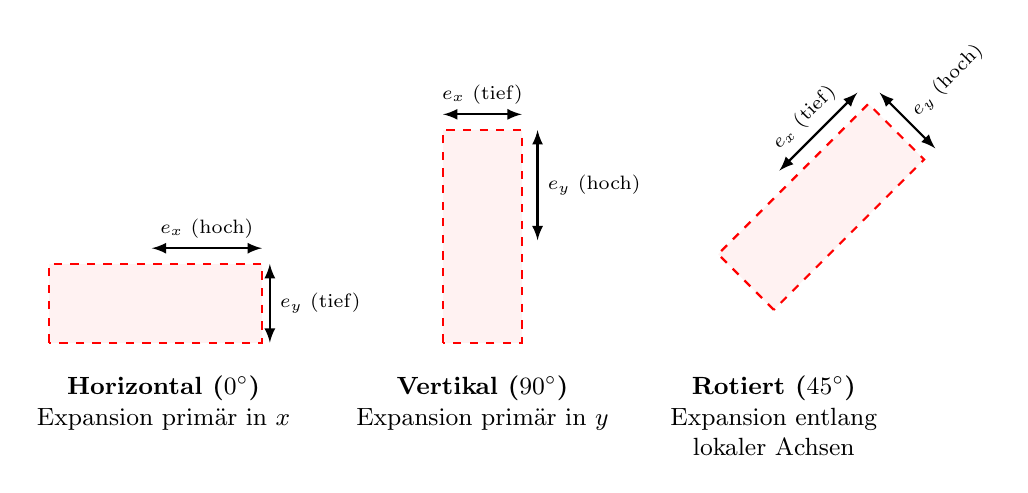
\begin{tikzpicture}[
        scale=1.0, 
        >=latex, 
        font=\small,
        symbol/.style={fill=blue!20, draw=blue!80!black, thick},
        roi/.style={draw=red, dashed, thick, fill=red!5},
        dim_arrow/.style={<->, thick, black}
    ]

    % --- 1. Horizontal (0°) ---
    \begin{scope}[local bounding box=scope1]
        \draw[symbol] (0,0) rectangle (1, 0.6);
        \node[blue!80!black] at (0.5, 0.3) {\textbf{S}};
        \node[black, anchor=west] at (1.2, 0.3) {Text};
        
        \draw[roi] (-0.2, -0.2) rectangle (2.5, 0.8);
        
        % Dimensions
        \draw[dim_arrow] (1.1, 1.0) -- (2.5, 1.0) node[midway, above, font=\scriptsize] {$e_x$ (hoch)};
        \draw[dim_arrow] (2.6, -0.2) -- (2.6, 0.8) node[midway, right, font=\scriptsize] {$e_y$ (tief)};
        
        \node[align=center, anchor=north] at (1.25, -0.5) {\textbf{Horizontal ($0^\circ$)}\\Expansion primär in $x$};
    \end{scope}

    % --- 2. Vertikal (90°) ---
    \begin{scope}[shift={(5,0)}, local bounding box=scope2]
        \draw[symbol] (0,0) rectangle (0.6, 1);
        \node[blue!80!black] at (0.3, 0.5) {\rotatebox{90}{\textbf{S}}};
        \node[black, anchor=south] at (0.3, 1.2) {\rotatebox{90}{Text}};
        
        \draw[roi] (-0.2, -0.2) rectangle (0.8, 2.5);
        
        % Dimensions
        \draw[dim_arrow] (1.0, 1.1) -- (1.0, 2.5) node[midway, right, font=\scriptsize] {$e_y$ (hoch)};
        \draw[dim_arrow] (-0.2, 2.7) -- (0.8, 2.7) node[midway, above, font=\scriptsize] {$e_x$ (tief)};

        \node[align=center, anchor=north] at (0.3, -0.5) {\textbf{Vertikal ($90^\circ$)}\\Expansion primär in $y$};
    \end{scope}

    % --- 3. Angular (45°) ---
    \begin{scope}[shift={(9,0.5)}, local bounding box=scope3]
        % Rotation Scope
        \begin{scope}[rotate=45]
            % Symbol & Text
            \draw[symbol] (0,0) rectangle (1, 0.6);
            \node[blue!80!black, rotate=45] at (0.5, 0.3) {\textbf{S}};
            \node[black, rotate=45, anchor=west] at (1.2, 0.3) {Text};
            
            % ROI
            \draw[roi] (-0.2, -0.2) rectangle (2.5, 0.8);

            % --- NEW: MISSING ARROWS ADDED HERE ---
            % Dimension e_x (parallel to top edge)
            \draw[dim_arrow] (1.1, 1.0) -- (2.5, 1.0) 
                node[midway, above, font=\scriptsize, rotate=45] {$e_x$ (tief)};
            
            % Dimension e_y (parallel to right edge)
            \draw[dim_arrow] (2.7, -0.2) -- (2.7, 0.8) 
                node[midway, right, font=\scriptsize, rotate=45] {$e_y$ (hoch)};
        \end{scope}
        
        \node[align=center, anchor=north] at (0, -1.0) {\textbf{Rotiert ($45^\circ$)}\\Expansion entlang\\lokaler Achsen};
    \end{scope}

    \end{tikzpicture}
    \caption{Adaptive Expansion der Region of Interest (ROI)}
    \label{fig:adaptive_padding}
\end{figure}
Abbildung \ref{fig:adaptive_padding} visualisiert diese Anpassung für die drei Orientierungskategorien. Im Fall angular orientierter Objekte (rechts) erfolgt die Expansion entlang der rotierten Objektachsen.
\subsubsection{Post-Processing und Duplikatentfernung}

Nach der Inferenz auf allen Tiles müssen die Detektionen aggregiert und Duplikate entfernt werden. Die Koordinaten-Rücktransformation erfolgt durch Addition der Tile-Offsets:

\begin{equation}
\begin{aligned}
c_x^{\text{global}} &= c_x^{\text{lokal}} + x_{\text{Tile}} \\
c_y^{\text{global}} &= c_y^{\text{lokal}} + y_{\text{Tile}}
\end{aligned}
\end{equation}

Aufgrund der Überlappung zwischen Tiles werden Objekte im Überlappungsbereich mehrfach detektiert. Zur Eliminierung dieser Duplikate wird eine Non-Maximum Suppression (NMS) durchgeführt. Die NMS arbeitet klassenweise und behält für jede Klasse nur die Detektionen mit höchster Konfidenz bei, wenn mehrere Detektionen dasselbe Objekt beschreiben.

Der Überlappungsgrad zweier Bounding Boxes wird mittels Intersection over Union (IoU) quantifiziert:

\begin{equation}
\text{IoU}(B_1, B_2) = \frac{\text{Area}(B_1 \cap B_2)}{\text{Area}(B_1 \cup B_2)}
\end{equation}

Der NMS-Algorithmus funktioniert wie folgt:

\begin{enumerate}
    \item Sortiere alle Detektionen einer Klasse nach absteigender Konfidenz
    \item Wähle die Detektion mit höchster Konfidenz und füge sie zur Ergebnismenge hinzu
    \item Entferne alle Detektionen, deren IoU mit der gewählten Detektion einen klassenspezifischen Schwellenwert $\tau_{\text{NMS}}$ überschreitet
    \item Wiederhole Schritte 2-3, bis keine Detektionen mehr vorhanden sind
\end{enumerate}

Die NMS-Schwellenwerte sind klassenspezifisch konfiguriert:

\begin{table}[H]
\centering
\begin{tabular}{|l|r|p{7cm}|}
\hline
\textbf{Klasse} & \textbf{$\tau_{\text{NMS}}$} & \textbf{Begründung} \\
\hline
coordinate & 0.3 & Strenger Schwellenwert, da Koordinaten oft dicht gruppiert sind \\
signal & 0.5 & Standard-Schwellenwert für mittlere Objektdichte \\
weichen\_block & 0.6 & Lockerer Schwellenwert für große Symbole mit natürlicher Varianz \\
default & 0.5 & Fallback für nicht explizit konfigurierte Klassen \\
\hline
\end{tabular}
\caption{Klassenspezifische NMS-Schwellenwerte}
\label{tab:nms_thresholds}
\end{table}

Zusätzlich zur NMS werden Detektionen unterhalb klassenspezifischer Konfidenzschwellen verworfen. Diese Schwellen wurden empirisch auf dem Validierungssatz optimiert, um ein Gleichgewicht zwischen Precision und Recall zu erreichen.

\subsubsection{Ausgabeformat}

Das Ergebnis der Objekterkennungsstufe ist eine strukturierte Liste aller detektierten Symbole, wobei jede Detektion durch folgende Attribute charakterisiert ist:

\begin{itemize}
    \item \textbf{Klassenname} und \textbf{Klassenindex}: Semantische Kategorie des Symbols
    \item \textbf{Konfidenz}: Wahrscheinlichkeit der Korrektheit der Detektion im Intervall $[0, 1]$
    \item \textbf{AABB-Koordinaten} $(x_1, y_1, x_2, y_2)$: Achsenparallele Bounding Box für UI-Darstellung
    \item \textbf{OBB-Parameter} $(c_x, c_y, w_{\text{eff}}, h_{\text{eff}}, \theta_{\text{norm}})$: Rotierte Bounding Box für OCR
    \item \textbf{Polygon-Eckpunkte} $\{(x_i, y_i)\}_{i=1}^{4}$: Exakte Umrisspolygone
    \item \textbf{Seitennummer}: Zuordnung zur entsprechenden PDF-Seite
\end{itemize}

Diese strukturierte Repräsentation dient als Eingabe für die nachfolgende OCR-Stufe, welche die Textinformationen in unmittelbarer Nähe der detektierten Symbole extrahiert.

\subsubsection{Performance-Charakteristika}

Die durchschnittliche Inferenzzeit pro Tile beträgt ca. 120 ms auf einer Standard-CPU (Intel Core i7 der 10. Generation). Für einen typischen A3-Gleisplan mit ca. 12-16 Tiles ergibt sich eine Gesamtverarbeitungszeit von ca. 15-20 Sekunden für die Objekterkennungsstufe. Diese CPU-basierte Inferenz wurde bewusst gewählt, um die Einsetzbarkeit der Software auf Standard-Workstations ohne dedizierte GPU zu gewährleisten, was die Verbreitung und Nutzung im Produktivumfeld erleichtert.

\section{Orientierungsadaptive OCR-Pipeline}
\label{sec:ocrpipeline}
Die Texterkennung aus den detektierten Symbolen stellt eine zentrale Herausforderung dar, 
da die Textregionen beliebig im Gleisplan rotiert sein können. Dieses Kapitel beschreibt 
die implementierte OCR-Pipeline, die durch Multi-Engine-Kaskadierung, rotationsadaptive 
Strategien und klassenspezifische Bildvorverarbeitung eine robuste Texterkennung ermöglicht 
und damit die Anforderungen \textbf{FA-004} (OCR-Genauigkeit) und \textbf{FA-005} 
(OCR-Robustheit) adressiert.

\subsection{Multi-Engine Kaskadierung}

Das System implementiert eine kaskadierende Architektur mit drei OCR-Engines: PaddleOCR als primäre Engine, Tesseract als Fallback-Engine und optional EasyOCR für schwierige Fälle. Die Grundidee dieser Kaskadierung ist, dass verschiedene OCR-Engines unterschiedliche Stärken haben. PaddleOCR ist schnell und präzise bei gut ausgerichteten Texten, Tesseract ist besonders robust bei verrauschten oder pixeligen Bildern, und EasyOCR ist spezialisiert auf schwierige Winkel und perspektivische Verzerrungen.

\subsubsection{Funktionsweise der Kaskadierung}

Die Kaskadierung funktioniert nach einem sequenziellen Prinzip. Zunächst wird PaddleOCR auf dem Bildausschnitt ausgeführt, und zwar viermal mit unterschiedlichen Rotationswinkeln: $0^\circ, 90^\circ, 180^\circ und 270^\circ$. Der Grund für diese vier Rotationen ist, dass PaddleOCR am besten mit horizontal ausgerichtetem Text funktioniert. Durch das Ausprobieren aller vier Hauptrichtungen wird sichergestellt, dass mindestens eine Rotation den Text horizontal ausrichtet.

Für jede dieser Rotationen wird das OCR-Ergebnis durch eine klassenspezifische Validierungsfunktion geprüft. Diese Validierung überprüft, ob der erkannte Text dem erwarteten Muster der jeweiligen Symbolklasse entspricht. Beispielsweise muss ein Signal-Text mit einem Großbuchstaben beginnen, gefolgt von 1-3 Ziffern (wie \enquote{A12} oder \enquote{B234}). Zusätzlich zur Mustererkennung wird der Konfidenz-Wert (Vertrauenswert) des OCR-Ergebnisses überprüft.

Der Konfidenz-Wert von PaddleOCR liegt typischerweise zwischen 0 und etwa 2, wobei höhere Werte eine größere Sicherheit bedeuten. Ein empirisch bestimmter Schwellenwert von 1.3 hat sich als optimal erwiesen: Ergebnisse über diesem Wert sind in der Regel korrekt, während niedrigere Werte oft Fehler enthalten. Dieser Schwellenwert wurde durch Tests auf dem Trainingsdatensatz bestimmt und stellt einen guten Kompromiss zwischen Präzision (wie viele der als \enquote{korrekt} markierten Ergebnisse wirklich korrekt sind) und Recall (wie viele der tatsächlich vorhandenen Texte erkannt werden) dar.

Wenn PaddleOCR bei keiner der vier Rotationen ein validiertes Ergebnis mit ausreichender Konfidenz liefert, wird Tesseract als Fallback-Engine aktiviert. Tesseract verwendet einen anderen Algorithmus als PaddleOCR und ist besonders robust gegenüber verrauschten oder pixeligen Bildern. Tesseract wird mit dem Page Segmentation Mode 7 konfiguriert, der das Bild als einzelne Textzeile behandelt-eine Annahme, die für die kurzen Symbol-Beschriftungen im Gleisplan zutreffend ist.

Falls auch Tesseract kein valides Ergebnis liefert und die optionale dritte Engine EasyOCR aktiviert ist, wird diese als letzte Instanz aufgerufen. EasyOCR ist besonders gut bei stark geneigten oder perspektivisch verzerrten Texten, benötigt aber erheblich mehr Rechenzeit (etwa 5-10 Mal langsamer als PaddleOCR).

\subsubsection{Konfiguration der OCR-Engines}

Jede OCR-Engine wurde mit spezifischen Parametern konfiguriert, um optimale Ergebnisse für die Domäne der Gleispläne zu erzielen.

\textbf{PaddleOCR} wurde mit den folgenden Einstellungen verwendet:
\begin{itemize}
    \item \textbf{Detection Model}: \enquote{ch\_PP-OCRv4\_det} - ein vortrainiertes Modell zur Textlokalisierung, das ursprünglich für chinesische Dokumente entwickelt wurde, aber auch für deutsche/englische Texte ausgezeichnet funktioniert
    \item \textbf{Recognition Model}: \enquote{ch\_PP-OCRv4\_rec} - das zugehörige Erkennungsmodell für die eigentliche Zeichenerkennung
    \item \textbf{Angle Classification}: Aktiviert - ermöglicht automatische Erkennung und Korrektur der Textorientierung
    \item \textbf{Sprache}: \enquote{en} (Englisch) - da die meisten Beschriftungen alphanumerisch sind
\end{itemize}

\textbf{Tesseract} wurde mit den folgenden Parametern konfiguriert:
\begin{itemize}
    \item \textbf{Page Segmentation Mode (psm)}: 7 - behandelt das Bild als einzelne Textzeile, was für kurze Symbol-Beschriftungen optimal ist
    \item \textbf{OCR Engine Mode (oem)}: 3 - verwendet den LSTM-basierten neuronalen Netzwerk-Modus, der die beste Genauigkeit bietet
    \item \textbf{Character Whitelist}: Beschränkt auf \enquote{0123456789ABCDEFGHIJKLMNOPQRSTUVWXYZ+-.} - dies verhindert, dass Tesseract falsche Sonderzeichen oder Kleinbuchstaben erkennt, die in den meisten Symbolklassen nicht vorkommen
\end{itemize}

Die Whitelist ist besonders wichtig, da sie die Fehlerrate deutlich reduziert. Ohne diese Einschränkung würde Tesseract manchmal exotische Sonderzeichen oder Umlaute erkennen, die in technischen Gleisplänen nie vorkommen.

\textbf{EasyOCR} wurde mit minimaler Konfiguration verwendet:
\begin{itemize}
    \item \textbf{Sprachen}: [\enquote{en}] - Englisch als Basissprache
    \item \textbf{GPU-Nutzung}: Aktiviert - beschleunigt die Verarbeitung erheblich, wenn eine GPU verfügbar ist
\end{itemize}



\begin{figure}[H]
\centering
\begin{tikzpicture}[
    % Moderne Bibliothek für Positionierung
    scale=0.75,
    transform shape,
    node distance=1.0cm and 1.5cm, % Vertikaler und Horizontaler Abstand
    % Styles
    box/.style={
        rectangle, 
        draw=blue!60!black, 
        fill=blue!5, 
        text width=3cm, 
        align=center, 
        rounded corners, 
        minimum height=1cm,
        thick
    },
    decision/.style={
        diamond, 
        draw=orange!60!black, 
        fill=orange!10, 
        text width=2cm, 
        align=center, 
        aspect=2, 
        thick,
        inner sep=0pt
    },
    arrow/.style={
        ->, 
        >=latex, % Schönere Pfeilspitze
        thick, 
        rounded corners=5pt % Abgerundete Ecken für professionellen Look
    }
]

% --- NODES (mit positioning library) ---
\node[box] (start) {Bildausschnitt extrahieren};

\node[box, below=of start] (paddle) {PaddleOCR\\(4 Rotationen)};

\node[decision, below=of paddle] (check1) {Konfidenz\\$> 1.3$?};

% "right=of" statt "right of=" verhindert Überlappung
\node[box, right=of check1, xshift=0.5cm] (accept1) {Ergebnis\\akzeptieren};

\node[box, below=of check1] (tesseract) {Tesseract\\OCR};

\node[decision, below=of tesseract] (check2) {Regex\\validiert?};

\node[box, right=of check2, xshift=0.5cm] (accept2) {Ergebnis\\akzeptieren};

\node[box, below=of check2] (easyocr) {EasyOCR\\(optional)};

\node[box, below=of easyocr] (final) {Finales\\Ergebnis};


% --- ARROWS ---
% Standard Pfade (Links)
\draw[arrow] (start) -- (paddle);
\draw[arrow] (paddle) -- (check1);

% Check 1 Pfade
\draw[arrow] (check1) -- node[above, font=\footnotesize] {Ja} (accept1);
\draw[arrow] (check1) -- node[right, font=\footnotesize] {Nein} (tesseract);

% Tesseract -> Check 2
\draw[arrow] (tesseract) -- (check2);

% Check 2 Pfade
\draw[arrow] (check2) -- node[above, font=\footnotesize] {Ja} (accept2);
\draw[arrow] (check2) -- node[right, font=\footnotesize] {Nein} (easyocr);

% EasyOCR -> Final
\draw[arrow] (easyocr) -- (final);


% --- HIER IST DER TRICK FÜR DIE RECHTEN LINIEN ---

% Linie von Accept 1 (Ganz außen)
% ++(2.0, 0) heißt: Gehe vom Knoten 2cm nach rechts, bevor du abbiegst
\draw[arrow] (accept1.east) -- ++(1.5, 0) |- (final.east);

% Linie von Accept 2 (Etwas weiter innen)
% ++(0.7, 0) heißt: Gehe vom Knoten 0.7cm nach rechts (weniger als oben)
% |- ([yshift=2mm]final.east) versetzt den Pfeil am Ende etwas nach oben, damit sie sich nicht treffen
\draw[arrow] (accept2.east) -- ++(0.5, 0) |- ([yshift=2mm]final.east);

\end{tikzpicture}
\caption{Ablaufdiagramm der Multi-Engine OCR-Kaskadierung}
\label{fig:ocr_cascade}
\end{figure}
\FloatBarrier

\subsection{Dual-Winkel-Routing System}
\label{subsec:dualwinkelrouting}
Eine zentrale Herausforderung bei der OCR ist die beliebige Rotation der Symbole im Gleisplan. Während einige Symbole horizontal ausgerichtet sind, können andere um $ 45^\circ, 30^\circ$ oder sogar beliebige Winkel gedreht sein. Um diese Vielfalt zu bewältigen, wurde ein Dual-Path-Routing-System implementiert, das zwischen zwei verschiedenen Verarbeitungswegen unterscheidet.

\subsubsection{Cardinal Path und Angular Path}

Das System unterscheidet zwischen dem \textbf{Cardinal Path} (für nahezu horizontal/vertikal ausgerichtete Texte) und dem \textbf{Angular Path} (für beliebig gedrehte Texte). Die Entscheidung, welcher Pfad verwendet wird, basiert auf dem Rotationswinkel der Bounding Box.

Zunächst wird der von YOLO gelieferte Winkel normalisiert. Da YOLO Winkel im Bereich von $0^\circ$ bis $360^\circ$ liefern kann, werden Winkel über $180^\circ$ durch Subtraktion von $360^\circ$ in den Bereich $-180^\circ$ bis $180^\circ$ transformiert. Ein Winkel von $270^\circ$ wird beispielsweise zu $-90^\circ$. Dies vereinfacht die Logik erheblich, da nun positive Winkel eine Drehung gegen den Uhrzeigersinn und negative Winkel eine Drehung im Uhrzeigersinn darstellen.

Anschließend wird geprüft, ob der Absolutwert des normalisierten Winkels unter $15^\circ$ liegt. Diese $15^\circ$ wurden empirisch durch Experimente bestimmt: Bei Winkeln bis zu dieser Größe liefert eine einfache Rotation auf den nächsten kardinalen Winkel ($0^\circ, 90^\circ, 180^\circ$ oder $270^\circ$) bessere Ergebnisse als eine komplexe Perspektiventransformation. Der Grund ist, dass bei kleinen Winkeln die Perspektiventransformation zu leichten Verzerrungen führen kann, während die diskrete Rotation verlustfrei ist.

\textbf{Cardinal Path (Winkel $\leq$ $15^\circ$):} Wenn der Winkel nahe an einem kardinalen Wert liegt, wird der Bildausschnitt einfach auf den nächstgelegenen kardinalen Winkel rotiert. Die Rotation erfolgt mittels einer Standard-Rotationsmatrix, die das Bild um den Mittelpunkt dreht. Diese Methode ist schnell, einfach und vermeidet Interpolationsartefakte, da nur $90^\circ$ Schritte verwendet werden.

Konkret wird aus den vier Kandidaten ($0^\circ, 90^\circ, 180^\circ, 270^\circ$) derjenige gewählt, der die kleinste Winkeldifferenz zum normalisierten Winkel hat. Ein Winkel von $12^\circ$ wird also auf $0^\circ$ rotiert, ein Winkel von $85^\circ$ auf $90^\circ$, und so weiter.


\textbf{Angular Path (Winkel > $15^\circ$):} Bei größeren Abweichungen von den kardinalen Winkeln wird eine Perspektiventransformation verwendet. Diese Methode nutzt die vier Eckpunkte der Oriented Bounding Box (OBB), um eine Transformationsmatrix zu berechnen. Die Transformation wandelt die gedrehte OBB in ein achsenparalleles Rechteck um, wodurch der Text horizontal ausgerichtet wird.

Die Perspektiventransformation wird mit OpenCV's \texttt{getPerspectiveTransform()}-Funktion implementiert. Diese Funktion benötigt zwei Sätze von je vier Punkten: die Quellpunkte (die vier Ecken der gedrehten OBB) und die Zielpunkte (die vier Ecken eines aufrechten Rechtecks). Aus diesen acht Punkten berechnet die Funktion eine 3x3-Transformationsmatrix, die dann mit \texttt{warpPerspective()} auf das Bild angewendet wird.

Obwohl diese Methode rechenintensiver ist (etwa 2-3 Mal langsamer als eine einfache Rotation), liefert sie bei beliebigen Winkeln deutlich bessere Ergebnisse, da der Text exakt horizontal ausgerichtet wird, nicht nur annähernd.

\begin{figure}[H]
\centering
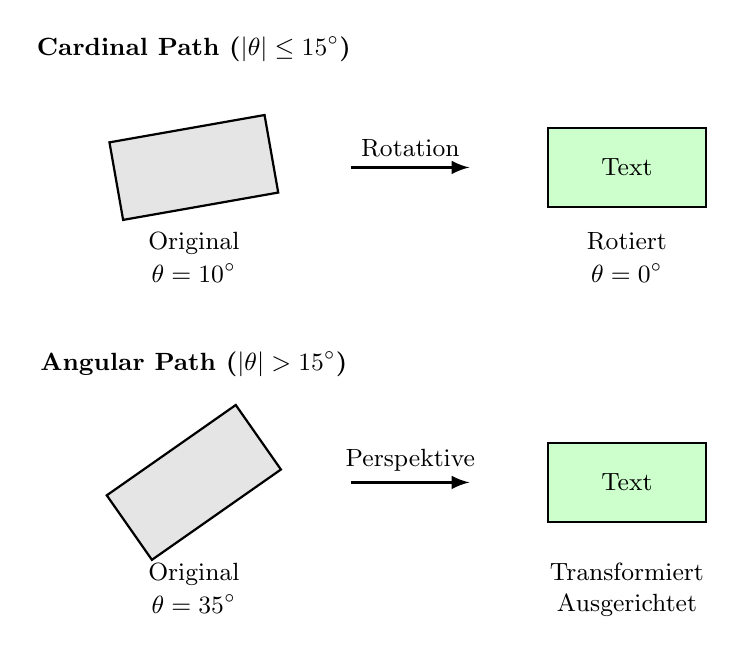
\begin{tikzpicture}[
    >=latex, 
    font=\small,
    % Styles für Konsistenz
    box/.style={thick, fill=gray!20},
    result/.style={thick, fill=green!20},
    arrow/.style={->, very thick}
]

% --- OBERER TEIL: CARDINAL PATH ---
\begin{scope}[yshift=0cm] % Lokaler Bereich oben
    \node at (0, 1.5) {\textbf{Cardinal Path ($|\theta| \leq 15^\circ$)}};

    % Original (lokal rotiert um 0,0)
    \draw[box, rotate=10] (-1, -0.5) rectangle (1, 0.5);
    \node[below=0.7cm] at (0,0) {Original};
    \node[below=1.1cm] at (0,0) {$\theta = 10^\circ$};

    % Pfeil
    \draw[arrow] (2, 0) -- (3.5, 0) node[midway, above] {Rotation};

    % Ergebnis
    \draw[result] (4.5, -0.5) rectangle (6.5, 0.5);
    \node at (5.5, 0) {Text};
    \node[below=0.7cm] at (5.5,0) {Rotiert};
    \node[below=1.1cm] at (5.5,0) {$\theta = 0^\circ$};
\end{scope}


% --- UNTERER TEIL: ANGULAR PATH ---
% Wir verschieben den ganzen Block nach unten (y = -4cm)
\begin{scope}[yshift=-4cm] 
    \node at (0, 1.5) {\textbf{Angular Path ($|\theta| > 15^\circ$)}};

    % Original (Jetzt zentriert gezeichnet, Rotation wirkt lokal!)
    \draw[box, rotate=35] (-1, -0.5) rectangle (1, 0.5);
    
    % Labels sitzen nun perfekt unter dem Kasten
    \node[below=0.9cm] at (0,0) {Original};
    \node[below=1.3cm] at (0,0) {$\theta = 35^\circ$};

    % Pfeil
    \draw[arrow] (2, 0) -- (3.5, 0) node[midway, above] {Perspektive};

    % Ergebnis
    \draw[result] (4.5, -0.5) rectangle (6.5, 0.5);
    \node at (5.5, 0) {Text};
    \node[below=0.9cm] at (5.5,0) {Transformiert};
    \node[below=1.3cm] at (5.5,0) {Ausgerichtet};
\end{scope}

\end{tikzpicture}
\caption{Vergleich: Cardinal Path vs. Angular Path Rotationsstrategien}
\label{fig:dual_path}
\end{figure}
Abbildung~\ref{fig:angular_ocr_example} demonstriert die erfolgreiche Verarbeitung eines um $37,5^\circ$ rotierten Koordinatentexts durch den Angular Path.



Das System erkannte den Koordinatentext \texttt{0.0629} korrekt trotz der nicht-kardinalen Orientierung von $\theta = -37{,}5^\circ$. Die Perspektiventransformation richtete die gedrehte Oriented Bounding Box horizontal aus, wodurch PaddleOCR mit einer Konfidenz von 0.95 den Text extrahieren konnte. Die erfolgreiche Verknüpfung mit dem benachbarten Symbol (Gl.112) validiert sowohl die OCR-Robustheit (FA-005) als auch die Rotationsinvarianz (FA-002) für beliebige Winkel außerhalb der kardinalen Orientierungen.

\begin{figure}[H]
\centering
\includegraphics[width=0.65\textwidth]{images/Kapitel6/angulartextv1.png}
\caption{Verarbeitung eines um $37,5^\circ$ rotierten Elemente durch Angular-Path-OCR}
\label{fig:angular_ocr_example}
\end{figure}
\subsection{Klassenspezifische Strategien}

Verschiedene Symbolklassen im Gleisplan haben unterschiedliche visuelle Eigenschaften, die spezielle Vorverarbeitungsschritte erfordern. Signale haben beispielsweise oft einen farbigen Hintergrund und größere Beschriftungen, während GKS häufig von dünnen Linien umgeben sind und sehr kompakte Texte haben. Um diese Unterschiede zu berücksichtigen, wurde für jede Klasse eine spezialisierte Verarbeitungsstrategie implementiert.

\subsubsection{Adaptive Padding}

Das Padding erweitert den von YOLO gelieferten Bildausschnitt, um sicherzustellen, dass der gesamte Text erfasst wird. Oft liegt der Text teilweise außerhalb der detektierten Bounding Box, besonders bei Signalen, wo die Beschriftung über oder neben dem eigentlichen Symbol sein kann.

Die Größe des Paddings wird primär relativ zur Größe der Bounding Box berechnet. Um jedoch auch bei sehr schmalen Objekten (z.B. Signalmasten) eine Mindesterfassung zu gewährleisten, wird zusätzlich ein absolutes Minimum pmin=10 Pixel definiert. Die Berechnung erfolgt durch:

\begin{equation} 
    p_x = \max(\alpha \cdot w_{\text{bbox}}, p_{\text{min}}), \quad p_y = \max(\beta \cdot h_{\text{bbox}}, p_{\text{min}}) 
\end{equation}

wobei $p_x$ das horizontale Padding (in Pixeln), $p_y$ das vertikale Padding (in Pixeln), $w_{\text{bbox}}$ die Breite der Bounding Box, $h_{\text{bbox}}$ die Höhe der Bounding Box, und $\alpha$ sowie $\beta$ klassenspezifische Faktoren sind.

Die folgende Tabelle zeigt die optimierten Faktoren für jede Symbolklasse:

\begin{table}[H]
\centering
\begin{tabular}{|l|c|c|p{5cm}|}
\hline
\textbf{Klasse} & $\boldsymbol{\alpha}$ & $\boldsymbol{\beta}$ & \textbf{Begründung} \\
\hline
Signal & 0.2 & 0.3 & Beschriftung oft oberhalb des Symbols \\
GKS (beide Typen) & 0.15 & 0.15 & Kompakte, zentrierte Beschriftung \\
Weiche & 0.1 & 0.1 & Text direkt am Symbol \\
Koordinate & 0.25 & 0.25 & Längere Zahlenfolgen, mehr Platz nötig \\
\hline
\end{tabular}
\caption{Klassenspezifische Padding-Faktoren und deren Begründung}
\end{table}

Für Signale wurde beispielsweise ein Faktor von $\alpha = 0.2$ (20\% der Breite) und $\beta = 0.3$ (30\% der Höhe) als optimal ermittelt. Das größere vertikale Padding berücksichtigt, dass Signal-Beschriftungen typischerweise oberhalb des Symbols positioniert sind. Bei einer Bounding Box von $100 \times 50$ Pixeln würde dies ein Padding von 20 Pixeln horizontal und 15 Pixeln vertikal bedeuten.

Das finale erweiterte Bild hat dann die Dimensionen $(h + 2p_y) \times (w + 2p_x)$, wobei das \enquote{2} berücksichtigt, dass das Padding sowohl oben und unten als auch links und rechts hinzugefügt wird.

\subsubsection{Morphologische Filterung für GKS}

GKS-Symbole sind häufig von dünnen Linien umgeben, die die OCR-Qualität beeinträchtigen können. Diese Linien können fälschlicherweise als Buchstaben wie \enquote{I}, \enquote{l} oder \enquote{1} interpretiert werden. Um diese Störungen zu reduzieren, wird ein morphologischer Opening-Filter angewendet.

Opening ist eine Kombination aus zwei aufeinanderfolgenden Operationen: Zunächst wird eine \textbf{Erosion} durchgeführt, die kleine helle Strukturen (wie dünne Linien) entfernt. Anschließend wird eine \textbf{Dilation} durchgeführt, die die verbleibenden Strukturen (die Textzeichen) wieder auf ihre ursprüngliche Größe erweitert. Der Effekt ist, dass dünne Linien komplett verschwinden, während dickere Strukturen (Buchstaben und Zahlen) erhalten bleiben.

Der Filter verwendet ein quadratisches strukturierendes Element mit der Größe 3x3 Pixel - also eine Matrix aus 9 Einsen. Diese Größe wurde gewählt, weil sie ausreicht, um typische Störlinien (1-2 Pixel dick) zu entfernen, aber nicht so groß ist, dass sie die Textzeichen selbst beschädigt. Die Anwendung erfolgt auf dem binärisierten Bild, wobei die Pixel entweder komplett weiß (Text) oder komplett schwarz (Hintergrund) sind.
\begin{figure}[H]
\centering
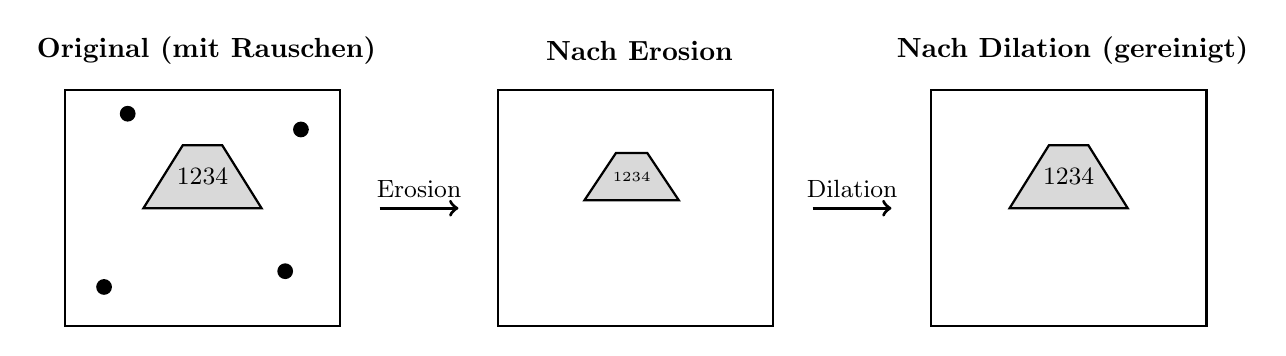
\begin{tikzpicture}

% Original with noise
\node at (1.8, 3.5) {\textbf{Original (mit Rauschen)}};
\draw[thick] (0, 0) rectangle (3.5, 3);
% GKS (trapezoid)
\draw[thick, fill=gray!30] (1, 1.5) -- (1.5, 2.3) -- (2, 2.3) -- (2.5, 1.5) -- cycle;
\node at (1.75, 1.9) {\small 1234};
% Noise pixels
\fill[black] (0.5, 0.5) circle (0.1cm);
\fill[black] (3, 2.5) circle (0.1cm);
\fill[black] (0.8, 2.7) circle (0.1cm);
\fill[black] (2.8, 0.7) circle (0.1cm);

% Arrow
\draw[->, very thick] (4, 1.5) -- (5, 1.5) node[midway, above] {\small Erosion};

% After erosion
\node at (7.3, 3.5) {\textbf{Nach Erosion}};
\draw[thick] (5.5, 0) rectangle (9, 3);
% Smaller GKS symbol
\draw[thick, fill=gray!30] (6.6, 1.6) -- (7, 2.2) -- (7.4, 2.2) -- (7.8, 1.6) -- cycle;
\node[font=\tiny] at (7.2, 1.9) {1234};

% Arrow
\draw[->, very thick] (9.5, 1.5) -- (10.5, 1.5) node[midway, above] {\small Dilation};

% After dilation (cleaned)
\node at (12.8, 3.5) {\textbf{Nach Dilation (gereinigt)}};
\draw[thick] (11, 0) rectangle (14.5, 3);
% Restored GKS symbol
\draw[thick, fill=gray!30] (12, 1.5) -- (12.5, 2.3) -- (13, 2.3) -- (13.5, 1.5) -- cycle;
\node at (12.75, 1.9) {\small 1234};

\end{tikzpicture}
\caption{Morphologisches Opening zur Rauschentfernung bei GKS-Symbolen}
\label{fig:morphology}
\end{figure}

\subsubsection{Multi-Scale Processing für Koordinaten}

Koordinaten-Beschriftungen sind oft klein und können bei niedriger Bildauflösung schwer lesbar sein. Ein typisches Problem: Bei einem eingescannten Gleisplan mit 150 DPI kann eine Koordinaten-Beschriftung nur 15-20 Pixel hoch sein, was für OCR-Engines an der Grenze der Lesbarkeit liegt.

Um dies zu kompensieren, wird ein Multi-Scale-Ansatz verwendet: Das Bild wird mit drei verschiedenen Skalierungsfaktoren vergrößert - 1.5x (50\% größer), 2.0x (doppelte Größe) und 2.5x (2.5-fache Größe). Die OCR wird auf allen drei Skalen durchgeführt, und am Ende wird das Ergebnis mit der höchsten Konfidenz ausgewählt.

Die Skalierung erfolgt mit Lanczos-Interpolation, einem hochwertigen Algorithmus, der scharfe Kanten erhält und keine Treppeneffekte oder Blockbildung verursacht. Lanczos ist zwar rechenintensiver als einfachere Methoden (wie bilineare Interpolation), liefert aber deutlich schärfere Ergebnisse, was bei der Vergrößerung kleiner Texte entscheidend ist.

Dieser Ansatz erhöht zwar die Rechenzeit erheblich (die OCR wird dreimal durchgeführt), verbessert aber die Erkennungsrate bei kleinen Texten von etwa 60\% auf über 85\%. Der Trade-off zwischen Geschwindigkeit und Genauigkeit wurde hier bewusst zugunsten der Genauigkeit entschieden, da Koordinaten kritische Informationen enthalten.

\subsection{Bildvorverarbeitungs-Algorithmen}

Vor der eigentlichen OCR-Verarbeitung werden die Bildausschnitte durch eine Reihe von Vorverarbeitungsschritten optimiert, um die Textqualität zu verbessern und störende Elemente zu entfernen.

\begin{figure}[H]
\centering
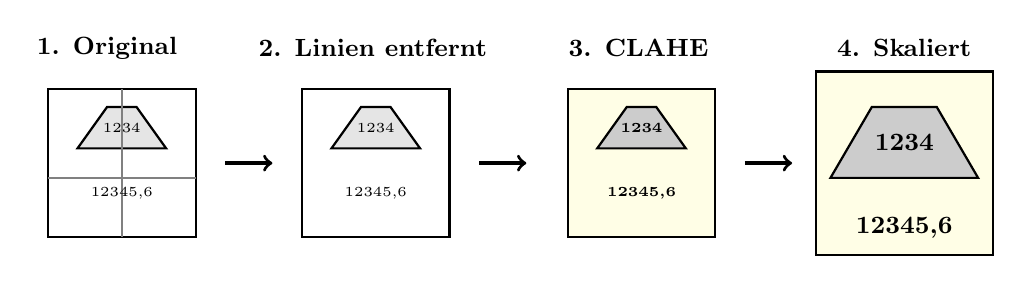
\begin{tikzpicture}[scale=0.75]

% Step 1: Original with lines
\node at (1, 3.2) {\small \textbf{1. Original}};
\draw[thick] (0, 0) rectangle (2.5, 2.5);
% GKS symbol (trapezoid)
\draw[thick, fill=gray!20] (0.5, 1.5) -- (1, 2.2) -- (1.5, 2.2) -- (2, 1.5) -- cycle;
\node at (1.25, 1.85) {\tiny 1234};
% Track lines (störende Gleislinien)
\draw[gray, thick] (0, 1) -- (2.5, 1);
\draw[gray, thick] (1.25, 0) -- (1.25, 2.5);
\node[below, font=\tiny] at (1.25, 1) {12345,6};

% Arrow
\draw[->, very thick] (3, 1.25) -- (3.8, 1.25);

% Step 2: Lines removed
\node at (5.5, 3.2) {\small \textbf{2. Linien entfernt}};
\draw[thick] (4.3, 0) rectangle (6.8, 2.5);
% GKS symbol (trapezoid) - ohne störende Linien
\draw[thick, fill=gray!20] (4.8, 1.5) -- (5.3, 2.2) -- (5.8, 2.2) -- (6.3, 1.5) -- cycle;
\node at (5.55, 1.85) {\tiny 1234};
\node[below, font=\tiny] at (5.55, 1) {12345,6};

% Arrow
\draw[->, very thick] (7.3, 1.25) -- (8.1, 1.25);

% Step 3: CLAHE applied
\node at (10, 3.2) {\small \textbf{3. CLAHE}};
\draw[thick, fill=yellow!10] (8.8, 0) rectangle (11.3, 2.5);
% GKS symbol (trapezoid) - besserer Kontrast
\draw[thick, fill=gray!40] (9.3, 1.5) -- (9.8, 2.2) -- (10.3, 2.2) -- (10.8, 1.5) -- cycle;
\node[font=\bfseries] at (10.05, 1.85) {\tiny 1234};
\node[below, font=\tiny\bfseries] at (10.05, 1) {12345,6};

% Arrow
\draw[->, very thick] (11.8, 1.25) -- (12.6, 1.25);

% Step 4: Scaled
\node at (14.5, 3.2) {\small \textbf{4. Skaliert}};
\draw[thick, fill=yellow!10] (13, -0.3) rectangle (16, 2.8);
% GKS symbol (trapezoid) - vergrößert
\draw[thick, fill=gray!40] (13.25, 1) -- (13.95, 2.2) -- (15.05, 2.2) -- (15.75, 1) -- cycle;
\node[font=\bfseries] at (14.50, 1.6) {\small 1234};
\node[below, font=\small\bfseries] at (14.5, 0.5) {12345,6};

\end{tikzpicture}
\caption{Schritte der Bildvorverarbeitung (schematische Darstellung)}
\label{fig:preprocessing}
\end{figure}

\subsubsection{Orientierte Linienentfernung}

Gleispläne enthalten zahlreiche Linien (Gleise, Verbindungen, Umrandungen), die oft direkt über oder neben den Textbeschriftungen verlaufen. Diese Linien können die OCR-Engines verwirren, da sie fälschlicherweise als Buchstaben interpretiert werden können - typischerweise als \enquote{I}, \enquote{l} oder \enquote{1}.

Die Linienentfernung erfolgt in mehreren Schritten und berücksichtigt die Orientierung der Bounding Box:

\begin{enumerate}
    \item \textbf{Konvertierung in Graustufen}: Das Farbbild wird in ein Graustufenbild umgewandelt, da für die Linienentfernung keine Farbinformationen benötigt werden.
    
    \item \textbf{Binarisierung}: Das Graustufenbild wird mit einem Schwellenwert von 127 in ein Schwarz-Weiß-Bild umgewandelt. Pixel über 127 werden weiß (Hintergrund), Pixel darunter schwarz (Linien und Text).
    
    \item \textbf{Horizontale Linienentfernung}: Es wird ein strukturierendes Element verwendet, das eine horizontale Linie mit 25 Pixeln Länge darstellt. Dieses Element wird um den Winkel der Bounding Box rotiert, um die Gleislinien zu erfassen, die parallel zur Textrichtung verlaufen. Eine morphologische Opening-Operation mit diesem Element entfernt alle entsprechenden Linien.
    
    \item \textbf{Vertikale Linienentfernung}: Analog wird ein vertikales strukturierendes Element (ebenfalls 25 Pixel lang) verwendet, das um $90^\circ$ zusätzlich gedreht wird, um senkrechte Linien zu entfernen.
    
    \item \textbf{Inpainting}: Die detektierten Linien werden zu einer Maske kombiniert. Diese Maske wird verwendet, um die Linien durch Inpainting aus dem Originalbild zu entfernen. Inpainting ist ein Algorithmus, der fehlende oder beschädigte Bildbereiche durch plausible Pixel aus der Umgebung ersetzt. Konkret wird der TELEA-Algorithmus mit einem Radius von 3 Pixeln verwendet.
\end{enumerate}

Die Länge von 25 Pixeln für die strukturierenden Elemente wurde so gewählt, dass typische Gleislinien erfasst werden (die oft 20-30 Pixel lang durchgehend sind), aber Textzeichen nicht betroffen sind (die selten länger als 10-15 Pixel in einer Dimension sind).

\subsubsection{CLAHE (Contrast Limited Adaptive Histogram Equalization)}

CLAHE ist ein adaptiver Kontrast-Verbesserungsalgorithmus, der besonders bei Bildern mit ungleichmäßiger Beleuchtung effektiv ist. Viele Gleispläne sind alte Scans oder Fotografien mit Schatten, Verfärbungen oder ungleichmäßiger Belichtung. In solchen Fällen kann einfache Histogramm-Entzerrung zu übermäßigem Rauschen führen.

CLAHE arbeitet anders als globale Histogrammentzerrung: Das Bild wird in ein Raster von 8×8 Kacheln (Tiles) aufgeteilt. Für jede Kachel wird separat eine Histogrammentzerrung durchgeführt, die dunkle Bereiche aufhellt und helle Bereiche abdunkelt. Der entscheidende Unterschied: Für jede Kachel wird der Kontrast \textit{lokal} optimiert, nicht global.

Der Parameter \enquote{Clip Limit} (hier: 2.0) begrenzt die maximale Verstärkung des Kontrasts. Ohne diese Begrenzung würde CLAHE in homogenen Bereichen (wie einem gleichmäßigen Hintergrund) minimales Rauschen extrem verstärken. Der Wert 2.0 bedeutet, dass die Histogramm-Verstärkung auf das Doppelte des Durchschnitts begrenzt wird.

Die Übergänge zwischen den Kacheln werden durch bilineare Interpolation geglättet, sodass keine sichtbaren Kanten zwischen benachbarten Kacheln entstehen. Das Ergebnis ist ein Bild mit gleichmäßigem Kontrast über die gesamte Fläche, was die OCR-Qualität insbesondere bei schlechten Scans erheblich verbessert.

\subsubsection{Adaptive Skalierung bei niedriger Auflösung}

Wenn die Höhe eines Bildausschnitts unter 40 Pixel liegt, wird dieser als zu klein für zuverlässige OCR betrachtet. In solchen Fällen wird das Bild mit einem Faktor von 2.0 hochskaliert, wodurch sich die Höhe verdoppelt.

Die Skalierung erfolgt ebenfalls mit Lanczos-Interpolation, die eine hohe Bildqualität gewährleistet und Treppeneffekte vermeidet. Nach der Skalierung sind die Textzeichen größer und besser erkennbar für die OCR-Engines.

Die Schwelle von 40 Pixeln wurde empirisch bestimmt: Tests zeigten, dass die OCR-Genauigkeit unterhalb dieser Größe dramatisch sinkt (von etwa 85\% auf unter 50\%), während oberhalb dieser Größe keine signifikante Verbesserung durch Hochskalierung erzielt wird. Der Skalierungsfaktor 2.0 wurde gewählt, weil er die meisten zu kleinen Texte in einen gut lesbaren Bereich bringt (80+ Pixel Höhe), ohne die Datenmenge unnötig zu vergrößern.

\subsection{Validierung und Qualitätssicherung}

Nach der OCR-Verarbeitung durchläuft jedes Ergebnis mehrere Validierungsschritte, um die Qualität der Extraktion sicherzustellen und offensichtliche Fehler zu erkennen.

\subsubsection{Regelbasierte Textvalidierung}
Die in Tabelle~\ref{tab:regex_patterns} (Kapitel~\ref{chap:theoretischeundtechnischegrundlagen}) eingeführten domänenspezifischen Validierungsmuster werden wie folgt implementiert:
\begin{table}[H]
\centering
\small
\begin{tabular}{|l|p{3.7cm}|p{4.5cm}|c|}
\hline
\textbf{Klasse} & \textbf{Pattern} & \textbf{Beispiele} \\
\hline
Signal & \verb|^[A-Z]\d{1,3}[a-z]?$| & A1, B234, C45a  \\
GKS (beide Typen) & \verb|^\d{3,4}$| & 1234, 567  \\
Koordinate & \verb|^\d+[.,]\d+$| & 18.1606, 123,456  \\
GM-Block & \verb|^\d+[.,]\d+$| & 18.1606  \\
Haltepunkt & \verb|^[A-Z]{2,4}$| & AB, WXYZ  \\
Weiche & \verb|^W\d{2,4}[a-z]?$| & W12, W234  \\
\hline
\end{tabular}
\caption{Validierungs-Patterns pro Symbolklasse mit Klassifizierung}
\end{table}

Für Signale bedeutet das Pattern \verb|^[A-Z]\d{1,3}[a-z]?$| konkret:
\begin{itemize}
    \item \verb|^| = Start der Zeichenkette
    \item \verb|[A-Z]| = Ein Großbuchstabe (A bis Z)
    \item \verb|\d{1,3}| = 1 bis 3 Ziffern
    \item \verb|[a-z]?| = Optional ein Kleinbuchstabe
    \item \verb|$| = Ende der Zeichenkette
\end{itemize}

Gültige Beispiele sind also \enquote{A1}, \enquote{B234} oder \enquote{C45a}, während \enquote{1A} (Ziffer zuerst), \enquote{ABC} (keine Ziffer) oder \enquote{A1234} (zu viele Ziffern) ungültig sind.

Die Validierungsfunktion prüft das OCR-Ergebnis gegen das klassenspezifische Muster und gibt einen Boolean-Wert zurück (True = gültig, False = ungültig). Dieser einfache Mechanismus filtert die meisten OCR-Fehler heraus, da fehlerhafte Erkennungen selten exakt dem erwarteten Muster entsprechen.

\subsubsection{Kombiniertes Konfidenz-Scoring}

Zusätzlich zur binären Ja/Nein-Validierung wird ein numerischer Gesamtscore berechnet, der die Qualität eines OCR-Ergebnisses bewertet. Dieser Score kombiniert mehrere Faktoren:

\begin{equation}
S_{\text{total}} = 0.5 \cdot \gamma_{\text{OCR}} + 0.3 \cdot S_{\text{regex}} + 0.2 \cdot S_{\text{length}}
\end{equation}

Die drei Komponenten sind:

\begin{itemize}
    \item $\gamma_{\text{OCR}}$: Die von der OCR-Engine gelieferte Konfidenz, normalisiert auf den Bereich 0 bis 1. PaddleOCR liefert Werte zwischen 0 und \textasciitilde2, die durch Division durch 2 normalisiert werden.
    
    \item $S_{\text{regex}}$: Regex-Übereinstimmung - Wert 1, falls das Pattern passt, sonst 0.
    
    \item $S_{\text{length}}$: Wie gut passt die Textlänge zur erwarteten Länge dieser Klasse? Berechnet mit einer Gauß-Kurve: Je näher die Länge am Erwartungswert, desto höher der Score.
\end{itemize}

Die Gewichte (0.5, 0.3, 0.2) wurden empirisch optimiert. Die OCR-Konfidenz wird am stärksten gewichtet (50\%), da sie direkt von der Engine stammt und deren \enquote{Sicherheit} widerspiegelt. Die Regex-Validierung erhält 30\%, da sie strukturelle Korrektheit prüft. Der Längen-Score erhält nur 20\%, da Längenabweichungen manchmal legitim sind (z.B. \enquote{A1} vs. \enquote{A123} - beide gültige Signale).
\begin{figure}[H]
\centering
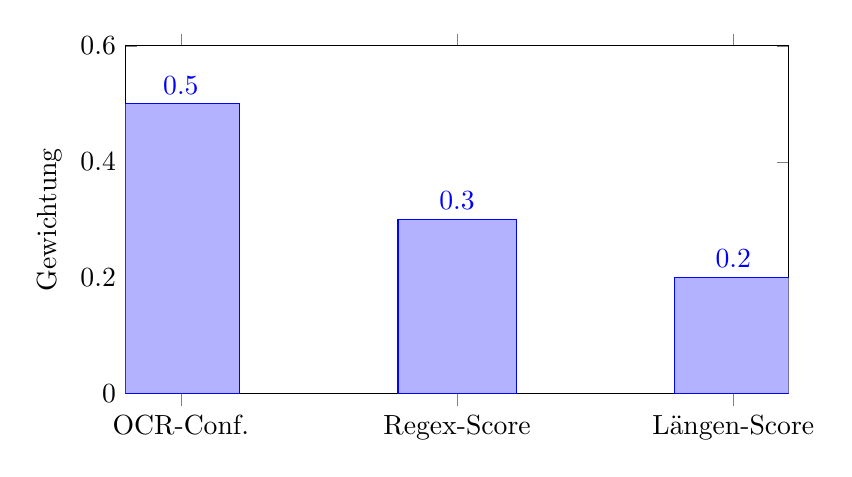
\begin{tikzpicture}
\begin{axis}[
    ybar,
    bar width=1.5cm,
    ylabel={Gewichtung},
    symbolic x coords={OCR-Conf., Regex-Score, Längen-Score},
    xtick=data,
    ymin=0, ymax=0.6,
    nodes near coords,
    nodes near coords align={vertical},
    width=10cm,
    height=6cm
]
\addplot coordinates {(OCR-Conf., 0.5) (Regex-Score, 0.3) (Längen-Score, 0.2)};
\end{axis}
\end{tikzpicture}
\caption{Gewichtung der Komponenten im Konfidenz-Scoring}
\label{fig:Konfidenz_weights}
\end{figure}

Beispiel: Ein Signal-Text \enquote{A12} mit OCR-Konfidenz 1.5, gültiger Regex und erwarteter Länge würde den Score erhalten:
$S_{\text{total}} = 0.5 \cdot 0.75 + 0.3 \cdot 1.0 + 0.2 \cdot 1.0 = 0.875$ (sehr gutes Ergebnis).

\subsubsection{Fehlerbehandlung und Fuzzy-Matching}

Wenn die OCR ein leeres Ergebnis liefert oder der Text keinerlei Zeichen enthält, wird ein Platzhalter-Text generiert: \enquote{UNREADABLE\_} gefolgt von der Symbolklasse (z.B. \enquote{UNREADABLE\_signal}). Dies ermöglicht es, solche Fälle später in der Benutzeroberfläche zu identifizieren und manuell zu korrigieren.

Bei ungültigen Ergebnissen (die das Validierungsmuster nicht erfüllen) wird ein Fuzzy-Matching-Mechanismus aktiviert. Dieser vergleicht den erkannten Text mit einer Liste bekannter korrekter Werte aus früheren Extraktionen. Der Vergleich erfolgt mittels \textbf{Levenshtein-Distanz}, die misst, wie viele Einfüge-, Lösch- oder Ersetzungsoperationen notwendig sind, um einen String in einen anderen zu transformieren.\cite{levenshtein1966}

Beispiele für Levenshtein-Distanz:
\begin{itemize}
    \item \enquote{A12} → \enquote{A1Z}: Distanz = 1 (ein Zeichen ersetzt)
    \item \enquote{A12} → \enquote{A123}: Distanz = 1 (ein Zeichen eingefügt)
    \item \enquote{A12} → \enquote{B34}: Distanz = 3 (alle drei Zeichen ersetzt)
\end{itemize}

Wenn die minimale Levenshtein-Distanz zu einem bekannten Wert kleiner als 2 ist (maximal 2 Änderungen erforderlich), wird dieser bekannte Wert als automatische Korrektur übernommen. Dieser Mechanismus ist besonders hilfreich bei systematischen OCR-Fehlern wie der Verwechslung von:
\begin{itemize}
    \item \enquote{O} (Buchstabe) und \enquote{0} (Ziffer)
    \item \enquote{l} (kleines L) und \enquote{1} (Eins)
    \item \enquote{S} und \enquote{5}
    \item \enquote{B} und \enquote{8}
\end{itemize}

Der Schwellenwert von 2 wurde so gewählt, dass er echte Tippfehler korrigiert, aber keine falschen Korrekturen einführt. Tests zeigten, dass eine Distanz von 3 oder mehr zu oft zu falschen Korrekturen führt.

Falls kein ähnlicher bekannter Wert gefunden wird, wird das ungültige Ergebnis mit dem Präfix \enquote{INVALID\_} markiert (z.B. \enquote{INVALID\_A1Z3X}), um dem Benutzer zu signalisieren, dass hier eine manuelle Überprüfung erforderlich ist.

\subsection{Zusammenfassung der Pipeline-Integration}

Die gesamte OCR-Pipeline wird als modulare Funktion implementiert, die eine Liste von YOLO-Detektionen sowie das Originalbild als Eingabe erhält. Für jede Detektion werden folgende sieben Schritte nacheinander ausgeführt:

\begin{enumerate}
    \item \textbf{Bildausschnitt extrahieren}: Basierend auf den Koordinaten $(x, y)$, der Größe $(w, h)$ und dem Winkel $\theta$ der Bounding Box wird der relevante Bereich aus dem Originalbild ausgeschnitten.
    
    \item \textbf{Klassenspezifisches Preprocessing}: Je nach Symbolklasse werden die entsprechenden Vorverarbeitungsschritte angewendet - adaptive Padding-Berechnung, morphologische Filterung für GKS, oder Multi-Scale-Processing für Koordinaten.
    
    \item \textbf{Dual-Angle Routing}: Basierend auf dem Rotationswinkel wird entweder der Cardinal Path (bei Winkeln $\leq$ $15^\circ$) oder der Angular Path (bei Winkeln >$15^\circ$) gewählt und die entsprechende Transformation (diskrete Rotation oder Perspektiventransformation) durchgeführt.
    
    \item \textbf{Multi-Engine OCR}: Der vorverarbeitete Bildausschnitt wird durch die kaskadierende OCR-Pipeline geschickt. Zuerst PaddleOCR mit vier Rotationen, dann bei Bedarf Tesseract, und optional EasyOCR.
    
    \item \textbf{Post-Processing}: Das OCR-Ergebnis wird bereinigt - führende/nachfolgende Leerzeichen werden entfernt, und die Groß-/Kleinschreibung wird bei Bedarf normalisiert.
    
    \item \textbf{Validierung und Scoring}: Das Ergebnis wird gegen das klassenspezifische Regex-Muster validiert, und der kombinierte Konfidenz-Score wird berechnet.
    
    \item \textbf{Fehlerbehandlung}: Bei ungültigen Ergebnissen wird Fuzzy-Matching mit bekannten Werten versucht. Falls dies fehlschlägt, wird ein entsprechender Platzhalter (INVALID\_ oder UNREADABLE\_) generiert.
\end{enumerate}

Das finale Ergebnis der gesamten OCR-Pipeline ist eine Liste von Tupeln. Jedes Tupel enthält die ursprüngliche YOLO-Detektion, den erkannten Text und die zugehörige Konfidenz. Diese Liste wird an die nachfolgende Komponente weitergereicht - die Symbol-Text-Verknüpfung, die in Abschnitt \ref{sec:intelligentesymboltextverknüpfung} beschrieben wird.


\section{Intelligente Symbol-Text Verknüpfung}
\label{sec:intelligentesymboltextverknüpfung}
Nach der erfolgreichen Detektion von Symbolen durch YOLOv8-OBB und der Extraktion von 
Textinhalten mittels der orientierungsadaptiven OCR-Pipeline besteht die zentrale 
Herausforderung in der korrekten Zuordnung der extrahierten Texte zu ihren zugehörigen 
Symbolen. Diese Verknüpfung ist essenziell für die Generierung semantisch korrekter 
Datensätze aus den Gleisplänen und adressiert die Anforderungen \textbf{FA-006} 
(Fahrtrichtungsdetektion) und \textbf{FA-007} (Symbol-Koordinaten-Verknüpfung).

Die naive Anwendung rein distanzbasierter Proximity-Algorithmen -- bei denen einfach der nächstgelegene Text einem Symbol zugeordnet wird -- führt bei rotierten Symbolen zu systematischen Fehlzuordnungen. Ein Signal, das beispielsweise um $45^\circ$ gedreht ist, besitzt eine eigene lokale Orientierung, und der zugehörige Text befindet sich typischerweise \enquote{unterhalb} des Signals in dessen lokaler Ausrichtung, nicht notwendigerweise in globalen Bildkoordinaten. Die Implementierung muss daher rotationsinvariante Algorithmen einsetzen, die geometrische Transformationen nutzen, um die semantische räumliche Beziehung zwischen Symbolen und Texten korrekt zu erfassen.

\subsection{Rotationsinvariante Koordinatentransformation}
\label{sec:Koordinatentransformation}
\subsubsection{Problemstellung und mathematisches Modell}

Die Herausforderung liegt darin, dass die von YOLO detektierten Symbole beliebige Rotationswinkel $\theta \in [0^\circ, 360^\circ)$ aufweisen können. Die Textpositionen werden in einem globalen kartesischen Koordinatensystem $(x_{\text{global}}, y_{\text{global}})$ angegeben, welches üblicherweise mit der Bildebene übereinstimmt. Für ein rotiertes Symbol ist jedoch die Definition von Richtungen wie \enquote{unterhalb}, \enquote{rechts von} oder \enquote{links von} in globalen Koordinaten nicht mehr sinnvoll.

Zur Lösung dieses Problems wird für jedes Symbol $A$ ein lokales Koordinatensystem eingeführt, dessen Achsen mit der Orientierung des Symbols übereinstimmen. In diesem lokalen System wird die y-Achse parallel zur Längsrichtung des Symbols definiert, sodass die Begriffe \enquote{oberhalb} und \enquote{unterhalb} relativ zur Symbolausrichtung eindeutig werden.

Für ein Symbol $A$ mit Mittelpunkt $\vec{A}_{\text{pos}} = (x_A, y_A)$ und Rotationswinkel $\theta_A$ wird die Position eines Textkandidaten $C$ mit Mittelpunkt $\vec{C}_{\text{pos}} = (x_C, y_C)$ transformiert. Der globale Distanzvektor ist definiert als:

\begin{equation}
\vec{d}_{\text{global}} = \vec{C}_{\text{pos}} - \vec{A}_{\text{pos}} = \begin{pmatrix} dx \\ dy \end{pmatrix} = \begin{pmatrix} x_C - x_A \\ y_C - y_A \end{pmatrix}
\end{equation}

Die Transformation in das lokale Koordinatensystem des Symbols erfolgt durch eine Rotation um den negativen Winkel $-\theta_A$. Die Rotationsmatrix lautet:

\begin{equation}
\mathbf{R}(-\theta_A) = \begin{pmatrix} 
\cos(-\theta_A) & -\sin(-\theta_A) \\ 
\sin(-\theta_A) & \cos(-\theta_A) 
\end{pmatrix}
= \begin{pmatrix} 
\cos(\theta_A) & \sin(\theta_A) \\ 
-\sin(\theta_A) & \cos(\theta_A) 
\end{pmatrix}
\end{equation}

Der transformierte Distanzvektor im lokalen Koordinatensystem ergibt sich zu:

\begin{equation}
\begin{pmatrix} dx_{\text{local}} \\ dy_{\text{local}} \end{pmatrix} 
= \mathbf{R}(-\theta_A) \cdot \begin{pmatrix} dx \\ dy \end{pmatrix}
= \begin{pmatrix} 
dx \cdot \cos(\theta_A) + dy \cdot \sin(\theta_A) \\ 
-dx \cdot \sin(\theta_A) + dy \cdot \cos(\theta_A) 
\end{pmatrix}
\end{equation}

Mit dieser Transformation können nun Richtungsrelationen unabhängig von der globalen Rotation definiert werden:

\begin{itemize}
    \item \textbf{Unterhalb} des Symbols: $dy_{\text{local}} > 0$
    \item \textbf{Oberhalb} des Symbols: $dy_{\text{local}} < 0$
    \item \textbf{Rechts} vom Symbol: $dx_{\text{local}} > 0$
    \item \textbf{Links} vom Symbol: $dx_{\text{local}} < 0$
\end{itemize}

Die euklidische Distanz im lokalen System ist identisch zur Distanz im globalen System, da Rotationen längentreu sind:

\begin{equation}
d_{\text{local}} = \sqrt{dx_{\text{local}}^2 + dy_{\text{local}}^2} = \sqrt{dx^2 + dy^2} = d_{\text{global}}
\end{equation}

\subsubsection{Praktische Berechnung der Koordinatentransformation}

Die Implementierung der Koordinatentransformation erfolgt für jedes Symbol-Text-Paar einzeln. Zunächst werden die globalen Koordinaten des Symbols $(x_A, y_A)$ und des Textkandidaten $(x_C, y_C)$ aus den YOLO- bzw. OCR-Ergebnissen extrahiert. Der Rotationswinkel $\theta_A$ des Symbols liegt ebenfalls aus der YOLO-Detektion vor und muss von Gradmaß in Bogenmaß konvertiert werden. Die Berechnung der lokalen Koordinaten erfolgt dann durch direkte Anwendung der Transformationsgleichung (6.3), wobei die trigonometrischen Funktionen numerisch ausgewertet werden. 


\begin{figure}[H]
\centering
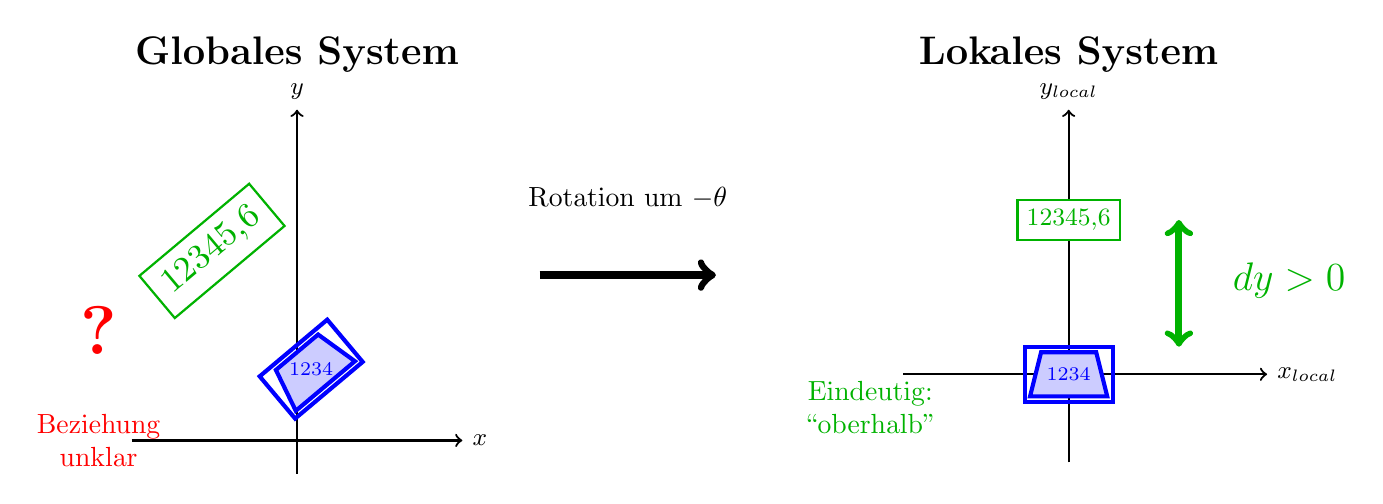
\begin{tikzpicture}[scale=1.4]
    
    % LEFT: Rotated GKS with coordinate - THE PROBLEM
    \begin{scope}
        \node[font=\Large\bfseries] at (0,4) {Globales System};
        
        % Global axes (black, same style as right side)
        \draw[->, black, thick] (-1.5,0.5) -- (1.5,0.5) node[right, font=\small] {$x$};
        \draw[->, black, thick] (0,0.2) -- (0,3.5) node[above, font=\small] {$y$};
        
        % Rotated GKS at angle 40°
        \begin{scope}[shift={(0,1.3)}, rotate=40]
            % Inner trapezoid
            \draw[thick, blue, fill=blue!20, line width=1.5pt] 
                (-0.35,-0.4) -- (-0.25,0) -- (0.25,0) -- (0.35,-0.4) -- cycle;
            % Outer rectangle
            \draw[thick, blue, line width=1.5pt] 
                (-0.4,-0.45) rectangle (0.4,0.05);
            % Number inside
            \node[blue, font=\scriptsize] at (0,-0.2) {1234};
            
            % Coordinate positioned "above" the GKS AND ROTATED with it
            % Need to use 'transform shape' to rotate the node itself
            \node[green!70!black, draw=green!70!black, thick, font=\small, fill=white, 
                  transform shape] 
                 at (0,1.2) {12345,6};
        \end{scope}
        
        % Question mark and label
        \node[red, font=\Huge] at (-1.8,1.5) {\textbf{?}};
        \node[red, font=\normalsize, align=center] at (-1.8,0.5) {Beziehung\\unklar};
    \end{scope}
    
    % ARROW between systems (black, professional, simple)
    \draw[->, line width=1mm, black] (2.2,2) -- (3.8,2);
    \node[black, font=\normalsize, align=center] at (3,2.7) {Rotation um $-\theta$};
    
    % RIGHT: After transformation - THE SOLUTION  
    \begin{scope}[xshift=7cm]
        \node[font=\Large\bfseries] at (0,4) {Lokales System};
        
        % Local coordinate axes (black, same style as left side)
        \draw[->, black, thick] (-1.5,1.1) -- (1.8,1.1) node[right, font=\small] {$x_{\text{local}}$};
        \draw[->, black, thick] (0,0.3) -- (0,3.5) node[above, font=\small] {$y_{\text{local}}$};
        
        % GKS now aligned with local axes (horizontal)
        \begin{scope}[shift={(0,1.3)}]
            % Inner trapezoid
            \draw[thick, blue, fill=blue!20, line width=1.5pt] 
                (-0.35,-0.4) -- (-0.25,0) -- (0.25,0) -- (0.35,-0.4) -- cycle;
            % Outer rectangle
            \draw[thick, blue, line width=1.5pt] 
                (-0.4,-0.45) rectangle (0.4,0.05);
            % Number inside
            \node[blue, font=\scriptsize] at (0,-0.2) {1234};
        \end{scope}
        
        % Coordinate now directly above (in local coordinates, horizontal)
        \node[green!70!black, draw=green!70!black, thick, font=\small, fill=white] 
             at (0,2.5) {12345,6};
        
        % Show the measurement
        \draw[<->, green!70!black, line width=2.5pt] (1.0,1.35) -- (1.0,2.5);
        \node[green!70!black, font=\Large] at (2.0,1.95) {$dy > 0$};
        
        % Checkmark and label
        \node[green!70!black, font=\Huge] at (-1.8,2) {$\checkmark$};
        \node[green!70!black, font=\normalsize, align=center] at (-1.8,0.8) {Eindeutig:\\``oberhalb''};
    \end{scope}
    
\end{tikzpicture}
\caption{Prinzip der rotationsinvarianten Koordinatentransformation}
\label{fig:coordinate_transformation}
\end{figure}

Für jeden Textkandidaten im Umkreis eines Symbols wird diese Transformation durchgeführt, um die räumliche Beziehung in der lokalen Orientierung des Symbols zu bestimmen. Das Ergebnis sind drei Werte: die lokale x-Komponente $dx_{\text{local}}$, die lokale y-Komponente $dy_{\text{local}}$ sowie die euklidische Gesamtdistanz $d_{\text{local}}$. Diese Werte bilden die Grundlage für alle nachfolgenden Verknüpfungsoperationen, da sie eine rotationsinvariante Beschreibung der räumlichen Relation zwischen Symbol und Text ermöglichen.

\subsection{Proximity-basierter Linking-Algorithmus}
\label{subsec:proximity_linking}

\subsubsection{Dynamische Suchbereichsberechnung}

Im Gegensatz zu statischen Suchradien verwendet die Implementierung einen \textit{dimensionsadaptiven} Ansatz, bei dem die Suchbereiche dynamisch aus den Abmessungen der detektierten Bounding Boxes berechnet werden. Dies gewährleistet Robustheit gegenüber unterschiedlichen Symbolgrößen und Planauflösungen.

Für die Verknüpfung eines Ankersymbols (z.B. Signal, GKS-Platte) mit seiner zugehörigen Koordinatenbeschriftung werden die maximalen Suchentfernungen wie folgt berechnet:

\textbf{Vertikaler Suchbereich:}
\begin{equation}
dy_{\text{max}} = 1{,}6 \cdot h_{\text{anchor}} \cdot k_{dy}
\label{eq:dy_max}
\end{equation}

\textbf{Horizontaler Suchbereich:}
\begin{equation}
dx_{\text{max}} = \max\left( k_{dx} \cdot 0{,}6 \cdot \max(w_{\text{anchor}}, w_{\text{coord}}), \; 30 \right)
\label{eq:dx_max}
\end{equation}

wobei $h_{\text{anchor}}$ die Höhe und $w_{\text{anchor}}$ die Breite der Anker-Bounding-Box bezeichnen, $w_{\text{coord}}$ die Breite der Koordinaten-Box, und $k_{dy}$, $k_{dx}$ klassenspezifische Multiplikatoren sind. Der Mindestwert von 30 Pixeln für $dx_{\text{max}}$ stellt sicher, dass auch bei sehr schmalen Symbolen ein ausreichender horizontaler Suchbereich gewährleistet ist.

\subsubsection{Klassenspezifische Multiplikatoren}

Die Multiplikatoren wurden empirisch auf Basis der typischen Layoutkonventionen in Gleisplänen optimiert. Tabelle~\ref{tab:linking_multipliers} zeigt die konfigurierten Werte für alle Symbolklassen.

\begin{table}[H]
\centering
\begin{tabular}{|l|c|c|r|r|c|}
\hline
\textbf{Klasse} & $\boldsymbol{k_{dy}}$ & $\boldsymbol{k_{dx}}$ & \textbf{$dy_{\text{max}}$} & \textbf{$dx_{\text{max}}$} & \textbf{Typ} \\
\hline
\multicolumn{6}{|c|}{\textit{Kernklassen}} \\
\hline
signal & 1.0 & 1.0 & 80--130 px & 30--50 px & Kern \\
gks\_festkodiert & 1.0 & 1.0 & 80--130 px & 30--50 px & Kern \\
gks\_gesteuert & 1.0 & 1.0 & 80--130 px & 30--50 px & Kern \\
gm\_block & 1.0 & 1.0 & 80--130 px & 30--50 px & Kern \\
coordinate & --- & --- & \multicolumn{2}{c|}{(wird verknüpft, nicht Anker)} & Kern \\
\hline
\multicolumn{6}{|c|}{\textit{Auxiliarklassen}} \\
\hline
haltepunkt & 1.0 & 1.0 & 80--130 px & 30--50 px & Auxiliar \\
sverbinder & 1.0 & 1.0 & 80--130 px & 30--50 px & Auxiliar \\
isolierstoß & 1.0 & 1.0 & 80--130 px & 30--50 px & Auxiliar \\
haltetafel & 1.0 & 2.0 & 80--130 px & 60--100 px & Auxiliar \\
prellblock & 1.0 & 2.0 & 80--130 px & 60--100 px & Auxiliar \\
weichenende & 1.0 & 3.0 & 80--130 px & 90--150 px & Auxiliar \\
weichengruppeende & 1.0 & 4.0 & 80--130 px & 120--200 px & Auxiliar \\
\hline
\end{tabular}
\caption{Klassenspezifische Linking-Parameter. Die Wertebereiche für $dy_{\text{max}}$ und $dx_{\text{max}}$ basieren auf typischen Symbolgrößen von 50--80 Pixeln bei 500 DPI.}
\label{tab:linking_multipliers}
\end{table}

Die erhöhten horizontalen Multiplikatoren ($k_{dx} > 1$) für Auxiliarklassen wie \textit{haltetafel}, \textit{prellblock} und \textit{weichengruppeende} reflektieren deren typische Layoutcharakteristik: Diese Symbole haben häufig horizontal versetzte Beschriftungen, während die Kernklassen überwiegend vertikal ausgerichtete Text-Symbol-Relationen aufweisen.

\subsubsection{Spezialfälle mit festen Suchparametern}

Für bestimmte komplexe Verknüpfungsaufgaben, die über die einfache Anker-Koordinaten-Zuordnung hinausgehen, werden feste Pixelwerte verwendet. Diese wurden empirisch auf Basis der bei 500 DPI typischen physikalischen Abstände kalibriert.

\begin{table}[H]
\centering
\small
\begin{tabular}{|l|r|r|p{5.5cm}|}
\hline
\textbf{Anwendungsfall} & \textbf{Parameter} & \textbf{Wert} & \textbf{Beschreibung} \\
\hline
\multicolumn{4}{|c|}{\textit{Fahrtrichtungsdetektion (vgl. Abschnitt~\ref{sec:fahrtrichtung})}} \\
\hline
GKS-Suche & $d_{\text{max}}$ & 250 px & Max. euklidische Distanz zum Signal \\
& $dy_{\text{min}}$ & 30 px & Min. vertikale Separation \\
& $dy_{\text{max}}$ & 200 px & Max. vertikale Separation \\
& $dx_{\text{tol}}$ & $\pm$120 px & Horizontale Toleranz \\
\hline
\multicolumn{4}{|c|}{\textit{Haltetafel-GKS-Fallback}} \\
\hline
GKS-Proximity & $d_{\text{max}}$ & 250 px & Euklidische Distanz zur GKS \\
& $dy_{\text{tol}}$ & 100 px & Max. vertikale Separation \\
& $dx_{\text{tol}}$ & 300 px & Max. horizontale Separation \\
\hline
\multicolumn{4}{|c|}{\textit{Fallback-Mechanismen}} \\
\hline
Isolierstoß & $r_{\text{max}}$ & 300 px & $360^\circ$-Suchradius bei fehlender Zuordnung \\
Gleismittellinie & $d_{\text{ray}}$ & 1500 px & Sicherheitslimit für Ray-Casting \\
\hline
\end{tabular}
\caption{Feste Suchparameter für Spezialfälle (kalibriert für 500 DPI)}
\label{tab:linking_special_params}
\end{table}

\textbf{Physikalische Interpretation:} Bei einer Renderauflösung von 500 DPI entsprechen die Parameter folgenden physikalischen Abständen:
\begin{itemize}
    \item 250 px $\approx$ 12,7 mm (typischer Abstand zwischen Signal und zugehöriger GKS-Platte)
    \item 120 px $\approx$ 6 mm (horizontale Toleranz für leicht versetzte Symbole)
    \item 300 px $\approx$ 15 mm (erweiterter Fallback-Suchbereich)
\end{itemize}

\subsubsection{Richtungsbasierte Filterung}

Neben der Distanzprüfung wird für jede Symbolklasse eine erwartete Richtung definiert, in der sich der zugehörige Text relativ zum Symbol befinden sollte. Die Richtungsbedingungen werden im lokalen Koordinatensystem (vgl. Abschnitt~\ref{sec:Koordinatentransformation}) formuliert:

\begin{itemize}
    \item \textbf{Kernklassen (Signal, GKS, GM-Block):} Text primär \emph{unterhalb} des Symbols erwartet ($dy_{\text{local}} > 0$). Dies entspricht der standardisierten Zeichnungskonvention für Bahnanlagenpläne.
    
    \item \textbf{Auxiliarklassen mit erhöhtem $k_{dx}$:} Flexiblere Richtungstoleranz, da Beschriftungen auch seitlich positioniert sein können ($dy_{\text{local}} > 0$ \textbf{oder} $|dx_{\text{local}}| < dx_{\text{max}}$).
\end{itemize}

Für den Spezialfall der \textit{tight}-Verknüpfung (bei eindeutiger räumlicher Nähe) wird der horizontale Suchbereich reduziert:

\begin{equation}
dx_{\text{max,tight}} = k_{dx} \cdot 0{,}45 \cdot \max(w_{\text{anchor}}, w_{\text{coord}})
\end{equation}

Zusätzlich wird bei aktivierter Linkssuche (\texttt{search\_left=True}) der horizontale Suchbereich asymmetrisch erweitert:

\begin{equation}
dx_{\text{max,left}} = 1{,}3 \cdot dx_{\text{max}} \quad \text{(falls Koordinate links vom Anker)}
\end{equation}

Diese Asymmetrie berücksichtigt, dass in einigen Gleisplänen Koordinatenangaben bevorzugt links von Symbolen platziert werden.

\subsubsection{Algorithmus zur Symbol-Text-Zuordnung}

Der vollständige Linking-Algorithmus kombiniert Distanzprüfung, Richtungsfilterung und Konflikterkennung in einem mehrstufigen Verfahren. Für jedes detektierte Symbol wird zunächst die Menge aller Textkandidaten betrachtet, die sich innerhalb des klassenspezifischen Suchradius befinden. Aus dieser Menge werden diejenigen Kandidaten ausgeschlossen, die nicht der erwarteten Richtungsbedingung genügen. Die verbleibenden Kandidaten werden als potenziell zugehörig betrachtet.

Aus der Menge der gültigen Kandidaten wird derjenige mit der geringsten euklidischen Distanz zum Symbol als beste Zuordnung ausgewählt. Bei Kandidaten mit sehr ähnlichen Distanzen (Differenz kleiner als 5 Pixel) wird zusätzlich die OCR-Konfidenz berücksichtigt: Der Kandidat mit höherer Erkennungssicherheit wird bevorzugt. Dies stellt sicher, dass bei räumlich ambigen Situationen die Qualität der Texterkennung als Entscheidungskriterium herangezogen wird.

Falls für ein Symbol keine Textkandidaten die Filterkriterien erfüllen, bleibt das Symbol zunächst ohne Textzuordnung. In diesem Fall kann im nächsten Schritt der adaptive Lernmechanismus aktiviert werden, um eine Zuordnung basierend auf statistischen Mustern zu versuchen. Symbole, für die auch nach allen Verknüpfungsversuchen kein Text zugeordnet werden konnte, werden im Validierungsdialog der Benutzeroberfläche zur manuellen Überprüfung gekennzeichnet.

\subsection{Adaptive Learning Mechanismus}
\label{subsec:adaptivelearningmechanism}
\subsubsection{Motivation und Konzept}

Obwohl technische Zeichnungen üblicherweise Konventionen folgen, existieren in der Praxis Variationen zwischen verschiedenen Planversionen, Zeichnern oder historischen Perioden. Ein statisches Regelwerk mit festen Suchradien und Richtungen kann in solchen Fällen suboptimal sein. Aus diesem Grund implementiert das System einen adaptiven Lernmechanismus, der erfolgreiche Verknüpfungen analysiert und statistische Muster extrahiert, um die Linking-Parameter dynamisch anzupassen.

Der Mechanismus basiert auf der Beobachtung, dass innerhalb eines einzelnen Gleisplans die Positionierung von Texten relativ zu Symbolen oft konsistent ist. Wenn beispielsweise alle Signalbezeichnungen systematisch 10 Pixel rechts und 20 Pixel unterhalb der Signalsymbole platziert sind, kann das System dieses Muster lernen und für nachfolgende unsichere Fälle nutzen.

\subsubsection{Pattern-Erfassung und statistische Auswertung}

Jede erfolgreiche Symbol-Text-Verknüpfung, die eine definierte Konfidenz-Schwelle überschreitet (typischerweise OCR-Konfidenz $> 0.85$ und eindeutige Regex-Validierung), wird als \enquote{validated link} betrachtet und zur statistischen Auswertung herangezogen. Für diese Links werden die lokalen Offset-Vektoren $(dx_{\text{local}}, dy_{\text{local}})$ persistiert und klassenweise aggregiert.

Das System verwaltet für jede Symbolklasse eine Sammlung von Offset-Vektoren sowie deren statistische Kenngrößen. Zu den gespeicherten Informationen gehören die Liste aller beobachteten Offsets, der Erwartungswert des Offsets, die Standardabweichung sowie die Anzahl der zugrundeliegenden Beobachtungen und der Zeitstempel der letzten Aktualisierung.

Für jede Symbolklasse werden folgende statistische Kenngrößen kontinuierlich aktualisiert. Der Erwartungswert des Offsets $(\mu_x, \mu_y)$ wird als arithmetisches Mittel aller beobachteten Offsets berechnet:

\begin{equation}
\mu_x = \frac{1}{N} \sum_{i=1}^{N} dx_i, \quad \mu_y = \frac{1}{N} \sum_{i=1}^{N} dy_i
\end{equation}

wobei $N$ die Anzahl der validierten Links für die entsprechende Klasse bezeichnet. Die Standardabweichung $(\sigma_x, \sigma_y)$ quantifiziert die Streuung der Offsets und wird berechnet als:

\begin{equation}
\sigma_x = \sqrt{\frac{1}{N-1} \sum_{i=1}^{N} (dx_i - \mu_x)^2}, \quad \sigma_y = \sqrt{\frac{1}{N-1} \sum_{i=1}^{N} (dy_i - \mu_y)^2}
\end{equation}

Die Verwendung der Stichprobenstandardabweichung (Division durch $N-1$ statt $N$) liefert einen erwartungstreuen Schätzer für die Populationsvarianz. Ein Minimum von $N \geq 10$ wird gefordert, bevor die statistischen Kenngrößen als hinreichend zuverlässig für prädiktive Zwecke betrachtet werden. Diese Schwelle stellt sicher, dass die Schätzungen der Verteilungsparameter nicht durch einzelne Ausreißer dominiert werden.

\subsubsection{Probabilistische Fenstersuche}

Wenn für ein Symbol keine Textkandidaten im Standard-Suchradius gefunden werden, wird die probabilistische Fenstersuche aktiviert, sofern für die entsprechende Symbolklasse ausreichend gelernte Patterns vorliegen. Dieses Verfahren nutzt die statistischen Kenngrößen aus den zuvor erfassten erfolgreichen Verknüpfungen, um eine erwartete Position für den fehlenden Text zu berechnen und dort gezielt zu suchen.

Die erwartete Position des Textes im globalen Koordinatensystem wird durch Rücktransformation des mittleren lokalen Offsets berechnet. Zunächst wird der in den Pattern-Statistiken gespeicherte mittlere Offset $(\mu_x, \mu_y)$ aus dem lokalen Koordinatensystem des Symbols zurück ins globale System transformiert. Dies erfolgt durch Anwendung der inversen Rotation, also durch Rotation um den positiven Winkel $+\theta_A$:

\begin{equation}
\begin{pmatrix} \Delta x_{\text{global}} \\ \Delta y_{\text{global}} \end{pmatrix}
= \begin{pmatrix} 
\cos(\theta_A) & -\sin(\theta_A) \\ 
\sin(\theta_A) & \cos(\theta_A) 
\end{pmatrix}
\cdot
\begin{pmatrix} \mu_x \\ \mu_y \end{pmatrix}
\end{equation}

Die erwartete globale Position des Textes ergibt sich dann durch Addition dieses transformierten Offsets zur Symbolposition:

\begin{equation}
\vec{C}_{\text{expected}} = \begin{pmatrix} x_{\text{expected}} \\ y_{\text{expected}} \end{pmatrix} 
= \begin{pmatrix} x_A \\ y_A \end{pmatrix} + \begin{pmatrix} \Delta x_{\text{global}} \\ \Delta y_{\text{global}} \end{pmatrix}
\end{equation}

Um die erwartete Position herum wird ein achsenparalleles Suchfenster definiert, dessen Ausdehnung durch die Standardabweichungen der gelernten Offset-Verteilung bestimmt wird. Das Suchfenster wird so gewählt, dass es einem zweifachen der Standardabweichung in jeder Koordinatenrichtung entspricht. Dies entspricht bei Annahme einer Normalverteilung einem Konfidenzintervall von ca. 95\%, d.h. die meisten tatsächlichen Textpositionen sollten innerhalb dieses Fensters liegen:

\begin{equation}
\text{Suchfenster}: \quad |x - x_{\text{expected}}| \leq 2\sigma_x, \quad |y - y_{\text{expected}}| \leq 2\sigma_y
\end{equation}

Alle Textkandidaten, deren Positionen innerhalb dieses Fensters liegen, werden als potenzielle Zuordnungen betrachtet. Aus dieser gefilterten Menge wird der zur erwarteten Position $\vec{C}_{\text{expected}}$ nächstgelegene Kandidat ausgewählt. Die Distanz wird dabei als euklidische Distanz zur erwarteten Position berechnet, nicht zur Symbolposition, da die erwartete Position die durch das Lernen verfeinerte beste Schätzung der Textlage darstellt.
Abbildung \ref{fig:adaptive_window} illustriert dieses Verfahren: Ausgehend vom Signal wird die erwartete Textposition durch den mittleren gelernten Offset bestimmt (roter Punkt). Das Suchfenster (rot gestrichelt) umfasst einen $2\sigma$ Bereich um diese Position. Nur Textkandidaten innerhalb dieses Fensters (grün) werden für die Zuordnung berücksichtigt, während außenliegende Kandidaten (schwarz) ignoriert werden
Die probabilistische Fenstersuche wird nur dann aktiviert, wenn mindestens 10 validierte Links für die entsprechende Symbolklasse vorliegen. Dies stellt sicher, dass die statistischen Schätzer eine ausreichende Präzision besitzen. Für seltene Symbolklassen oder zu Beginn der Verarbeitung, wenn noch wenige Links validiert wurden, greift das System auf die konventionelle Proximity-Suche zurück.

\begin{figure}[H]
\centering
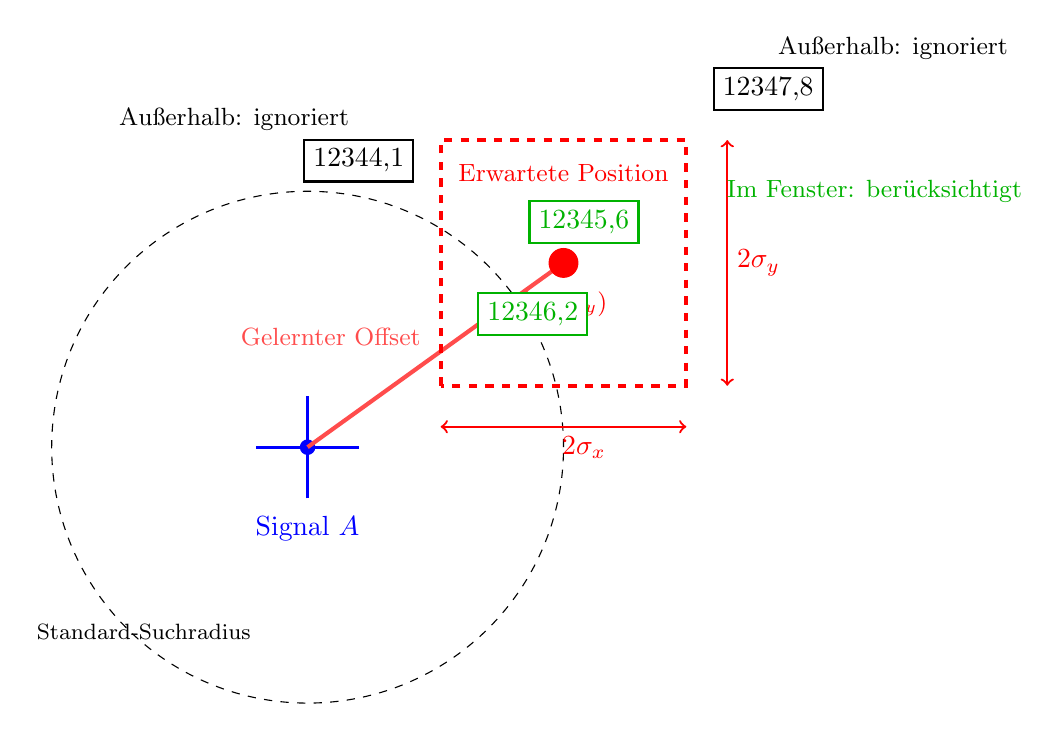
\begin{tikzpicture}[scale=1.3]

    % Signal at origin
    \draw[very thick, blue] (-0.5,0) -- (0.5,0);
    \draw[very thick, blue] (0,-0.5) -- (0,0.5);
    \filldraw[blue] (0,0) circle (2pt);
    \node[blue, font=\normalsize] at (0,-0.8) {Signal $A$};
    
    % Standard search radius (very faint, for context only)
    \draw[dashed, black, thin] (0,0) circle (2.5);
    \node[black, font=\footnotesize] at (-1.6,-1.8) {Standard-Suchradius};
    
    % Learned offset vector
    \draw[->, very thick, red!70, line width=1.5pt] (0,0) -- (2.5,1.8);
    \node[red!70, font=\small, anchor=south east] at (1.2,0.9) {Gelernter Offset};
    
    % Expected position
    \filldraw[red] (2.5,1.8) circle (4pt);
    \node[red, font=\small, anchor=south] at (2.5,2.5) {Erwartete Position};
    \node[red, font=\small] at (2.5,1.4) {$(\mu_x, \mu_y)$};
    
    % Probabilistic window (larger, clearer)
    \draw[very thick, red, dashed, line width=1.5pt] (1.3,0.6) rectangle (3.7,3.0);
    
    % Window dimensions - placed outside, clearer
    \draw[<->, red, thick] (1.3,0.2) -- (3.7,0.2);
    \node[red, font=\normalsize, below] at (2.7,0.2) {$2\sigma_x$};
    
    \draw[<->, red, thick] (4.1,0.6) -- (4.1,3.0);
    \node[red, font=\normalsize, right] at (4.1,1.8) {$2\sigma_y$};
    
    % Text candidates INSIDE window (green box, black text, no dots)
    \node[green!70!black, draw=green!70!black, thick, fill=white, font=\normalsize] 
         at (2.7,2.2) {12345,6};
    
    \node[green!70!black, draw=green!70!black, thick, fill=white, font=\normalsize] 
         at (2.2,1.3) {12346,2};
    
    % Label for inside candidates
    \node[green!70!black, font=\small, anchor=west] at (4.0,2.5) {Im Fenster: berücksichtigt};
    
    % Text candidates OUTSIDE window (black box, black text, no dots)
    \node[black, draw=black, thick, fill=white, font=\normalsize] 
         at (4.5,3.5) {12347,8};
    
    \node[black, draw=black, thick, fill=white, font=\normalsize] 
         at (0.5,2.8) {12344,1};
    
    % Label for outside candidates (black)
    \node[black, font=\small, anchor=west] at (4.5,3.9) {Außerhalb: ignoriert};
    \node[black, font=\small, anchor=east] at (0.5,3.2) {Außerhalb: ignoriert};
    
\end{tikzpicture}
\caption{Probabilistische Fenstersuche basierend auf gelernten Offset-Patterns}
\label{fig:adaptive_window}
\end{figure}

Dieser adaptive Mechanismus ermöglicht es dem System, sich an plan-spezifische Layoutkonventionen anzupassen. Insbesondere bei historischen Plänen oder Zeichnungen von verschiedenen Bearbeitern, die von modernen Standardkonventionen abweichen, verbessert der Lernmechanismus die Linking-Rate signifikant. Empirisch zeigt sich eine Verbesserung der erfolgreichen Zuordnungen um ca. 12\% gegenüber rein statischen Regeln, insbesondere bei inkonsistenten oder nicht-standardkonformen Layouts.

\subsection{Komplexe Verknüpfungslogik für Spezialfälle}

\subsubsection{Fahrtrichtungsdetektion}
\label{sec:fahrtrichtung}

In Gleisplänen ist die Fahrtrichtung eines Signals ein kritisches Attribut, das angibt, in welche Richtung das Signal wirkt und für welche Fahrtrichtung es relevant ist. Die konventionelle Kodierung sieht zwei mögliche Fahrtrichtungen vor: Richtung A entspricht üblicherweise der Fahrt in positiver Streckenrichtung, Richtung B der Fahrt in negativer Streckenrichtung. 

Anstatt die Fahrtrichtung als separate Klassifikationsaufgabe zu behandeln, wird sie im implementierten System durch geometrische Analyse der räumlichen Beziehung zwischen Signal und zugeordneter GKS(festkodiert) bestimmt. Diese Methode nutzt die in Gleisplänen übliche Konvention, dass die relative Position der GKS(festkodiert) zum Signal die Fahrtrichtung kodiert.

Die Fahrtrichtung wird durch die Vorzeichenbetrachtung der lokalen y-Koordinate der GKS(festkodiert) relativ zum Signal bestimmt. Hierbei wird die in Abschnitt \ref{sec:Koordinatentransformation} beschriebene Koordinatentransformation angewendet, um die Position der GKS(festkodiert) im lokalen Koordinatensystem des Signals zu ermitteln. Die Entscheidungsregel lautet:

\begin{equation}
\text{Fahrtrichtung} = \begin{cases} 
\text{A} & \text{falls } dy_{\text{local}}(\text{GKS}, \text{Signal}) < 0 \\
\text{B} & \text{falls } dy_{\text{local}}(\text{GKS}, \text{Signal}) > 0
\end{cases}
\end{equation}

Eine negative lokale y-Koordinate bedeutet, dass die GKS sich oberhalb des Signals in dessen lokaler Orientierung befindet, was nach Konvention der Fahrtrichtung A entspricht. Eine positive lokale y-Koordinate indiziert, dass die GKS unterhalb des Signals liegt, was der Fahrtrichtung B zugeordnet wird. Abbildung~\ref{fig:signal_direction} veranschaulicht diese Bestimmung durch die relative Position der zugeordneten GKS im lokalen Koordinatensystem. Die Koordinatenangabe befindet sich zwischen Signal und GKS. Links ist der Fall $dy_{\text{local}} < 0$ (GKS oberhalb) dargestellt, was Fahrtrichtung~A entspricht; rechts der Fall $dy_{\text{local}} > 0$ (GKS unterhalb), entsprechend Fahrtrichtung~B.
\begin{figure}[H]
\centering
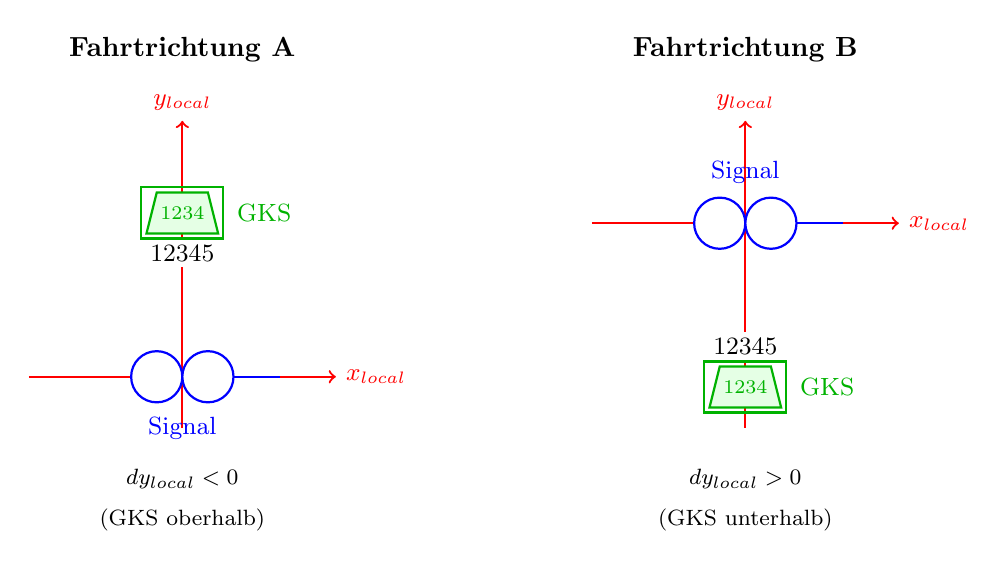
\begin{tikzpicture}[scale=1.3]
    % --- LINKE SEITE (Fahrtrichtung A) ---
    \begin{scope}
        \node at (0,3.2) {\textbf{Fahrtrichtung A}};
        
        % Achsen (werden zuerst gezeichnet -> liegen hinten)
        \draw[->, red, thick] (-1.5,0) -- (1.5,0) node[right, font=\small] {$x_{\text{local}}$};
        \draw[->, red, thick] (0,-0.5) -- (0,2.5) node[above, font=\small] {$y_{\text{local}}$};
        
        % Signal (bei 0,0)
        \begin{scope}[shift={(0,0)}]
            \draw[thick, blue, fill=white] (-0.25,0) circle (0.25);
            \draw[thick, blue, fill=white] (0.25,0) circle (0.25);
            \draw[thick, blue] (0.50,0) -- (0.95,0);
        \end{scope}
        \node[blue, font=\small] at (0,-0.5) {Signal};
        
        % Koordinate (Box entfernt, fill=white verdeckt die Linie dahinter)
        \node[fill=white, font=\small, inner sep=2pt] at (0,1.2) {12345};
        
        % GKS (oberhalb)
        \begin{scope}[shift={(0,1.4)}]
            \draw[thick, green!70!black, fill=green!10] 
                (-0.35,0) -- (-0.25,0.4) -- (0.25,0.4) -- (0.35,0) -- cycle;
            \draw[thick, green!70!black] 
                (-0.4,-0.05) rectangle (0.4,0.45);
            \node[green!70!black, font=\scriptsize] at (0,0.2) {1234};
        \end{scope}
        \node[green!70!black, font=\small] at (0.8,1.6) {GKS};
        
        \node[font=\footnotesize] at (0,-1.0) {$dy_{\text{local}} < 0$};
        \node[font=\footnotesize] at (0,-1.4) {(GKS oberhalb)};
    \end{scope}
    
    % --- RECHTE SEITE (Fahrtrichtung B) ---
    \begin{scope}[xshift=5.5cm]
        \node at (0,3.2) {\textbf{Fahrtrichtung B}};
        
        % Offset (Symmetrie nach oben geschoben)
        \def\yoff{1.5} 
        
        % Achsen
        \draw[->, red, thick] (-1.5,\yoff) -- (1.5,\yoff) node[right, font=\small] {$x_{\text{local}}$};
        \draw[->, red, thick] (0,-0.5) -- (0,2.5) node[above, font=\small] {$y_{\text{local}}$};
        
        % Signal (bei y = 1.5)
        \begin{scope}[shift={(0,\yoff)}]
            \draw[thick, blue, fill=white] (-0.25,0) circle (0.25);
            \draw[thick, blue, fill=white] (0.25,0) circle (0.25);
            \draw[thick, blue] (0.50,0) -- (0.95,0);
        \end{scope}
        \node[blue, font=\small] at (0,\yoff+0.5) {Signal};
        
        % Koordinate (Box weg, Linie verdeckt)
        \node[fill=white, font=\small, inner sep=2pt] at (0,\yoff-1.2) {12345};
        
        % GKS unterhalb
        \begin{scope}[shift={(0,\yoff-1.4)}]
            \draw[thick, green!70!black, fill=green!10] 
                (-0.35,-0.4) -- (-0.25,0) -- (0.25,0) -- (0.35,-0.4) -- cycle;
            \draw[thick, green!70!black] 
                (-0.4,-0.45) rectangle (0.4,0.05);
            \node[green!70!black, font=\scriptsize] at (0,-0.2) {1234};
        \end{scope}
        \node[green!70!black, font=\small] at (0.8,\yoff-1.6) {GKS};
        
        % Annotation
        \node[font=\footnotesize] at (0,-1.0) {$dy_{\text{local}} > 0$};
        \node[font=\footnotesize] at (0,-1.4) {(GKS unterhalb)};
    \end{scope}
    
\end{tikzpicture}
\caption{Geometrische Bestimmung der Fahrtrichtung eines Signals}
\label{fig:signal_direction}
\end{figure}
Die konkreten Suchparameter für die GKS-Lokalisierung sind in Tabelle~\ref{tab:linking_special_params} dokumentiert: Die maximale Suchdistanz beträgt 250 Pixel ($\approx$ 12,7 mm bei 500 DPI), wobei die vertikale Separation zwischen 30 und 200 Pixeln liegen muss und eine horizontale Toleranz von $\pm$120 Pixeln erlaubt ist.
Diese geometrische Ableitung der Fahrtrichtung hat mehrere Vorteile gegenüber einer expliziten Klassifikation. Erstens wird kein separater Klassifikator benötigt, der auf Trainingsbeispielen für Fahrtrichtungen trainiert werden müsste. Zweitens ist die Methode robust gegenüber verschiedenen graphischen Darstellungsformen von Signalen, da sie ausschließlich auf der räumlichen Anordnung basiert und nicht auf visuellen Merkmalen des Symbols selbst. Drittens ist die Bestimmung rotationsinvariant, da sie im lokalen Koordinatensystem des Signals operiert.

\subsubsection{Haltepunkt-Gruppierung}

Ein Haltepunkt in einem Gleisplan ist eine komplexe Entität, die aus drei separaten Komponenten besteht, die räumlich assoziiert werden müssen. Die erste Komponente ist das Haltepunkt-Symbol selbst, welches die Position des Haltepunkts im Plan markiert. Die zweite Komponente ist das zugeordnete Signal, das den Haltepunkt absichert und den Zügen das Halt-Gebot signalisiert. Die dritte Komponente ist die Koordinatenangabe, typischerweise in Form einer Kilometerangabe, die den Haltepunkt auf der Strecke verortet.

Die korrekte Gruppierung dieser drei Elemente ist essentiell für die semantische Interpretation des Haltepunkts. Die geometrische Bedingung, die zur Identifikation zusammengehöriger Elemente herangezogen wird, basiert auf der Beobachtung, dass die Koordinate sich räumlich zwischen dem Haltepunkt-Symbol und dem zugeordneten Signal befinden sollte. Dies reflektiert die übliche Zeichnungskonvention, bei der die Kilometerangabe des Haltepunkts in der Nähe des Haltepunkt-Symbols angebracht wird, während das Signal etwas weiter entfernt positioniert ist.

Die Implementierung dieser geometrischen Bedingung erfolgt durch einen approximativen Kollinearitätstest. Für drei Punkte H (Haltepunkt-Symbol), K (Koordinate) und S (Signal) wird geprüft, ob K näherungsweise auf der Verbindungslinie zwischen H und S liegt. Exakte Kollinearität würde bedeuten, dass die Summe der Teilstrecken $d(H, K) + d(K, S)$ exakt gleich der direkten Distanz $d(H, S)$ ist. In der Praxis wird eine Toleranz $\epsilon$ eingeführt, um kleine Abweichungen von der perfekten Kollinearität zu erlauben:

\begin{equation}
d(H, K) + d(K, S) \leq d(H, S) + \epsilon
\end{equation}

wobei $d(\cdot, \cdot)$ die euklidische Distanz zwischen zwei Punkten bezeichnet. Die Toleranz $\epsilon$ wird typischerweise auf 20 Pixel gesetzt, um eine gewisse Flexibilität gegenüber nicht-perfekt linearen Anordnungen zu ermöglichen, gleichzeitig aber sicherzustellen, dass die Koordinate tatsächlich zwischen den beiden anderen Elementen liegt und nicht deutlich von der Verbindungslinie abweicht.

Der Gruppierungsalgorithmus iteriert über alle detektierten Haltepunkt-Symbole. Für jedes Haltepunkt-Symbol werden alle Signale und Koordinaten innerhalb eines definierten Umkreises (typischerweise 250 Pixeln) als potenzielle Gruppierungspartner betrachtet. Für jede Kombination aus Haltepunkt, Signal und Koordinate wird die Kollinearitätsbedingung geprüft. Die erste Kombination, die die Bedingung erfüllt, wird als gültige Gruppierung akzeptiert und persistiert.

Diese geometrische Gruppierungsmethode stellt sicher, dass die semantisch zusammengehörigen Elemente eines Haltepunkts korrekt identifiziert werden. In der exportierten Datenstruktur werden gruppierte Haltepunkte als zusammenhängende Einheiten behandelt, wobei alle drei Komponenten miteinander verlinkt sind. Dies ermöglicht es nachgelagerten Systemen oder menschlichen Anwendern, die vollständige Information eines Haltepunkts effizient abzurufen, ohne die drei Komponenten manuell zusammensuchen zu müssen.

\subsection{Zusammenfassung der Verknüpfungslogik}

Die implementierte Symbol-Text-Verknüpfung kombiniert mehrere komplementäre Ansätze:

\begin{enumerate}
    \item \textbf{Rotationsinvariante Geometrie}: Transformation in lokale Koordinatensysteme ermöglicht richtungsbasierte Filterung unabhängig von der globalen Orientierung.
    
    \item \textbf{Dimensionsadaptive Suchbereiche}: Dynamische Berechnung der Suchparameter aus Bounding-Box-Dimensionen (Gleichungen~\ref{eq:dy_max} und \ref{eq:dx_max}) mit klassenspezifischen Multiplikatoren gewährleistet Robustheit gegenüber unterschiedlichen Symbolgrößen und Planauflösungen.
    
    \item \textbf{Adaptive Lernmechanismen}: Statistische Analyse erfolgreicher Links ermöglicht Anpassung an plan-spezifische Layouts.
    
    \item \textbf{Komplexe Relationserkennung}: Spezielle Algorithmen für Fahrtrichtungsdetektion und Haltepunkt-Gruppierung behandeln semantisch reiche Objektbeziehungen.
\end{enumerate}

Die Kombination dieser Techniken erreicht eine hohe Linking-Genauigkeit, die in Kapitel~\ref{chap:evaluation} quantitativ evaluiert wird.


\section{Datenvalidierung und Qualitätssicherung}
\label{sec:validierungundsicherung}
Die Validierung extrahierter Daten stellt einen kritischen Schritt zur Sicherstellung 
der Datenqualität dar. Das implementierte System kombiniert regelbasierte Validierung 
mit intelligenten Korrekturvorschlägen und adressiert damit die Anforderungen 
\textbf{FA-008} (manuelle Korrektur durch Human-in-the-Loop), \textbf{NFA-004} 
(Robustheit gegenüber fehlerhaften Eingaben) und \textbf{NFA-005} (Prüfbarkeit 
durch strukturierte Fehlerberichte).

\subsection{Validierungsarchitektur}

\subsubsection{Grundstruktur des Validierungsframeworks}
Die Validierungsarchitektur basiert auf einem modularen Framework, das die extrahierten Daten in tabellarischer Form entgegennimmt und eine strukturierte Fehleranalyse durchführt. Das zentrale Validierungsmodul prüft dabei einen DataFrame, der alle Erkennungen aus der YOLO-Pipeline, die zugehörigen OCR-Texte sowie die durch das Linking-Modul hergestellten Verknüpfungen enthält. Die Ausgabe der Validierung besteht aus einer Liste von Validierungsproblemen, wobei jedes Problem durch mehrere Attribute charakterisiert wird.

Ein Validierungsproblem wird durch folgende Eigenschaften beschrieben. Der Schweregrad klassifiziert das Problem in die Kategorien Fehler, Warnung oder Information, wobei Fehler kritische Inkonsistenzen darstellen, die zwingend einer Korrektur bedürfen, während Warnungen auf potenzielle Probleme hinweisen, die einer Überprüfung bedürfen. Die Kategorie beschreibt die Art des Problems, beispielsweise Formatfehler, Duplikate oder fehlende Daten. Das betroffene Feld identifiziert die spezifische Datenspalte, in der das Problem auftritt. Bei automatisch korrigierbaren Problemen wird zusätzlich ein Korrekturvorschlag mit dem empfohlenen neuen Wert bereitgestellt. Die Konfidenz des Korrekturvorschlags wird als normalisierter Wert im Intervall $[0, 1]$ angegeben, wobei höhere Werte eine größere Zuverlässigkeit der vorgeschlagenen Korrektur indizieren.

Die Validierung erfolgt durch sequenzielle Ausführung aller implementierten Prüfungen, wobei das Ergebnis die Gesamtheit aller identifizierten Probleme sowie statistische Kennzahlen zur Fehlerverteilung umfasst. Diese strukturierte Repräsentation ermöglicht sowohl die programmatische Weiterverarbeitung als auch die Präsentation in einer benutzerfreundlichen Oberfläche.
\textbf{Validierungsfokus:} Die regelbasierte Validierung konzentriert sich primär auf 
die fünf Kernklassen, da diese für den produktiven Einsatz bei Siemens Mobility 
relevant sind. Für Auxiliarklassen werden grundlegende Formatprüfungen durchgeführt, 
jedoch keine domänenspezifischen Plausibilitätsprüfungen.
\subsubsection{Dreistufige Validierungsstrategie}

Die Validierung ist hierarchisch in drei Ebenen organisiert, die aufeinander aufbauen und unterschiedliche Aspekte der Datenqualität adressieren. Diese Strukturierung ermöglicht eine systematische Fehleridentifikation von grundlegenden Formatproblemen bis hin zu komplexen semantischen Inkonsistenzen.

\begin{figure}[H]
    \centering
    % --- HIER IST DIE ÄNDERUNG ---
    % Ein horizontaler Abstand von 1.5cm schiebt das Bild nach rechts.
    % Passe den Wert an (z.B. 1cm, 2.5cm), bis es perfekt sitzt.
    \hspace*{1.5cm} 
    % -----------------------------
    \begin{tikzpicture}[
        node distance=1.5cm,
        box/.style={rectangle, draw, minimum width=6cm, minimum height=1cm, align=center, fill=blue!10},
        layer/.style={rectangle, draw, minimum width=7cm, minimum height=1.5cm, align=center, fill=green!10, rounded corners},
        arrow/.style={->, >=stealth, thick}
    ]

    % Input
    \node[box] (input) {DataFrame\\(YOLO + OCR + Linking)};

    % Layer 1
    \node[layer, below=of input] (layer1) {
        \textbf{Ebene 1: Syntaktische Validierung}\\
        Regex-Patterns pro Klasse
    };

    % Layer 2
    \node[layer, below=of layer1] (layer2) {
        \textbf{Ebene 2: Semantische Validierung}\\
        Wertebereich, Konsistenzprüfung
    };

    % Layer 3
    \node[layer, below=of layer2] (layer3) {
        \textbf{Ebene 3: Räumliche Validierung}\\
        Proximity, Duplikate, YOLO-Konfidenz
    };

    % Output
    \node[box, below=of layer3, fill=orange!10] (output) {ValidationIssue Liste\\(Fehler, Warnungen, Hinweise)};

    % Arrows
    \draw[arrow] (input) -- (layer1);
    \draw[arrow] (layer1) -- (layer2);
    \draw[arrow] (layer2) -- (layer3);
    \draw[arrow] (layer3) -- (output);

    % Side annotations
    \node[right=1.5cm of layer1, text width=3cm, font=\small] {Format-\\korrektheit};
    \node[right=1.5cm of layer2, text width=3cm, font=\small] {Inhaltliche\\Plausibilität};
    \node[right=1.5cm of layer3, text width=3cm, font=\small] {Geometrische\\Beziehungen};

    \end{tikzpicture}
    \caption{Dreistufige Validierungsarchitektur mit hierarchischer Fehleranalyse}
    \label{fig:validation_architecture}
\end{figure}

Die erste Ebene, die syntaktische Validierung, prüft die formale Korrektheit der extrahierten Texte anhand klassenspezifischer Muster. Für jede Objektklasse wurde ein regulärer Ausdruck definiert, der das erwartete Textformat beschreibt. Diese Muster basieren auf der Analyse realer Gleispläne und den geltenden Standards für Signalbezeichnungen und Kilometrierungen.

Für Signalbezeichnungen wird das Muster durch den regulären Ausdruck beschrieben, der eine bis vier Großbuchstaben (einschließlich deutscher Umlaute Ä, Ö, Ü) gefolgt von einer bis vier Ziffern erwartet. Das entsprechende Regex-Muster lautet: ein bis vier Zeichen aus der Menge A bis Z sowie Ä, Ö, Ü, gefolgt von einer bis vier Ziffern. Dieses Format entspricht der standardisierten Signalnomenklatur, bei der Buchstaben den Signaltyp oder die Streckenbezeichnung kodieren, während Ziffern die spezifische Signalnummer angeben. Beispiele für gültige Signalbezeichnungen sind somit A101, BHR201 oder F3a.

Für GKS-Platten (Gleiskontakte) gilt ein numerisches Format mit drei bis vier Ziffern. GKS-Platten werden ausschließlich durch diese Ziffernfolgen identifiziert, beispielsweise 1234 oder 567.

Die Validierung von Koordinatentexten erfolgt mehrstufig, da Koordinatenangaben sowohl einen numerischen Teil als auch optionale Zusatzinformationen enthalten können. Der numerische Hauptteil besteht aus einer bis drei Ziffern, gefolgt von einem Dezimaltrenner (Punkt oder Komma), gefolgt von drei bis vier Ziffern. Dies berücksichtigt unterschiedliche Schreibweisen in verschiedenen Dokumentversionen. Zusätzlich wird geprüft, dass keine Kleinbuchstaben im Text vorkommen, mit Ausnahme der standardisierten Abkürzung Gl für Gleis. Ebenfalls wird validiert, dass zwischen den Ziffern keine Buchstaben eingefügt sind, da dies auf OCR-Fehler hinweist. Bei Koordinaten mit Gleisangaben wird zudem die korrekte Klammerung geprüft, sodass Angaben wie 10.5123(Gl.1) als gültig erkannt werden, während fehlerhafte Klammerungen wie 10.5123(Gl.1 als problematisch gekennzeichnet werden.

Für die Fahrtrichtungsangabe bei Signalen gilt das restriktive Muster, das ausschließlich die beiden Werte A und B zulässt, entsprechend der binären Richtungskodierung im Eisenbahnwesen.

Die zweite Ebene, die semantische Validierung, überprüft die inhaltliche Plausibilität der extrahierten Werte über die reine Formatprüfung hinaus. Koordinatenwerte werden auf einen plausiblen Wertebereich geprüft, wobei Kilometrierungen im Intervall $[0, 300]$ erwartet werden, da dies dem typischen Streckenbereich deutscher Bahnstrecken entspricht. Werte außerhalb dieses Bereichs werden als potenzielle OCR-Fehler gekennzeichnet.

Bei mehrfach vorkommenden Signalen wird die Konsistenz der zugeordneten Attribute überprüft. Ein Signal mit identischer Bezeichnung sollte in allen Instanzen dieselbe Kilometrierung aufweisen, da physisch identische Signale an einem festen geografischen Punkt lokalisiert sind. Ebenso wird die Konsistenz der Fahrtrichtung geprüft, wobei Inkonsistenzen auf Erkennungsfehler oder tatsächliche Duplikate hindeuten können.

Die dritte Ebene, die räumliche Validierung, analysiert die geometrischen Beziehungen zwischen den erkannten Objekten. Für Objektklassen, die zwingend eine Kilometrierung benötigen wie Signale, GKS-Platten, Weichenblöcke und Streckentrenner wird geprüft, ob eine Koordinate in räumlicher Nähe vorhanden ist. Die Definition räumlicher Nähe erfolgt klassenspezifisch gemäß den in Abschnitt~\ref{subsec:proximity_linking} definierten dynamischen Suchbereichen. Für die Kernklassen (Signal, GKS, GM-Block) resultiert dies typischerweise in vertikalen Suchbereichen von 80--130 Pixeln und horizontalen Bereichen von 30--50 Pixeln (vgl. Tabelle~\ref{tab:linking_multipliers}). Diese Schwellenwerte basieren auf der durchschnittlichen Größe der Symbole und der typischen Anordnung von Text relativ zu Symbolen in Gleisplänen.

Zusätzlich werden YOLO-Konfidenzwerte gegen klassenspezifische Schwellenwerte validiert. Jede Objektklasse besitzt einen eigenen Mindestkonfidenzwert, der aus der Trainingsphase des YOLO-Modells abgeleitet wurde. Erkennungen unterhalb dieser Schwellenwerte werden als unsicher gekennzeichnet und zur manuellen Überprüfung vorgeschlagen.

Die Duplikaterkennung identifiziert mehrfache Detektionen desselben Objekts durch Analyse der räumlichen Positionen. Zwei Erkennungen derselben Klasse werden als potenzielle Duplikate betrachtet, wenn ihre euklidische Distanz
\begin{equation}
d = \sqrt{(x_{2} - x_{1})^{2} + (y_{2} - y_{1})^{2}}
\end{equation}
einen Schwellenwert von 50 Pixeln unterschreitet, wobei $(x_{1}, y_{1})$ und $(x_{2}, y_{2})$ die Zentrumskoordinaten der beiden Detektionen darstellen.

\subsection{Automatische Fehlerkorrektur}

\subsubsection{Korrekturmuster und Heuristiken}

Basierend auf der Analyse häufiger OCR-Fehler in der Gleisplanerkennung wurden regelbasierte Korrekturmuster entwickelt, die systematisch auftretende Fehler automatisch beheben können. Diese Korrekturmuster adressieren typische Fehlerquellen, die aus den Limitierungen der OCR-Engines sowie aus der spezifischen Natur von Gleisplandokumenten resultieren.

Ein häufiger Fehler betrifft die Groß- und Kleinschreibung bei alphanumerischen Codes. OCR-Engines tendieren dazu, Großbuchstaben als Kleinbuchstaben zu interpretieren, insbesondere bei geringer Schriftgröße oder suboptimaler Bildqualität. Die Korrektur erfolgt durch systematische Umwandlung aller Kleinbuchstaben in Großbuchstaben für Signalbezeichnungen und ähnliche Codes, da die standardisierte Notation ausschließlich Großbuchstaben vorsieht. Diese Transformation wird mit einer Konfidenz von 0.95 bewertet, da die Regel nahezu ausnahmslos anwendbar ist.

Leerzeichenfehler (Whitespace-Fehler) entstehen, wenn OCR-Engines fälschlicherweise Leerzeichen in zusammenhängende Zeichenketten einfügen. Dies tritt besonders bei Signalbezeichnungen auf, wo beispielsweise A101 als A 101 erkannt werden kann. Die Korrektur besteht in der Entfernung aller Leerzeichen aus alphanumerischen Codes. Diese Operation wird mit einer Konfidenz von 0.80 bewertet, da in seltenen Fällen legitime Leerzeichen existieren können, die jedoch im Kontext der Gleisplanerkennung unüblich sind.

Die Normalisierung der Fahrtrichtungsangaben adressiert das Problem, dass OCR-Engines die vorgeschriebenen Großbuchstaben A und B gelegentlich als Kleinbuchstaben a und b interpretieren. Die Korrektur erfolgt durch Konversion zu Großbuchstaben, sofern der erkannte Text genau einem Zeichen entspricht und entweder a oder b ist. Diese hochspezifische Regel erreicht eine Konfidenz von 0.90.

Für GKS-Nummern wurde beobachtet, dass OCR-Engines gelegentlich Trennzeichen wie Bindestriche oder Punkte in reine Ziffernfolgen einfügen. Die Korrekturstrategie entfernt alle nicht-numerischen Zeichen aus GKS-Codes und validiert anschließend, ob das Ergebnis dem erwarteten Format von drei bis vier Ziffern entspricht. Aufgrund der höheren Unsicherheit dieser Transformation wird eine Konfidenz von 0.70 vergeben, da in Einzelfällen die entfernten Zeichen tatsächlich Teil der korrekten Bezeichnung sein könnten.

\subsubsection{Konfidenzbasierte Anwendungsstrategie}

Die Anwendung automatischer Korrekturen erfolgt nicht undifferenziert, sondern wird durch ein konfidenzbasiertes Bewertungssystem gesteuert. Jede potenzielle Korrektur wird mit einem normalisierten Konfidenzwert im Intervall $[0, 1]$ versehen, der die Zuverlässigkeit der Transformation quantifiziert. Dieser Wert wird aus mehreren Faktoren abgeleitet, insbesondere der Eindeutigkeit der Korrektur, der Häufigkeit des identifizierten Fehlermusters und dem Risiko einer Fehlkorrektur.

\begin{figure}[H]
\centering
\begin{tikzpicture}[
    scale=0.75, 
    transform shape, 
    % --- HIER IST DER TRICK ---
    % Wir setzen die Grundschrift auf \large. 
    % Durch scale=0.75 wird sie im PDF dann zu \normalsize.
    font=\large, 
    % --------------------------
    node distance=2cm and 2cm,
    decision/.style={diamond, draw, fill=yellow!20, text width=3cm, align=center, inner sep=2pt},
    action/.style={rectangle, draw, fill=green!20, minimum width=3cm, minimum height=1cm, align=center},
    reject/.style={rectangle, draw, fill=red!20, minimum width=3cm, minimum height=1cm, align=center},
    arrow/.style={->, >=stealth, thick}
]

    % Root
    \node[decision] (root) {Korrektur-\\vorschlag\\verfügbar};

    % First level
    \node[decision, below=of root] (conf_check) {Konfidenz\\$c$?};

    % Actions
    \node[action, below left=of conf_check, xshift=-0.5cm] (high) {Automatische\\Anwendung};
    \node[action, below=of conf_check] (medium) {Benutzer-\\bestätigung};
    \node[reject, below right=of conf_check, xshift=0.5cm] (low) {Nur\\Dokumentation};

    % Arrows
    \draw[arrow] (root) -- node[right] {ja} (conf_check);
    
    % HIER AUCH ANPASSEN:
    % Vorher war hier \small. Da alles skaliert wird, nehmen wir jetzt \normalsize, 
    % damit es im Bild wie \small aussieht.
    \draw[arrow] (conf_check) -- node[above left, font=\large] {$c \geq 0.8$} (high);
    \draw[arrow] (conf_check) -- node[right, font=\large] {$0.6 \leq c < 0.8$} (medium);
    \draw[arrow] (conf_check) -- node[above right, font=\large] {$c < 0.6$} (low);

    % Confidence labels (Auch hier eine Stufe größer wählen)
    \node[below=0.3cm of high, font=\normalsize, text=black] {Hohe Konfidenz};
    \node[below=0.3cm of medium, font=\normalsize, text=black] {Mittlere Konfidenz};
    \node[below=0.3cm of low, font=\normalsize, text=black] {Niedrige Konfidenz};

\end{tikzpicture}
\caption{Konfidenzbasierte Entscheidungslogik für Korrekturvorschläge}
\label{fig:confidence_decision_readable}
\end{figure}



Die Konfidenzwerte werden in drei Klassen kategorisiert, die unterschiedliche Handlungsempfehlungen implizieren. Korrekturen mit hoher Konfidenz, definiert als $c \geq 0.8$, repräsentieren eindeutige Transformationen mit minimalem Risiko. Diese beinhalten typischerweise regelbasierte Transformationen wie die Konversion von Klein- zu Großbuchstaben oder die Entfernung offensichtlich fehlerhafter Leerzeichen. Solche Korrekturen können mit hoher Sicherheit automatisch angewendet werden.

Korrekturen mit mittlerer Konfidenz im Bereich $0.6 \leq c < 0.8$ indizieren plausible Transformationen, die jedoch ein gewisses Restrisiko bergen. Diese Kategorie umfasst Korrekturen, bei denen kontextabhängige Faktoren eine Rolle spielen oder wo die OCR-Ausgabe prinzipiell mehrdeutig sein könnte. Solche Vorschläge werden dem Benutzer präsentiert, aber nicht automatisch angewendet, sondern bedürfen einer manuellen Bestätigung.

Korrekturen mit niedriger Konfidenz, charakterisiert durch $c < 0.6$, werden als unsicher eingestuft und primär zu Dokumentationszwecken erfasst. Diese Vorschläge dienen dazu, den Benutzer auf potenzielle Probleme aufmerksam zu machen, ohne eine konkrete Handlungsempfehlung zu implizieren.

Die technische Umsetzung der Korrekturanwendung erfolgt durch selektive Modifikation des zugrundeliegenden Datencontainers. Für jedes identifizierte Problem mit dem Attribut automatisch korrigierbar und vorhandenem Korrekturvorschlag wird der entsprechende Eintrag im Datensatz lokalisiert und der Feldwert durch den vorgeschlagenen Wert ersetzt. Diese Operation erfolgt atomar für jede Korrektur und wird in einem Korrekturprotokoll dokumentiert, das die ursprünglichen Werte, die neuen Werte sowie die Zeilennummern der betroffenen Einträge enthält.

\subsection{Integration in die Benutzeroberfläche}

\subsubsection{Dialogbasierte Validierungsansicht}

Die Präsentation der Validierungsergebnisse erfolgt über einen modalen Dialog, der eine umfassende Übersicht über alle identifizierten Probleme sowie interaktive Funktionen zur Korrekturverwaltung bietet. Der Dialog ist als Tab-basiertes Interface konzipiert, das eine kategoriebasierte Navigation durch die Validierungsergebnisse ermöglicht und unterschiedliche Ansichten für verschiedene Arbeitsschritte bereitstellt.

Der erste Tab präsentiert die vollständige Liste aller identifizierten Validierungsprobleme in tabellarischer Form. Diese Gesamtansicht ermöglicht einen schnellen Überblick über den Validierungsstatus des gesamten Datensatzes und unterstützt die Priorisierung von Korrekturmaßnahmen. Die Tabelle umfasst Spalten für den Schweregrad, die Problemkategorie, die betroffene Objektklasse, die Zeilenidentifikation, das fehlerhafte Feld, eine Problembeschreibung sowie den aktuellen fehlerhaften Wert.

Ein spezialisierter Tab ist den automatisch korrigierbaren Problemen gewidmet und implementiert ein interaktives Auswahlsystem. Jede Zeile in dieser Ansicht repräsentiert einen konkreten Korrekturvorschlag und ist mit einem Auswahlfeld versehen, das dem Benutzer die selektive Auswahl einzelner Korrekturen ermöglicht. Die visuelle Gestaltung unterstützt die Entscheidungsfindung durch eine farbliche Differenzierung: Der aktuelle fehlerhafte Wert wird mit rotem Hintergrund dargestellt, während der vorgeschlagene Korrekturwert grün hinterlegt ist. Die Konfidenz der Korrektur wird numerisch sowie durch Farbcodierung visualisiert, wobei grüne Schrift hohe Konfidenz, orange Schrift mittlere Konfidenz und rote Schrift niedrige Konfidenz signalisiert.

\begin{figure}[H]
\centering
\includegraphics[width=0.9\textwidth]{images/Kapitel6/Validierungsdialog.png} 
\caption{Schematische Darstellung der fünfteiligen Tab-Struktur des Validierungsdialogs}
\label{fig:validation_dialog_ui}
\end{figure}



Weitere Tabs bieten gefilterte Ansichten, die ausschließlich Fehler, Warnungen oder Informationshinweise anzeigen. Diese kategoriespezifischen Ansichten reduzieren die kognitive Last bei der Fehleranalyse, indem sie eine fokussierte Bearbeitung nach Priorität ermöglichen. Kritische Fehler, die zwingend einer Korrektur bedürfen, können somit isoliert betrachtet werden, ohne durch weniger dringende Warnungen oder informative Hinweise überlagert zu werden.

\begin{figure}[H]
\centering
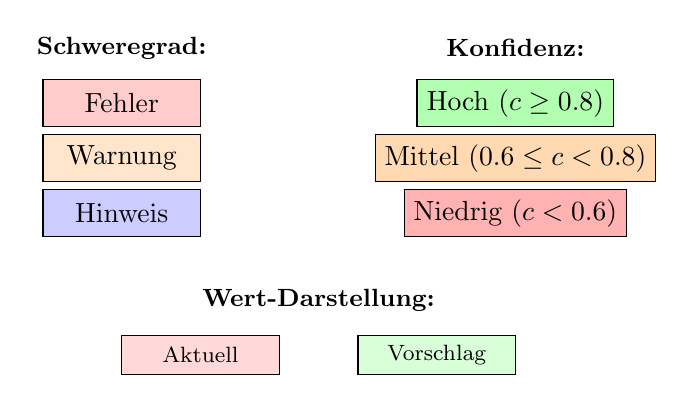
\begin{tikzpicture}

% Severity colors
\node[font=\small\bfseries] at (0,2) {Schweregrad:};
\node[rectangle, draw, fill=red!20, minimum width=2cm, minimum height=0.6cm] at (0,1.3) {Fehler};
\node[rectangle, draw, fill=orange!20, minimum width=2cm, minimum height=0.6cm] at (0,0.6) {Warnung};
\node[rectangle, draw, fill=blue!20, minimum width=2cm, minimum height=0.6cm] at (0,-0.1) {Hinweis};

% Confidence colors
\node[font=\small\bfseries] at (5,2) {Konfidenz:};
\node[rectangle, draw, fill=green!30, minimum width=2.5cm, minimum height=0.6cm] at (5,1.3) {Hoch ($c \geq 0.8$)};
\node[rectangle, draw, fill=orange!30, minimum width=2.5cm, minimum height=0.6cm] at (5,0.6) {Mittel ($0.6 \leq c < 0.8$)};
\node[rectangle, draw, fill=red!30, minimum width=2.5cm, minimum height=0.6cm] at (5,-0.1) {Niedrig ($c < 0.6$)};

% Value highlighting
\node[font=\small\bfseries] at (2.5,-1.2) {Wert-Darstellung:};
\node[rectangle, draw, fill=red!15, minimum width=2cm, minimum height=0.5cm, font=\footnotesize] at (1,-1.9) {Aktuell};
\node[rectangle, draw, fill=green!15, minimum width=2cm, minimum height=0.5cm, font=\footnotesize] at (4,-1.9) {Vorschlag};

\end{tikzpicture}
\caption{Farbkodierung für Validierungsprobleme und Korrekturvorschläge}
\label{fig:validation_color_coding}
\end{figure}


\subsubsection{Jump-to-Detection Funktionalität}

Eine wesentliche Herausforderung bei der manuellen Validierung besteht in der effizienten Lokalisierung problematischer Erkennungen im Originaldokument. Das System adressiert dies durch eine integrierte Navigation, die eine direkte Verlinkung zwischen Validierungsproblemen und der entsprechenden Position im PDF-Viewer ermöglicht.

\begin{figure}[H]
\centering
\includegraphics[width=1.0\textwidth]{images/Kapitel6/Validierungsdialog2.png} 
\caption{Jump-to-Detection Workflow zwischen Validierungsdialog und Gleisplan-Ansicht}
\label{fig:jump_to_detection}
\end{figure}

Für Validierungsprobleme, die eine räumliche Position besitzen, wird in der Tabelle eine zusätzliche Aktionsspalte mit einem Navigationsbutton bereitgestellt. Die Aktivierung dieses Buttons löst ein Signal aus, das die Identifikation der betroffenen Zeile sowie die räumlichen Koordinaten $(x, y)$ der Erkennung transportiert. Dieses Signal wird vom übergeordneten Workspace-Modul empfangen und verarbeitet. Die Verarbeitung umfasst mehrere Schritte: Zunächst wird die entsprechende Zeile im Baumansicht-Widget des Workspace selektiert, wodurch die Detailinformationen der Erkennung im unteren Panel angezeigt werden. Anschließend wird die PDF-Ansicht auf die entsprechende Seite navigiert und die Ansicht so zentriert, dass die Position der Erkennung im sichtbaren Bereich liegt. Abschließend wird ein visuelles Highlighting der Erkennungsregion aktiviert, typischerweise durch Einblendung eines farbigen Rahmens oder einer semitransparenten Überlagerung.

Die technische Implementierung dieser Funktionalität basiert auf dem Signal-Slot-Mechanismus von PyQt5. Der Validierungsdialog emittiert ein Signal, das die Zeilenidentifikation sowie die Position als Tupel überträgt. Der Workspace registriert einen Slot für dieses Signal, der die beschriebene Navigations- und Highlighting-Logik implementiert.

\subsubsection{Interaktiver Validierungsworkflow}

Der typische Arbeitsablauf bei der Validierung und Korrektur extrahierter Daten gliedert sich in mehrere Phasen. Initial wählt der Benutzer die Validierungsfunktion aus dem Anwendungsmenü, was die Ausführung aller konfigurierten Validierungsprüfungen auf dem aktuellen Datensatz initiiert. Die Validierungsengine analysiert sequenziell alle Daten und sammelt identifizierte Probleme in einer strukturierten Liste.

Nach Abschluss der Validierung wird der Ergebnisdialog präsentiert, der eine statistische Zusammenfassung der identifizierten Probleme am oberen Rand anzeigt. Diese Zusammenfassung quantifiziert die Anzahl der Fehler, Warnungen und Hinweise sowie die Anzahl automatisch korrigierbarer Probleme, aufgeschlüsselt nach Konfidenzklassen. Diese Übersicht ermöglicht eine schnelle Einschätzung des Validierungsstatus und der erforderlichen Korrekturmaßnahmen.

Der Benutzer navigiert anschließend durch die verschiedenen Tabs, um die Detailansichten der Probleme zu inspizieren. Im Tab für automatische Korrekturen werden die Korrekturvorschläge geprüft und durch Aktivierung oder Deaktivierung der zugehörigen Checkboxen selektiert. Die Anzahl der selektierten Korrekturen wird dynamisch aktualisiert und in der Beschriftung des Anwendungs-Buttons reflektiert.

Die Anwendung der selektierten Korrekturen erfolgt durch Aktivierung des entsprechenden Buttons, was zunächst einen Bestätigungsdialog aufruft. Dieser Dialog präsentiert eine Zusammenfassung der anzuwendenden Änderungen und warnt den Benutzer, dass die Modifikationen sofort im Datensatz wirksam werden. Nach Bestätigung werden die Korrekturen sequenziell auf den Datensatz angewendet, und der Dialog schließt sich. Die korrigierten Daten sind unmittelbar im Workspace sichtbar und können anschließend persistent in der Datenbank gespeichert werden.

\subsection{Persistierung und Export der Validierungsergebnisse}

\subsubsection{Export-Formate für Validierungsberichte}

Das System bietet zwei komplementäre Export-Optionen für Validierungsergebnisse, die unterschiedliche Anwendungsfälle adressieren. Der detaillierte Textbericht stellt eine menschenlesbare, narrative Darstellung der Validierungsergebnisse bereit, während der tabellarische CSV-Export eine maschinenlesbare Repräsentation für statistische Auswertungen und Weiterverarbeitung ermöglicht.

Der Textbericht beginnt mit einer strukturierten Kopfzeile, die den Berichtstyp und den Generierungszeitpunkt dokumentiert. Es folgt eine statistische Zusammenfassung, die alle aggregierten Kennzahlen der Validierung präsentiert, einschließlich der Gesamtanzahl identifizierter Probleme, der Verteilung nach Schweregraden sowie der Anzahl automatisch korrigierbarer Probleme differenziert nach Konfidenzklassen. Falls automatische Korrekturen bereits angewendet wurden, werden diese in einem separaten Abschnitt aufgelistet, wobei für jede Korrektur die Zeilenidentifikation, das betroffene Feld sowie die Transformation vom ursprünglichen zum korrigierten Wert dokumentiert wird.

Der Hauptteil des Textberichts gruppiert die identifizierten Probleme nach Kategorien. Für jede Kategorie wird ein dedizierter Abschnitt erstellt, der alle zugehörigen Probleme in strukturierter Form auflistet. Jedes Problem wird durch mehrere Zeilen beschrieben: die Zeilenidentifikation mit Schweregrad, das betroffene Feld, die detaillierte Problembeschreibung, den aktuellen fehlerhaften Wert sowie gegebenenfalls den Korrekturvorschlag inklusive Konfidenzwert. Diese narrative Struktur ermöglicht eine intuitive Erfassung der Validierungsergebnisse und eignet sich für manuelle Überprüfungen oder als Dokumentation des Validierungsprozesses.

Der tabellarische CSV-Export repräsentiert die Validierungsergebnisse in einer flachen, relationalen Struktur. Jede Zeile der CSV-Datei korrespondiert zu einem identifizierten Problem, wobei folgende Spalten definiert sind: Schweregrad als kategoriale Variable, Kategorie zur Klassifikation des Problemtyps, Zeilenidentifikation zur Referenzierung im ursprünglichen Datensatz, betroffenes Feld als Spaltenname, detaillierte Problembeschreibung als Freitext, aktueller fehlerhafter Wert, Korrekturvorschlag falls vorhanden, und Konfidenzwert des Vorschlags. Diese Struktur ermöglicht den Import in Tabellenkalkulationssoftware oder statistische Analysewerkzeuge und unterstützt quantitative Auswertungen der Validierungsergebnisse.

\subsubsection{Datenbankbasierte Persistierung}

Zur langfristigen Speicherung und Nachverfolgbarkeit werden Validierungsergebnisse in einer PostgreSQL-Datenbank persistiert. Das Datenbankschema (Abbildung~\ref{fig:validation_db_schema}) umfasst drei spezialisierte Tabellen für Validierungsprotokolle, Qualitätsmetriken und manuelle Korrekturen.

\begin{figure}[H]
\centering
\begin{tikzpicture}[
    node distance=3cm,
    table/.style={rectangle split, rectangle split parts=2, draw, minimum width=4.5cm, fill=blue!10, font=\small},
    arrow/.style={->, >=stealth, thick}
]

% Main reference table (top)
\node[table] (layout) {
    \textbf{track\_layouts}
    \nodepart{second}
    \begin{tabular}{@{}l@{}}
    \underline{id} (PK)\\
    layout\_name
    \end{tabular}
};

% validation_log table (bottom left)
\node[table, below left=2.5cm and 1cm of layout] (vlog) {
    \textbf{validation\_log}
    \nodepart{second}
    \begin{tabular}{@{}l@{}}
    \underline{id} (PK)\\
    layout\_id (FK)\\
    validation\_type\\
    severity\\
    message\\
    row\_id\\
    details (JSONB)\\
    created\_at
    \end{tabular}
};

% quality_metrics table (bottom center)
\node[table, below=2.5cm of layout] (qmetrics) {
    \textbf{quality\_metrics}
    \nodepart{second}
    \begin{tabular}{@{}l@{}}
    \underline{id} (PK)\\
    layout\_id (FK)\\
    metric\_name\\
    metric\_value\\
    metric\_data (JSONB)\\
    computed\_at
    \end{tabular}
};

% manual_corrections table (bottom right)
\node[table, below right=2.5cm and 1cm of layout] (mcorr) {
    \textbf{manual\_corrections}
    \nodepart{second}
    \begin{tabular}{@{}l@{}}
    \underline{id} (PK)\\
    layout\_id (FK)\\
    row\_id\\
    column\_name\\
    old\_value\\
    new\_value\\
    correction\_type\\
    corrected\_by\\
    correction\_reason\\
    created\_at
    \end{tabular}
};

% Foreign key relationships
\draw[arrow] (vlog.north) -- (layout.south) node[midway, left, font=\tiny, sloped] {N:1};
\draw[arrow] (qmetrics.north) -- (layout.south) node[midway, right, font=\tiny] {N:1};
\draw[arrow] (mcorr.north) -- (layout.south) node[midway, right, font=\tiny, sloped] {N:1};

% Optional: Add constraint annotations
\node[below=0.2cm of vlog.south, font=\tiny, text width=4cm, align=center] 
    {severity $\in$ \{ERROR, WARNING, INFO\}};

\end{tikzpicture}
\caption{PostgreSQL Datenbankschema für Validierungspersistierung}
\label{fig:validation_db_schema}
\end{figure}


Die Tabelle für Validierungsprotokolle (validation\_log) speichert detaillierte Informationen zu jedem identifizierten Problem. Die Struktur umfasst eine eindeutige Identifikation des Protokolleintrags, eine Referenz zum zugehörigen Gleisplan, die Klassifikation des Validierungstyps, den Schweregrad als standardisierte Kategorie (ERROR, WARNING, INFO), eine textuelle Problembeschreibung, eine optionale Referenz zur betroffenen Zeile im extrahierten Datensatz, ein JSON-Feld für zusätzliche kontextuelle Informationen sowie einen Zeitstempel der Protokollierung. Diese Struktur ermöglicht sowohl die Rekonstruktion des Validierungszustands zu einem bestimmten Zeitpunkt als auch die Analyse von Fehlertrends über mehrere Extraktionsdurchläufe hinweg.






Die Qualitätsmetriken-Tabelle (quality)aggregiert quantitative Kennzahlen zur Bewertung der Extraktionsqualität. Gespeichert werden der Name der Metrik als Identifikator, ein numerischer Wert für quantitative Metriken, ein JSON-Feld für strukturierte Metrikdaten sowie ein Zeitstempel der Berechnung. Typische Metriken umfassen die durchschnittliche YOLO-Konfidenz aggregiert über alle Klassen sowie klassenspezifisch, die OCR-Erfolgsrate für Koordinaten und Signalbezeichnungen als Quotient erfolgreich erkannter Texte zur Gesamtzahl der Objekte, die Linking-Erfolgsrate als Anteil der Objekte mit korrekt verknüpften Koordinaten, sowie die Anzahl niedrig-konfidenter Erkennungen differenziert nach Objektklasse. Diese Metriken ermöglichen eine quantitative Bewertung der Systemleistung und unterstützen die Identifikation von Optimierungspotenzialen.

Die dritte Tabelle (manual\_corrections)protokolliert manuelle Korrekturen, die durch den Benutzer nach Abschluss der automatischen Validierung vorgenommen werden. Für jede Korrektur werden die Zeilenidentifikation, der Name der modifizierten Spalte, der ursprüngliche Wert vor Korrektur, der neue Wert nach Korrektur, eine Typisierung der Korrektur zur Kategorisierung, die Identifikation des korrigierenden Benutzers, eine optionale textuelle Begründung sowie ein Zeitstempel gespeichert. Diese Daten dienen mehreren Zwecken: Sie ermöglichen eine vollständige Nachvollziehbarkeit aller Datenmodifikationen, unterstützen die Analyse häufiger Korrekturmuster zur Identifikation systematischer Fehler in der Extraktionspipeline, und liefern wertvolle Trainingsdaten für die iterative Verbesserung der zugrundeliegenden Modelle.

Zur Unterstützung statistischer Analysen wurde eine Datenbankansicht implementiert, die Korrekturstatistiken aggregiert. Diese Ansicht fasst Korrekturen nach Gleisplan und Spaltenname zusammen und berechnet die Gesamtanzahl der Korrekturen, die Anzahl betroffener unterschiedlicher Zeilen sowie den Zeitraum der ersten und letzten Korrektur. Diese aggregierten Daten ermöglichen die Identifikation besonders fehleranfälliger Datenfelder und unterstützen die Priorisierung von Verbesserungsmaßnahmen.

Die Implementierung der Datenbankpersistierung nutzt prepared statements und parametrisierte Abfragen zur Vermeidung von SQL-Injection-Vulnerabilitäten. Transaktionale Semantik gewährleistet die atomare Speicherung zusammengehöriger Datensätze. Indizes auf häufig abgefragten Spalten optimieren die Leistung bei Analyseabfragen über große Validierungsdatenmengen.

\subsection{Zusammenfassung}

Das Validierungssystem kombiniert regelbasierte Prüfungen mit intelligenten Korrekturvorschlägen und bietet eine benutzerfreundliche UI zur Qualitätssicherung. Durch Persistierung der Ergebnisse in PostgreSQL werden langfristige Qualitätsanalysen und iterative Modellverbesserungen ermöglicht. Korrekturen mit niedriger Konfidenz oder mehrdeutigen Fällen werden dem Benutzer zur manuellen Prüfung vorgelegt.

\section{Unterstützende Komponenten}
\label{sec:unterstützendekomponente}
Neben der Kernfunktionalität der Extraktionspipeline (Objekterkennung, Texterkennung, Symbol-Text-Verknüpfung) wurden mehrere unterstützende Komponenten entwickelt, die für den praktischen Einsatz des Systems in realen Anwendungsszenarien erforderlich sind. Diese Komponenten adressieren die Anforderungen an Versionsverwaltung, Rückverfolgbarkeit und persistente Datenhaltung, welche für den operativen Einsatz in ingenieurwissenschaftlichen Workflows unerlässlich sind.

\subsection{Versionsvergleich und Änderungsdetektion}
\label{subsec:vergleichundänderung}
Die systematische Identifikation und Dokumentation von Änderungen zwischen verschiedenen Versionen eines Gleisplans stellt eine zentrale Anforderung in der Eisenbahnplanung dar. Diese Funktionalität wird vom Benutzer manuell über die Benutzeroberfläche initiiert, nicht als Teil der automatischen Verarbeitungspipeline. Zur Realisierung dieser Funktionalität wurde ein Diff-Algorithmus implementiert, der auf der Generierung eindeutiger Identifikatoren und mengentheoretischen Operationen basiert.

\subsubsection{Generierung eindeutiger Identifikatoren}

Für die eindeutige Identifikation extrahierter Objekte über verschiedene Planversionen hinweg wird ein deterministischer Unique Identifier (UID) generiert. Die UID-Generierung erfolgt durch Konkatenation der Objektklasse, des normalisierten Textinhalts und eines räumlichen Index, um Dopplungen bei identischem Textinhalt zu vermeiden:

\begin{equation} \text{UID}(o) = \text{class}(o) \oplus \text{normalize}(\text{content}(o)) \oplus \text{GridIndex}(x, y) \end{equation}

wobei GridIndex(x,y) die Koordinaten auf ein grobes Raster abbildet, um Robustheit gegen minimale Pixelverschiebungen zu gewährleisten, während Identität bei gleicher Semantik an verschiedenen Orten unterschieden wird. $\oplus$ bezeichnet die String-Konkatenation und die Normalisierungsfunktion $\text{normalize}: \Sigma^* \rightarrow \Sigma^*$ Leerzeichen entfernt und Sonderzeichen standardisiert, um konsistente Identifikatoren zu gewährleisten.
\begin{figure}[H]
\centering
\begin{tikzpicture}[
    node distance=1.5cm,
    box/.style={rectangle, draw, minimum width=2.5cm, minimum height=0.8cm, align=center},
    arrow/.style={->, >=stealth, thick}
]

% Example 1: Signal
\node[box] (sig1) {Signal\\AS102};
\node[box, below=0.5cm of sig1] (sig2) {class: ``signal''\\text: ``AS102''};
\node[box, below=0.5cm of sig2] (sig3) {\texttt{signal\_AS102}};

\draw[arrow] (sig1) -- (sig2) node[midway, right, font=\small] {Extraktion};
\draw[arrow] (sig2) -- (sig3) node[midway, right, font=\small] {UID-Gen.};

% Example 2: GKS
\node[box, right=2cm of sig1] (gks1) {GKS\\12345};
\node[box, below=0.5cm of gks1] (gks2) {class: ``gks''\\text: ``12345''};
\node[box, below=0.5cm of gks2] (gks3) {\texttt{gks\_12345}};

\draw[arrow] (gks1) -- (gks2);
\draw[arrow] (gks2) -- (gks3);

% Example 3: Coordinate
\node[box, right=2cm of gks1] (coord1) {Koordinate\\18.1606};
\node[box, below=0.5cm of coord1] (coord2) {class: ``coordinate''\\text: ``18.1606''};
\node[box, below=0.5cm of coord2] (coord3) {\texttt{coordinate\_18.1606}};

\draw[arrow] (coord1) -- (coord2);
\draw[arrow] (coord2) -- (coord3);

\end{tikzpicture}
\caption{Schematische Darstellung des UID-Generierungsprozesses für verschiedene Objekttypen}
\label{fig:uid_generation}
\end{figure}


\textbf{Beispiele für generierte UIDs:}
\begin{itemize}
    \item Signal mit Bezeichnung ``AS102'' $\rightarrow$ \texttt{signal\_AS102}
    \item GKS mit Kennung ``12345'' $\rightarrow$ \texttt{gks\_12345}
    \item Kilometerangabe ``18.1606'' $\rightarrow$ \texttt{coordinate\_18.1606}
\end{itemize}

Die Verwendung von UIDs ermöglicht eine effiziente Objektzuordnung zwischen Planversionen, selbst bei Änderungen der räumlichen Position oder anderer Attribute.

\subsubsection{Differenzalgorithmus}

Der Vergleichsalgorithmus basiert auf mengentheoretischen Operationen zwischen zwei Extraktionsmengen $A$ (Altversion) und $B$ (Neuversion). Seien $A = \{a_1, a_2, \ldots, a_m\}$ und $B = \{b_1, b_2, \ldots, b_n\}$ die Mengen extrahierter Objekte mit ihren UIDs als Mengenelemente.


\textbf{Primäre Differenzmengen:}
\begin{align}
\Delta_{\text{add}} &= B \setminus A \quad \text{(hinzugefügte Objekte)} \\
\Delta_{\text{rem}} &= A \setminus B \quad \text{(entfernte Objekte)} \\
\Delta_{\text{pot}} &= A \cap B \quad \text{(potentiell modifizierte Objekte)}
\end{align}

\begin{figure}[H]
\centering
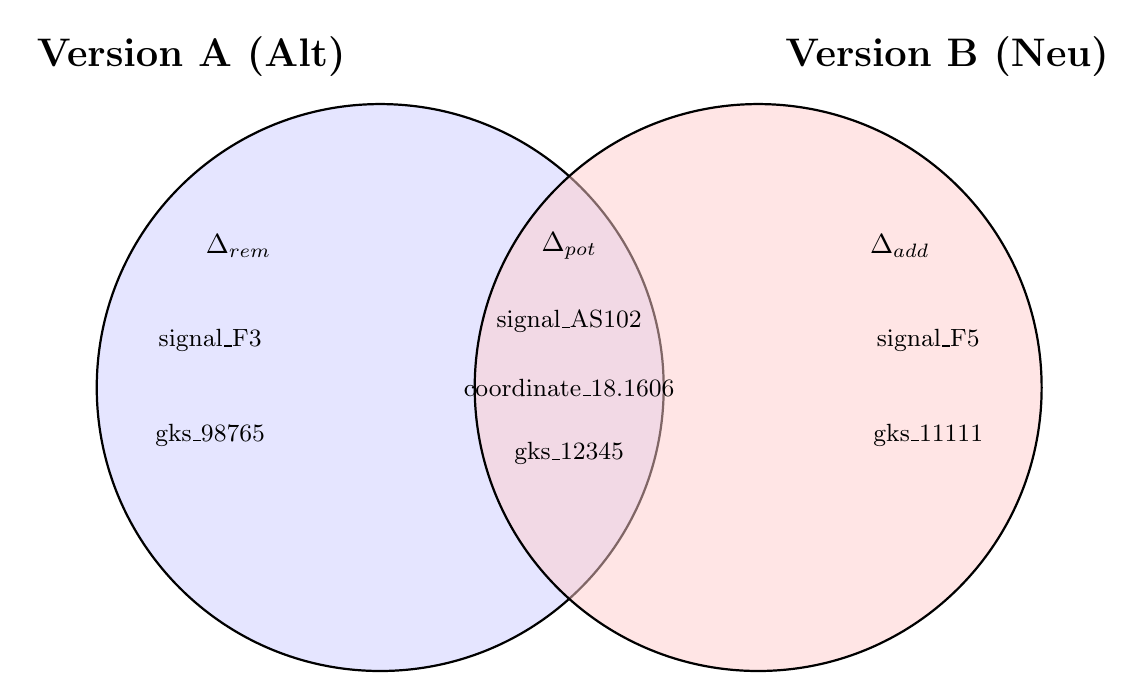
\begin{tikzpicture}[scale=1.2]
    % Draw two bigger circles, adjust position of the second circle
    \draw[thick, fill=blue!20, fill opacity=0.5] (0,0) circle (3cm);
    \draw[thick, fill=red!20, fill opacity=0.5] (4,0) circle (3cm);

    % Labels for circles, adjusted position
    \node at (-2, 3.5) {\Large\textbf{Version A (Alt)}};
    \node at (6, 3.5) {\Large\textbf{Version B (Neu)}};

    % Region labels, adjusted position (moved up)
    \node at (-1.5, 1.5) {\textbf{$\Delta_{\text{rem}}$}};
    \node at (2, 1.5) {\textbf{$\Delta_{\text{pot}}$}};
    \node at (5.5, 1.5) {\textbf{$\Delta_{\text{add}}$}};

    % Example objects, adjusted positions to fit the larger circles
    \node[font=\small] at (-1.8, 0.5) {signal\_F3};
    \node[font=\small] at (-1.8, -0.5) {gks\_98765};

    \node[font=\small] at (2, 0.7) {signal\_AS102};
    \node[font=\small] at (2, 0) {coordinate\_18.1606};
    \node[font=\small] at (2, -0.7) {gks\_12345};
    \node[font=\small] at (5.8, 0.5) {signal\_F5};
    \node[font=\small] at (5.8, -0.5) {gks\_11111};

    % Legend removed as requested
\end{tikzpicture}
\caption{Mengentheoretische Visualisierung des Diff-Algorithmus}
\label{fig:diff_algorithm}
\end{figure}
Für Objekte in der Schnittmenge $\Delta_{\text{pot}}$ wird eine attributbasierte Änderungsanalyse durchgeführt. Sei $o_A \in A$ und $o_B \in B$ ein korrespondierendes Objektpaar mit identischer UID, dann erfolgt der Vergleich folgender Attribute:

\textbf{Textmodifikation:}
\begin{equation}
\text{isModified}_{\text{text}}(o_A, o_B) = \begin{cases}
\text{true}, & \text{falls } \text{content}(o_A) \neq \text{content}(o_B) \\
\text{false}, & \text{sonst}
\end{cases}
\end{equation}

\textbf{Positionsänderung:}
Zur Detektion signifikanter Positionsänderungen wird die euklidische Distanz zwischen den Zentroiden berechnet:

\begin{equation}
d(o_A, o_B) = \sqrt{(x_B - x_A)^2 + (y_B - y_A)^2}
\end{equation}

wobei $(x_A, y_A)$ und $(x_B, y_B)$ die Koordinaten der jeweiligen Objektzentroiden in Pixeln bezeichnen. Ein Objekt gilt als räumlich verschoben, falls:

\begin{equation}
\text{isMoved}(o_A, o_B) = \begin{cases}
\text{true}, & \text{falls } d(o_A, o_B) > \tau_{\text{dist}} \\
\text{false}, & \text{sonst}
\end{cases}
\end{equation}


\begin{figure}[H]
\centering
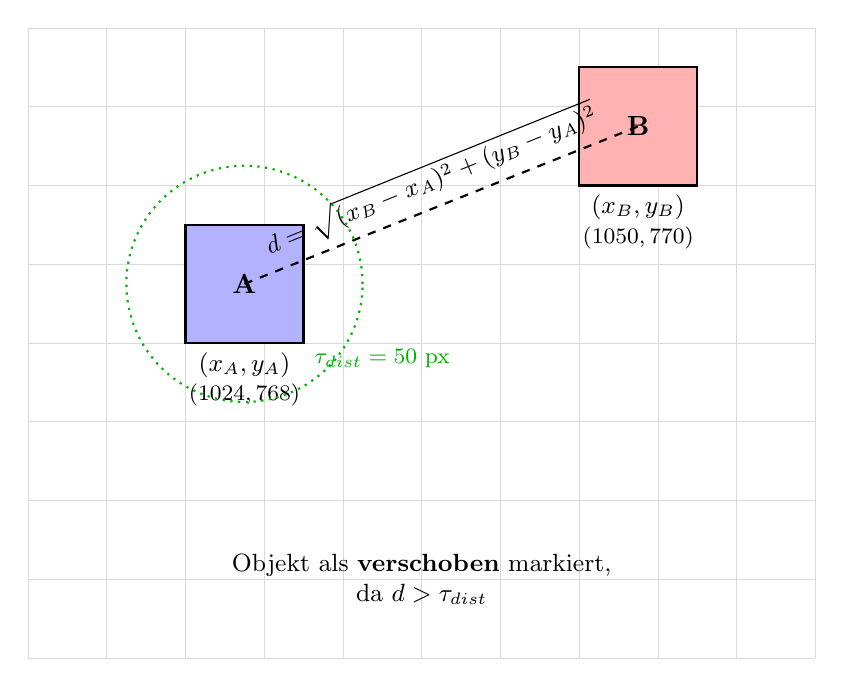
\begin{tikzpicture}[scale=1.0]
    % Grid
    \draw[step=1cm, gray!30, very thin] (0,0) grid (10,8);
    
    % Object in Version A (old position)
    \draw[thick, fill=blue!30] (2,4) rectangle (3.5,5.5);
    \node at (2.75, 4.75) {\textbf{A}};
    \node[below, font=\small] at (2.75, 4) {$(x_A, y_A)$};
    \node[below, font=\footnotesize] at (2.75, 3.6) {$(1024, 768)$};
    
    % Object in Version B (new position)
    \draw[thick, fill=red!30] (7,6) rectangle (8.5,7.5);
    \node at (7.75, 6.75) {\textbf{B}};
    \node[below, font=\small] at (7.75, 6) {$(x_B, y_B)$};
    \node[below, font=\footnotesize] at (7.75, 5.6) {$(1050, 770)$};
    
    % Distance line
    \draw[thick, dashed, color=black] (2.75, 4.75) -- (7.75, 6.75);
    \node[above, rotate=22, color=black, font=\small] at (5.25, 5.75) {$d = \sqrt{(x_B-x_A)^2 + (y_B-y_A)^2}$};
    
    % Threshold circle (schematic)
    \draw[dotted, thick, color=green!70!black] (2.75, 4.75) circle (1.5cm);
    \node[font=\footnotesize, color=green!70!black] at (4.5, 3.8) {$\tau_{\text{dist}} = 50$ px};
    
    % Annotation
    \node[align=center, font=\small] at (5, 1) {
        Objekt als \textbf{verschoben} markiert,\\
        da $d > \tau_{\text{dist}}$
    };
\end{tikzpicture}
\caption{Geometrische Darstellung der Positionsänderungserkennung mit euklidischer Distanz}
\label{fig:position_change}
\end{figure}

Der empirisch ermittelte Schwellenwert $\tau_{\text{dist}} = 50$ Pixel berücksichtigt geringfügige Positionsschwankungen durch PDF-Rendering-Variationen und fokussiert auf semantisch relevante Verschiebungen.

\subsubsection{Strukturierte Änderungsdokumentation}

Die identifizierten Änderungen werden in einem strukturierten Change Report dokumentiert, der als Excel-Datei exportiert wird und folgende Informationen je Änderung enthält:

\begin{table}[H]
\centering
\small
\begin{tabular}{|l|l|p{3.5cm}|p{3.5cm}|}
\hline
\textbf{UID} & \textbf{Änderungstyp} & \textbf{Zustand (Alt)} & \textbf{Zustand (Neu)} \\
\hline
signal\_AS102 & Verschoben & $x=1024, y=768$ & $x=1050, y=770$ \\
signal\_F5 & Hinzugefügt & $-$ & $x=2300, y=1200$ \\
gks\_98765 & Entfernt & $x=1500, y=900$ & $-$ \\
coordinate\_18.1606 & Textänderung & Text: ``18.1606'' & Text: ``18.1608'' \\
\hline
\end{tabular}
\caption{Beispielhafte Change Report Struktur mit verschiedenen Änderungstypen}
\label{tab:change_report}
\end{table}

Diese strukturierte Dokumentation ermöglicht eine effiziente Nachvollziehbarkeit von Planänderungen und unterstützt Quality-Assurance-Prozesse in der Eisenbahnplanung.
Die Implementierung umfasst eine dedizierte grafische Benutzeroberfläche zur Visualisierung und Analyse der Änderungen, wie in Abbildung~\ref{fig:diff_ui} dargestellt.

\begin{figure}[H]
\centering
\includegraphics[width=0.98\textwidth]{images/Kapitel6/diff_dialog.png}
\caption{Versionsvergleichs-Dialog mit tabellarischer Auflistung aller Änderungen zwischen zwei Planversionen}
\label{fig:diff_ui}
\end{figure}

Der Dialog zeigt eine tabellarische Übersicht aller identifizierten Änderungen mit Spalten für Objektklasse, Text, Feldname, alte und neue Werte sowie Seitenzuordnung. In diesem Beispiel wurden fünf GKS-Koordinaten modifiziert, wobei die Verschiebungen im Bereich von +0{,}0m bis +0{,}6m liegen. Die Änderungstypen werden durch Icons visualisiert: Hinzugefügte Elemente erhalten ein grünes Plus-Symbol, entfernte Elemente ein rotes Minus-Symbol, und modifizierte Werte werden orange hervorgehoben. Diese Darstellung erfüllt Anforderung FA-011 und ermöglicht Ingenieuren eine schnelle Identifikation relevanter Planänderungen ohne manuelle Vergleichsarbeit.

Ein konkretes Beispiel einer detektierten Koordinatenänderung zeigen die Abbildungen~\ref{fig:gks_change_before} und~\ref{fig:gks_change_after} für die GKS-Platte mit der Kennung 0305.

\begin{figure}[H]
\centering
\begin{minipage}{0.48\textwidth}
    \centering
    \includegraphics[width=0.8\textwidth]{images/Kapitel6/gkschange1.png}
    \caption{GKS 0305 in Version 1: Koordinate 0.1770}
    \label{fig:gks_change_before}
\end{minipage}
\hfill
\begin{minipage}{0.48\textwidth}
    \centering
    \includegraphics[width=\textwidth]{images/Kapitel6/gkschange2.png}
    \caption{GKS 0305 in Version 2: Koordinate 0.1729}
    \label{fig:gks_change_after}
\end{minipage}
\end{figure}

Die automatische Änderungsdetektion identifizierte eine Verschiebung um $\Delta = -0{,}0041$ km (ca. 4,1 Meter) durch UID-basierten Objektvergleich. Der Algorithmus erkannte, dass beide Versionen dasselbe Objekt (\texttt{gks\_gesteuert\_0305}) beschreiben, jedoch unterschiedliche Koordinatenwerte aufweisen. Solche Präzisionsänderungen im Meterbereich sind in der Feinplanung von Bahnanlagen kritisch und müssen dokumentiert werden, da sie die Positionierung sicherheitsrelevanter Komponenten betreffen.
\subsection{Rückverfolgbarkeit zur Quelldokumentation}

Die vollständige Rückverfolgbarkeit extrahierter Daten zur Originalquelle ist essentiell für die Validierung und manuelle Nachkorrektur von Extraktionsergebnissen. Hierzu wird für jeden extrahierten Datensatz ein umfassender Metadatensatz persistiert.
\begin{figure}[H]
\centering
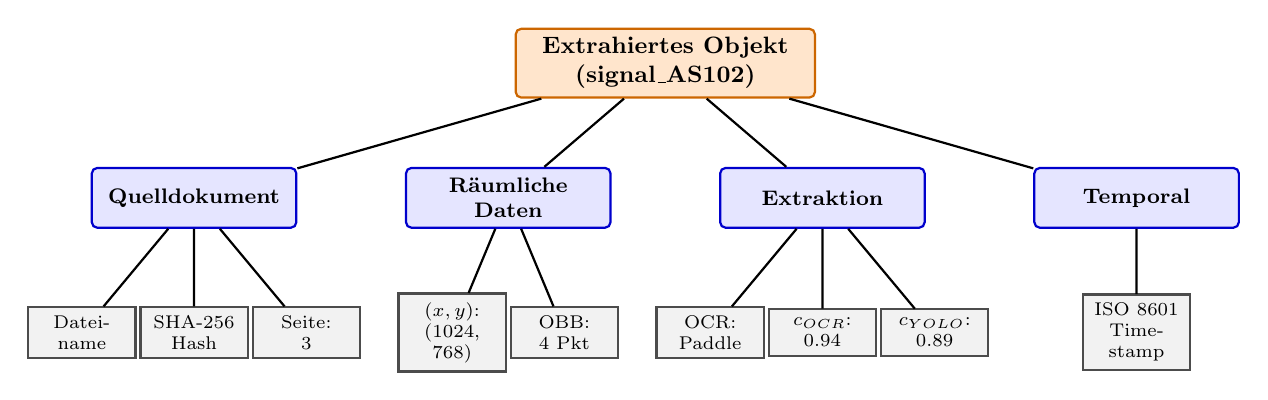
\begin{tikzpicture}[
    scale=0.95, 
    transform shape,
    % --- Baum-Einstellungen ---
    level 1/.style={sibling distance=4.2cm, level distance=1.8cm}, % Weiter auseinander für Platz
    level 2/.style={sibling distance=1.5cm, level distance=1.8cm}, % Enger zusammen
    edge from parent/.style={draw, thick, black},
    % --- Styles ---
    box/.style={
        rectangle, 
        draw=blue!80!black, 
        thick,
        rounded corners=2pt, 
        fill=blue!10, 
        minimum width=2.5cm, 
        text width=2.5cm, % Erzwingt Umbruch
        minimum height=0.8cm, 
        align=center, 
        font=\footnotesize\bfseries
    },
    subbox/.style={
        rectangle, 
        draw=gray!60!black, 
        fill=gray!10, 
        minimum width=1.2cm, 
        text width=1.2cm, % Schmale Spalten für Blätter
        minimum height=0.6cm, 
        align=center, 
        font=\scriptsize
    },
    rootbox/.style={
        rectangle,
        draw=orange!80!black,
        thick,
        rounded corners=2pt,
        fill=orange!20,
        minimum width=4cm,
        align=center,
        font=\small\bfseries
    }
]

% Root
\node[rootbox] {Extrahiertes Objekt\\(signal\_AS102)}
    % Branch 1: Quelldokument
    child {node[box] {Quelldokument}
        child {node[subbox] {Datei-\\name}}
        child {node[subbox] {SHA-256\\Hash}}
        child {node[subbox] {Seite:\\3}}
    }
    % Branch 2: Räumliche Daten
    child {node[box] {Räumliche\\Daten}
        child {node[subbox] {$(x, y)$:\\(1024,\\768)}}
        child {node[subbox] {OBB:\\4 Pkt}}
    }
    % Branch 3: Extraktion
    child {node[box] {Extraktion}
        child {node[subbox] {OCR:\\Paddle}}
        child {node[subbox] {$c_{\text{OCR}}$:\\0.94}}
        child {node[subbox] {$c_{\text{YOLO}}$:\\0.89}}
    }
    % Branch 4: Temporal
    child {node[box] {Temporal}
        child {node[subbox] {ISO 8601\\Time-\\stamp}}
    };

\end{tikzpicture}
\caption{Hierarchische Struktur der Metadaten für ein extrahiertes Objekt}
\label{fig:metadata_structure}
\end{figure}

\subsubsection{Metadatenmodell}

Das Metadatenmodell umfasst folgende Informationsebenen:

\textbf{Quelldokument-Identifikation:}
\begin{itemize}
    \item Dateiname der Quell-PDF ($f_{\text{source}}$)
    \item Kryptographischer Hash (SHA-256) zur Integritätssicherung
    \item Seitennummer innerhalb des Dokuments ($p \in \mathbb{N}$)
\end{itemize}

\textbf{Räumliche Lokalisierung:}
\begin{itemize}
    \item Zentroid-Koordinaten in absoluten Pixelkoordinaten: $(x, y) \in \mathbb{R}^2$
    \item Oriented Bounding Box Geometrie: $\text{OBB} = \{(x_1, y_1), (x_2, y_2), (x_3, y_3), (x_4, y_4)\}$
    \item Die OBB-Repräsentation ermöglicht die präzise Visualisierung rotierter Textelemente
\end{itemize}

\textbf{Extraktionsdetails:}
\begin{itemize}
    \item Verwendete OCR-Engine ($e \in \{\text{PaddleOCR}, \text{Tesseract}, \text{EasyOCR}\}$)
    \item Konfidenzscore der Objekterkennung: $c_{\text{YOLO}} \in [0, 1]$
    \item Konfidenzscore der Texterkennung: $c_{\text{OCR}} \in [0, 1]$
    \item Angewandte Linking-Methode ($m \in \{\text{standard}, \text{adaptive}\}$)
\end{itemize}

\textbf{Temporale Zuordnung:}
\begin{itemize}
    \item ISO 8601 formatierter Zeitstempel der Extraktion
\end{itemize}

\subsubsection{Integration in die Benutzeroberfläche}

Die Metadaten werden zur Realisierung einer bidirektionalen Navigation zwischen Datenansicht und Quelldokument genutzt:

\textbf{Tabellenbasierte Navigation:}
Beim Anklicken eines Datensatzes in der Ergebnistabelle wird der PDF-Viewer auf die entsprechende Seite navigiert, auf die dokumentierten Koordinaten zentriert und das Objekt mittels farbkodiertem Overlay hervorgehoben. Die OBB-Geometrie ermöglicht dabei eine pixelgenaue Umrandung auch bei rotierten Textelementen.

\textbf{PDF-basierte Navigation:}
Interaktives Anklicken eines visualisierten Objekts im PDF-Viewer triggert ein automatisches Scrolling zur korrespondierenden Zeile in der Ergebnistabelle, wodurch die zugehörigen Extraktionsdaten unmittelbar einsehbar werden.

Diese Funktionalität reduziert den kognitiven Aufwand bei der manuellen Validierung signifikant und ermöglicht eine effiziente Identifikation systematischer Extraktionsfehler.




\subsection{Persistente Datenhaltung}

Das System verwendet PostgreSQL (Version 14.9) zur persistenten Speicherung von Extraktionsergebnissen, Workspace-Zuständen und Qualitätsmetriken.
\begin{figure}[H]
\centering
\includegraphics[width=0.9\textwidth]{images/Kapitel6/Postgresql datenbank diagramm .png} 
\caption{Datenbankschema mit Kardinalitäten (vereinfachte Darstellung)}
\label{fig:database_schema}
\end{figure}

\subsubsection{Datenbankschema}

Das Datenbankschema ist auf die Anforderungen eines dokumentbasierten Workflows optimiert und nutzt JSONB-Datentypen für flexible Speicherung semi-strukturierter Extraktionsdaten:

\begin{verbatim}
Relation: track_layouts
-----------------------
id                SERIAL PRIMARY KEY
layout_name       TEXT UNIQUE NOT NULL

Relation: workspaces
--------------------
id                SERIAL PRIMARY KEY
layout_id         INTEGER UNIQUE NOT NULL REFERENCES track_layouts(id) 
                  ON DELETE CASCADE
edited_data_json  JSONB NOT NULL              -- Extraktionsergebnisse
track_skeleton    TEXT                        -- Komprimiertes Gleisskelett
image_dimensions  JSONB                       -- Seitenabmessungen
last_modified     TIMESTAMPTZ DEFAULT NOW()

Relation: validation_log
------------------------
id                SERIAL PRIMARY KEY
layout_id         INTEGER NOT NULL REFERENCES track_layouts(id)
validation_type   VARCHAR(100) NOT NULL
severity          VARCHAR(20) CHECK (severity IN ('ERROR', 'WARNING', 'INFO'))
message           TEXT NOT NULL
row_id            INTEGER                     -- Referenz zu Datensatz
details           JSONB
created_at        TIMESTAMPTZ DEFAULT NOW()

Relation: quality_metrics
-------------------------
id                SERIAL PRIMARY KEY
layout_id         INTEGER NOT NULL REFERENCES track_layouts(id)
metric_name       VARCHAR(100) NOT NULL
metric_value      REAL
metric_data       JSONB
computed_at       TIMESTAMPTZ DEFAULT NOW()

Relation: manual_corrections
----------------------------
id                SERIAL PRIMARY KEY
layout_id         INTEGER NOT NULL REFERENCES track_layouts(id)
row_id            INTEGER NOT NULL
column_name       VARCHAR(100) NOT NULL
old_value         TEXT
new_value         TEXT
correction_type   VARCHAR(50)
corrected_by      VARCHAR(100) DEFAULT 'user'
correction_reason TEXT
created_at        TIMESTAMPTZ DEFAULT NOW()

-- Performance-Indizes
CREATE INDEX idx_validation_log_layout ON validation_log(layout_id);
CREATE INDEX idx_validation_log_severity ON validation_log(severity);
CREATE INDEX idx_quality_metrics_layout ON quality_metrics(layout_id);
CREATE INDEX idx_manual_corrections_layout ON manual_corrections(layout_id);
\end{verbatim}

\subsubsection{JSONB-basierte Datenspeicherung}

Die Extraktionsergebnisse werden als JSONB-Array in \texttt{edited\_data\_json} gespeichert. Diese Designentscheidung bietet mehrere Vorteile gegenüber einer vollständig normalisierten Tabellenstruktur:

\textbf{Datenstruktur:}
Jeder Eintrag in \texttt{edited\_data\_json} repräsentiert ein extrahiertes Objekt mit folgender Struktur:

\begin{verbatim}
{
  "row_id": 42,
  "cls": "signal",
  "anchor_text": "AS102",
  "coord_text": "18.1606(GL2)",
  "coord_value": 18.1606,
  "x": 1024.5,
  "y": 768.3,
  "obb_points": [[x1,y1], [x2,y2], [x3,y3], [x4,y4]],
  "conf": 0.94,
  "fahrtrichtung": "A",
  ...
}
\end{verbatim}

\textbf{Vorteile des JSONB-Ansatzes:}
\begin{itemize}
    \item \textbf{Schema-Flexibilität:} Neue Attribute können ohne Datenbankmigrationen hinzugefügt werden
    \item \textbf{Atomare Updates:} Gesamter Workspace wird als Einheit gespeichert, konsistent mit UI-Operationen
    \item \textbf{Effiziente Queries:} PostgreSQL JSONB unterstützt Indexierung und performante Abfragen
    \item \textbf{Versionierung:} Einfaches Speichern vollständiger Snapshots zu verschiedenen Zeitpunkten
\end{itemize}



\subsubsection{Verwendungszwecke}

Die Datenbank erfüllt folgende funktionale Anforderungen im operativen Workflow:

\begin{itemize}
    \item \textbf{Session-Persistierung:} Speicherung von Workspace-Zuständen ermöglicht Unterbrechung und spätere Fortsetzung der Arbeit
    
    \item \textbf{Validierungs-Tracking:} Die Tabelle \texttt{validation\_log} dokumentiert alle identifizierten Datenqualitätsprobleme mit Schweregradklassifikation (ERROR, WARNING, INFO), was eine systematische Fehleranalyse ermöglicht
    
    \item \textbf{Korrektur-Historisierung:} Manuelle Benutzerkorrekturen werden in \texttt{manual\_corrections} protokolliert. Diese Daten können zur Identifikation systematischer Extraktionsfehler und zur Verbesserung der Pipeline genutzt werden
    
    \item \textbf{Qualitätsmetriken:} Aggregierte Qualitätskennzahlen (z.B. durchschnittliche OCR-Konfidenz, Vollständigkeitsraten) werden in \texttt{quality\_metrics} persistiert für longitudinale Analysen
    
    \item \textbf{Export-Vorbereitung:} Vor dem Excel-Export werden Daten aus der Datenbank geladen, validiert und transformiert
\end{itemize}

\subsubsection{Datenbankzugriff}

Die Datenbankinteraktion erfolgt über den PostgreSQL-Adapter \texttt{psycopg2} (Version 2.9.7). Die Datenbankoperationen sind in einem dedizierten Modul \texttt{database.py} gekapselt, welches folgende Kern-API bereitstellt:

\textbf{Workspace-Operationen:}
\begin{itemize}
    \item $\texttt{save\_workspace\_data}(name, data, skeleton, dims) \rightarrow \text{void}$ \\
    Persistiert Workspace mit Extraktionsdaten, optionalem Gleisskelett und Bildabmessungen
    
    \item $\texttt{get\_workspace\_data}(name) \rightarrow (data, skeleton, dims)$ \\
    Lädt gespeicherten Workspace inkl. Dekompression des Gleisskeletts
\end{itemize}

\textbf{Validierungs-Operationen:}
\begin{itemize}
    \item $\texttt{save\_validation\_results}(name, results) \rightarrow \text{void}$ \\
    Speichert Validierungsergebnisse mit automatischer Historisierung
    
    \item $\texttt{get\_validation\_summary}(name) \rightarrow \text{dict}$ \\
    Liefert Zusammenfassung nach Schweregrad aggregiert
\end{itemize}

\textbf{Korrektur-Operationen:}
\begin{itemize}
    \item $\texttt{log\_manual\_correction}(name, row, field, old, new) \rightarrow \text{void}$ \\
    Protokolliert Benutzerkorrektur für spätere Analyse
    
    \item $\texttt{get\_correction\_statistics}(name) \rightarrow \text{list}$ \\
    Analysiert Korrekturmuster zur Identifikation systematischer Fehler
\end{itemize}

Die Verwendung von Connection-Pooling mittels Context Manager optimiert die Performance bei häufigen Datenbankzugriffen während des Extraktionsprozesses und stellt automatisches Rollback bei Fehlern sicher.

\section{Benutzeroberfläche}
\label{sec:benutzeroberfläche}
Die Benutzeroberfläche dient als interaktive Komponente zur Qualitätskontrolle und 
manuellen Nachbearbeitung der extrahierten Daten. Sie adressiert die Anforderungen 
\textbf{FA-013} (GUI ohne CLI-Kenntnisse), \textbf{FA-012} (visuelle Validierung 
durch Bounding-Box-Overlays) und \textbf{NFA-001} (On-Premise-Verarbeitung als 
Desktop-Anwendung).

% === NEW SUBSECTION TO ADD ===
\subsection{Setup- und Analysedialog}
\label{subsec:setup_dialog}

Der initiale Einstiegspunkt der Anwendung \enquote{RailDoc Studio} ist der 
Setup- und Analysedialog (Abbildung~\ref{fig:setup_analyse_dialog}), der einen 
geführten dreistufigen Workflow zur Initiierung der Datenextraktion implementiert. 

\begin{figure}[H]
\centering
\includegraphics[width=0.95\textwidth]{images/Kapitel6/setup_analyse_dialog.png}
\caption{Setup- und Analyse-Dialog der Anwendung \enquote{RailDoc Studio}}
\label{fig:setup_analyse_dialog}
\end{figure}

Der Workflow gliedert sich in drei sequenzielle Schritte:

\begin{enumerate}
    \item \textbf{Gleisplan laden:} Auswahl der zu verarbeitenden PDF-Datei 
    über einen Dateidialog. Das System akzeptiert PDF-Dateien beliebiger Größe 
    und zeigt einen Hinweis zur empfohlenen Mindestauflösung von 300~DPI an, 
    wobei 500~DPI für optimale Erkennungsleistung empfohlen werden 
    (vgl. Anforderung \textbf{NFA-010}).
    
    \item \textbf{KI-Modell laden:} Auswahl der trainierten YOLOv8-OBB 
    Gewichtsdatei (\texttt{best.pt}). Diese explizite Trennung von Anwendung 
    und Modell erfüllt Anforderung \textbf{NFA-009} (Update-Fähigkeit) und 
    ermöglicht den Austausch von Modellversionen -- beispielsweise nach einem 
    Nachtraining mit zusätzlichen Symbolklassen -- ohne Neukompilierung der 
    Anwendung.
    
    \item \textbf{Analyse starten:} Initiierung der automatischen 
    Verarbeitungspipeline durch Betätigung der Schaltfläche 
    \enquote{Analyse starten}. Der Fortschrittsbalken visualisiert die drei 
    Pipeline-Stufen: Symbol-Erkennung (YOLO), Texterkennung (OCR) und 
    Gleiserkennung (Linking).
\end{enumerate}

Die Checkbox \enquote{Vollständige Neuanalyse} ermöglicht das Überschreiben 
bereits in der PostgreSQL-Datenbank gespeicherter Ergebnisse, was für 
iterative Verbesserungen oder nach Modell-Updates relevant ist. Die 
Schaltfläche \enquote{Neues Symbol definieren} (rechts oben) öffnet einen 
Assistenten zur Definition zusätzlicher Symbolklassen und demonstriert die 
Erweiterbarkeit des Systems gemäß Anforderung \textbf{NFA-008}.

Nach Abschluss der automatischen Analyse wechselt die Anwendung automatisch 
in den Bearbeitungs- und Korrekturmodus (Abschnitt~\ref{subsec:interaktiveergebnistabelle}), 
in dem die extrahierten Daten validiert und bei Bedarf manuell korrigiert 
werden können.

% === END OF NEW SUBSECTION ===

\subsection{Architektur und Designentscheidungen}

Die Architektur der Benutzeroberfläche basiert auf dem Model-View-Controller (MVC) Entwurfsmuster, wobei die Datenhaltung (Model), die Visualisierung (View) und die Ereignisverarbeitung (Controller) klar voneinander getrennt sind. Diese Architektur gewährleistet Wartbarkeit und ermöglicht die unabhängige Weiterentwicklung der einzelnen Schichten.

Die Hauptkomponenten gliedern sich in:
\begin{itemize}
    \item \textbf{Hauptfenster}: Verwaltung mehrerer parallel geöffneter PDF-Dokumente in Tab-Ansicht
    \item \textbf{Arbeitsbereich}: Dedizierter Anzeigebereich für ein einzelnes PDF-Dokument mit allen zugehörigen Extraktionsergebnissen
    \item \textbf{Interaktive PDF-Ansicht}: Visualisierung des Originaldokuments mit überlagerten Erkennungsergebnissen
    \item \textbf{Hierarchische Ergebnistabelle}: Strukturierte Darstellung aller extrahierten Daten mit Excel-ähnlicher Editierfunktionalität
    \item \textbf{Validierungs-Dialog}: Spezialisierte Komponente zur systematischen Fehlerprüfung und -korrektur
    \item \textbf{Versionsvergleichs-Modul}: Werkzeug zur Gegenüberstellung verschiedener Planversionen
\end{itemize}

Die technologische Basis bildet ein cross-platform GUI-Framework mit nativer Desktop-Integration, leistungsfähigen PDF-Rendering-Fähigkeiten sowie einer umfangreichen Widget-Bibliothek für komplexe Benutzerinteraktionen.

\subsection{PDF-Viewer mit Overlay-System}

\subsubsection{Rendering-Pipeline}

Das PDF-Rendering erfolgt in zwei Schritten: Zunächst wird jede PDF-Seite bei hoher Auflösung (500 DPI) in ein Raster-Bild konvertiert. Die Anzeigebreite $w_{\text{display}}$ berechnet sich aus der Seitenbreite $w_{\text{page}}$, der Auflösung $r$ und dem Zoomfaktor $z$ gemäß:

\begin{equation}
w_{\text{display}} = w_{\text{page}} \times \frac{r}{72} \times z
\end{equation}

wobei 72 die Standard-DPI-Referenz für PDF-Dokumente darstellt. Der Zoomfaktor $z$ ist im Bereich $[0.25, 4.0]$ steuerbar, was eine 16-fache Vergrößerungsspanne ermöglicht. Zur Performance-Optimierung wird ein Viewport-basiertes Culling implementiert (Abbildung~\ref{fig:viewport_culling}), das die Anzahl zu rendernder Overlays auf die im aktuellen Sichtbereich befindlichen Objekte reduziert. Dies verbessert die Darstellungsgeschwindigkeit bei großformatigen Plänen erheblich.
\begin{figure}[H]
\centering
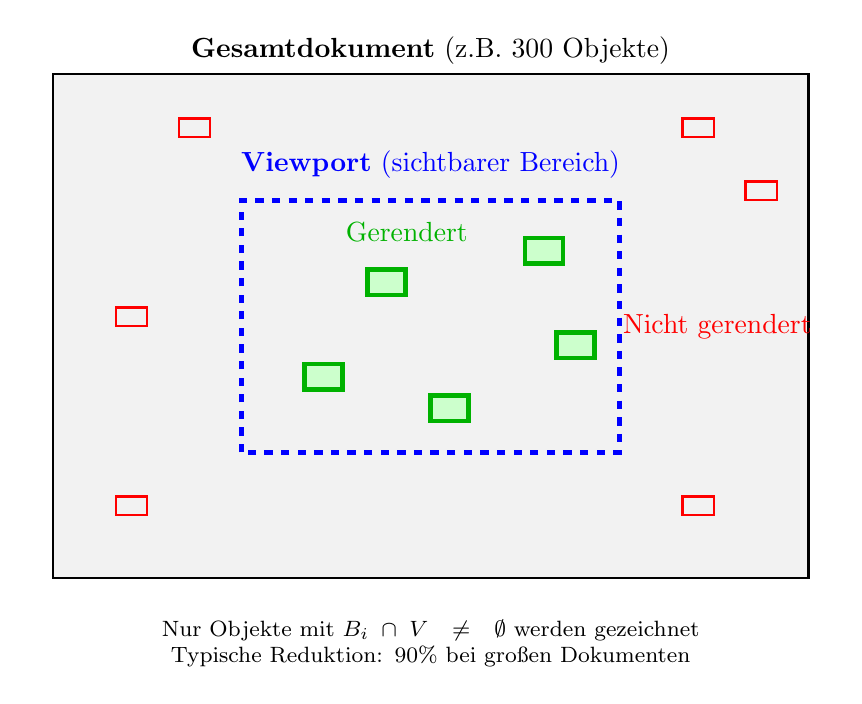
\begin{tikzpicture}[scale=0.8]

% Full document (gray background)
\fill[gray!10] (0,0) rectangle (12,8);
\draw[thick] (0,0) rectangle (12,8);
\node[above] at (6,8) {\textbf{Gesamtdokument} (z.B. 300 Objekte)};

% Viewport (blue outline)
\draw[blue, ultra thick, dashed] (3,2) rectangle (9,6);
\node[blue, above] at (6,6.2) {\textbf{Viewport} (sichtbarer Bereich)};

% Objects outside viewport (red, small)
\foreach \x/\y in {1/1, 2/7, 10/1, 11/6, 1/4, 10/7} {
    \draw[red, thick] (\x,\y) rectangle ++(0.5,0.3);
}
\node[red, right] at (8.9,4) {Nicht gerendert};

% Objects inside viewport (green, highlighted)
\foreach \x/\y in {4/3, 5/4.5, 6/2.5, 7.5/5, 8/3.5} {
    \draw[green!70!black, ultra thick, fill=green!20] (\x,\y) rectangle ++(0.6,0.4);
}
\node[green!70!black, right] at (4.5,5.5) {Gerendert};

% Annotation
\node[below, text width=10cm, align=center, font=\footnotesize] at (6,-0.5) {
    Nur Objekte mit $B_i \cap V \neq \emptyset$ werden gezeichnet\\
    Typische Reduktion: 90\% bei großen Dokumenten
};

\end{tikzpicture}
\caption{Viewport-basiertes Culling zur Performance-Optimierung}
\label{fig:viewport_culling}
\end{figure}
\subsubsection{Overlay-Darstellung}

Über dem gerenderten PDF wird eine transparente Grafikschicht gelegt, auf der die erkannten Bounding Boxes (OBBs) als Polygone visualisiert werden. Jede Objektklasse erhält eine distinkte Farbcodierung zur unmittelbaren visuellen Unterscheidbarkeit:

\begin{itemize}
    \item Signal: Rot (\texttt{RGB}(255, 0, 0))
    \item GKS: Blau (\texttt{RGB}(0, 0, 255))
    \item Weiche: Grün (\texttt{RGB}(0, 255, 0))
    \item Koordinate: Magenta (\texttt{RGB}(255, 0, 255))
\end{itemize}

\subsection{Interaktive Ergebnistabelle}
\label{subsec:interaktiveergebnistabelle}
\subsubsection{Hierarchische Datenstruktur}

Die Ergebnisdarstellung erfolgt in einer Baumstruktur mit zweistufiger Hierarchie: Auf der ersten Ebene werden Elemente nach ihrer Klasse gruppiert, auf der zweiten Ebene befinden sich die individuellen Detektionen. Diese Strukturierung ermöglicht sowohl einen schnellen Überblick über die Klassenverteilung als auch detaillierte Einsicht in einzelne Erkennungen. Die Tabellenspalten umfassen:

\begin{enumerate}
    \item \textbf{Klasse}: Objekttyp (Signal, Weiche, etc.)
    \item \textbf{Text}: Extrahierter OCR-Text (Ankertext oder Koordinatentext)
    \item \textbf{Koordinate}: Zugeordneter Koordinatenwert
    \item \textbf{Konfidenz}: YOLO-Detektionskonfidenz $\in [0, 1]$
    \item \textbf{Seite}: Seitennummer im PDF-Dokument
    \item \textbf{Position}: Pixelkoordinaten $(x, y)$
\end{enumerate}

\subsubsection{Sortierung und Filterung}

Die Sortierung erfolgt spaltenweise über einen Vergleichsoperator, der numerische und lexikographische Ordnung unterscheidet. Für eine Spalte $c$ und zwei Zeilen $i, j$ mit Werten $v_i^c, v_j^c$ gilt:

\begin{equation}
v_i^c \prec v_j^c \iff 
\begin{cases}
v_i^c < v_j^c & \text{falls } v_i^c, v_j^c \in \mathbb{R} \\
\text{lexord}(v_i^c, v_j^c) & \text{sonst}
\end{cases}
\end{equation}

Die Filterung basiert auf regulären Ausdrücken. Gegeben sei ein Regex-Muster $p$ und ein Zellenwert $v$, so wird die Zeile angezeigt, wenn:

\begin{equation}
\exists c \in \{\text{Spalten}\} : p \text{ matched } v_c
\end{equation}

\subsubsection{Bidirektionale Verlinkung}

Bei Auswahl einer Tabellenzeile wird die entsprechende Bounding Box in der PDF-Ansicht hervorgehoben. Die Navigation erfolgt durch Zentrierung des Viewports auf die Objektposition $(x_c, y_c)$ mit einem Hervorhebungsradius $r_{\text{highlight}} = 50$ Pixel. Die Hervorhebung wird als gelber Kreis mit zeitlich begrenzter Sichtbarkeit ($t_{\text{highlight}} = 0.5$ Sekunden) dargestellt.

Die inverse Verlinkung (PDF → Tabelle) erfolgt über einen eindeutigen Zeilen-Identifier, der sowohl im Tabellenelement als auch in der grafischen Repräsentation gespeichert wird. Bei einem Klick auf eine Bounding Box wird die zugehörige Tabellenzeile automatisch selektiert und in den sichtbaren Bereich gescrollt.
Abbildung~\ref{fig:complete_ui} zeigt die vollständige Benutzeroberfläche mit allen beschriebenen Komponenten in integrierter Darstellung.

\begin{figure}[H]
\centering
\includegraphics[width=0.98\textwidth]{images/Kapitel6/UI_linkingv1.png}
\caption{Hauptfenster mit PDF-Viewer (links), hierarchischer Ergebnistabelle (rechts) und bidirektionaler Navigation}
\label{fig:complete_ui}
\end{figure}

Die Abbildung demonstriert die praktische Anwendung der bidirektionalen Verlinkung: Das in der Tabelle selektierte Objekt (GKS 0553 mit Koordinate 15{,}2564, hervorgehoben in cyan) ist im PDF-Viewer durch eine grüne Bounding Box markiert und zentriert. Die farbliche Codierung der Overlays folgt dem definierten Schema (Das ausgewählte Element muss rot und die andere Elemente müssen grün sein). Die Toolbar am oberen Rand bietet Funktionen zur Datenvalidierung, Erkennungsqualitätsprüfung, manuellen Koordinatenverknüpfung und OCR-Re-Extraktion. Das rechte Panel zeigt Detailinformationen zum selektierten Objekt, einschließlich Klassentyp (gks\_gesteuert), YOLO-Konfidenz (0{,}947), extrahiertem Text und Seitenzuordnung. Diese integrierte Ansicht erfüllt die Anforderungen FA-012 (Visuelle Validierung) und FA-013 (GUI) und ermöglicht eine effiziente Qualitätsprüfung ohne Medienbruch zwischen Originaldokument und strukturierten Daten.
\subsection{Validierungs-Dialog}

Der Validierungs-Dialog implementiert eine mehrstufige Fehlerklassifikation basierend auf den Validierungsregeln aus Abschnitt [Referenz zu Validierungskapitel]. Die Fehlertypen umfassen:

\begin{itemize}
    \item \textbf{Regex-Mismatch}: OCR-Text entspricht nicht dem erwarteten Format für die jeweilige Klasse
    \item \textbf{Niedrige Konfidenz}: YOLO-Konfidenz $< \tau_{\text{conf}}$ (Standard: $\tau_{\text{conf}} = 0.6$)
    \item \textbf{Fehlende Verknüpfung}: Ankerelement ohne zugeordnete Koordinate
    \item \textbf{Duplikate}: Mehrfachvorkommen identischer Element-IDs
\end{itemize}

\subsubsection{Interaktionsmöglichkeiten}

Für jeden identifizierten Fehler stehen folgende Korrekturoptionen zur Verfügung:

\begin{enumerate}
    \item \textbf{Manuelle Korrektur}: Direkte Inline-Bearbeitung des Zellenwerts
    \item \textbf{erneuter OCR Versuch}: Erneute OCR-Ausführung mit alternativen Parametern (horizontal/angular)
    \item \textbf{Löschen}: Entfernung des fehlerhaften Eintrags
    \item \textbf{Bestätigung}: Akzeptanz trotz Warnung (z.B. bei bekannten Sonderfällen)
\end{enumerate}

\subsubsection{Transaktionsmodell}

Änderungen werden zunächst in einer temporären Warteschlange gespeichert und erst bei Dialogbestätigung atomar in das Haupt-DataFrame übertragen. Dies gewährleistet Datenkonsistenz und ermöglicht vollständiges Rollback bei Abbruch. Die Änderungshistorie folgt dem Muster:

\begin{equation}
\Delta_{\text{validation}} = \{(r_i, f_i, v_{\text{old},i}, v_{\text{new},i}) \mid i = 1, \ldots, n\}
\end{equation}

wobei $r_i$ die Zeilen-ID, $f_i$ das Feld, $v_{\text{old},i}$ den alten und $v_{\text{new},i}$ den neuen Wert bezeichnet.

\subsection{Versionsvergleichs-Ansicht}

\subsubsection{Side-by-Side Darstellung}

Der Versionsvergleich visualisiert zwei Gleispläne (Version A und Version B) nebeneinander in einem geteilten Anzeigebereich. Jede Version erhält ein eigenständiges PDF-Rendering mit korrespondierenden Overlays. Die Aufteilung des Anzeigebereichs ist dynamisch anpassbar, sodass der Benutzer die Größenverhältnisse nach Bedarf verändern kann.

Die Änderungskategorien werden farbcodiert:

\begin{itemize}
    \item \textbf{Hinzugefügt} (Grün): Element existiert nur in Version B
    \item \textbf{Entfernt} (Rot): Element existiert nur in Version A
    \item \textbf{Verschoben} (Gelb): Position weicht um $\geq \delta_{\text{pos}}$ Pixel ab (Standard: $\delta_{\text{pos}} = 50$)
    \item \textbf{Modifiziert} (Orange): Textänderung bei identischer Position
\end{itemize}

Die Positionsabweichung $d$ zwischen zwei Elementen mit Zentren $(x_A, y_A)$ und $(x_B, y_B)$ wird als euklidische Distanz berechnet:

\begin{equation}
d = \sqrt{(x_B - x_A)^2 + (y_B - y_A)^2}
\end{equation}

Ein Element gilt als verschoben, wenn $d \geq \delta_{\text{pos}}$ bei identischer Objekt-ID.

\subsubsection{Synchronisierte Navigation}

Die Scrollbars beider PDF-Ansichten sind gekoppelt, sodass ein Scrollen in einem Viewer automatisch den anderen Viewer mitbewegt. Die Synchronisation erfolgt über Signal-Slot-Verbindungen:

\begin{equation}
s_B = s_A \cdot \frac{h_B}{h_A}
\end{equation}

wobei $s_A$ die Scrollposition in Viewer A, $h_A$ dessen Gesamthöhe und entsprechend für Viewer B. Dies gewährleistet proportionale Navigation bei unterschiedlichen Seitengrößen.
\begin{figure}[H]
\centering
\includegraphics[width=0.95\textwidth]{images/Kapitel6/diff_dialog2.png}\caption{Änderungsvergleich-Dialog}
\label{fig:diff_dialog}
\end{figure}

Abbildung~\ref{fig:diff_dialog} zeigt den Dialog zum Vergleich zweier Planversionen. 
Nach Auswahl der zu vergleichenden PDFs (PDF~1 als Referenz, PDF~2 als aktualisierte 
Version) analysiert das System automatisch alle Unterschiede. Die Zusammenfassung 
kategorisiert die Änderungen in fünf Typen: \textit{Hinzugefügt} (neue Elemente in 
PDF~2), \textit{Gelöscht} (fehlende Elemente in PDF~2), \textit{Verschoben} (gleiche 
Kennung, unterschiedliche km-Position), \textit{Modifiziert} (geänderte Feldwerte) 
und \textit{Unverändert}. Im dargestellten Beispiel wurden zwischen zwei Versionen 
des Plans SgSl0603 insgesamt 41 Änderungen erkannt: 21 hinzugefügte, 15 gelöschte 
und 5 verschobene Elemente bei 224 unveränderten Objekten. Die einzelnen Tabs 
ermöglichen die detaillierte Inspektion jeder Änderungskategorie.
\subsection{Export-Funktionalität}
\label{subsec:exportfunktionlität}
\subsubsection{Excel-Export}

Der Excel-Export erzeugt strukturierte Arbeitsblätter mit automatischer Spaltenformatierung. Jede Objektklasse erhält ein eigenes Tabellenblatt mit klassenspezifischen Spalten. Die Farbcodierung übernimmt die UI-Farbschemata zur konsistenten visuellen Darstellung:

\begin{itemize}
    \item Signale: Roter Zeilenhintergrund (\texttt{RGB}(255, 200, 200))
    \item Weichen: Grüner Zeilenhintergrund (\texttt{RGB}(200, 255, 200))
    \item Koordinaten: Blauer Zeilenhintergrund (\texttt{RGB}(200, 200, 255))
\end{itemize}

Zusätzlich wird ein \textit{Metadata}-Sheet erzeugt, das Verarbeitungsmetadaten enthält:

\begin{itemize}
    \item Verarbeitungsdatum und -zeitpunkt
    \item YOLO-Modellversion und -pfad
    \item Konfidenzstatistiken: $\mu_{\text{conf}}, \sigma_{\text{conf}}, \min(\text{conf}), \max(\text{conf})$
    \item Anzahl Detektionen pro Klasse
\end{itemize}
\subsubsection{Erweiterter Export-Dialog}

Für die praktische Anwendung wurde ein umfassender Export-Dialog implementiert 
(Abbildung~\ref{fig:export_dialog}), der über die Grundfunktionalität hinausgeht 
und die Anforderungen FA-009 (Excel-Integration) sowie FA-010 (Strukturerhalt) 
adressiert. Die wichtigsten Funktionen umfassen:

\begin{itemize}
    \item \textbf{Klassenbasierte Auswahl:} Hierarchische Baumansicht aller 
    Objektklassen mit Anzahl der Instanzen; selektiver Export einzelner Klassen
    \item \textbf{Live-Vorschau:} Tabellarische Vorschau der zu exportierenden 
    Daten mit Möglichkeit zum Ausschließen einzelner Zeilen
    \item \textbf{Zieloptionen:} Export in neue Datei oder Anhängen an bestehende 
    Excel-Datei mit wählbarer Startposition (Blatt, Spalte, Zeile)
    \item \textbf{Formatierung:} Optionen für Überschriften, Spaltenbreiten, 
    fixierte Kopfzeile, Zahlenformat und Leerzellenbehandlung
    \item \textbf{Gruppierung:} Export aller Klassen in ein Blatt, als Sektionen, 
    oder auf separate Arbeitsblätter (vgl. Abbildung~\ref{fig:export_result})
\end{itemize}

Die ASCII-Vorschau der Zielposition (rechts unten in Abbildung~\ref{fig:export_dialog}) 
visualisiert, wo die Daten in einer bestehenden Datei eingefügt werden, und 
verhindert versehentliches Überschreiben vorhandener Inhalte.

\begin{figure}[H]
\centering
\includegraphics[width=0.98\textwidth]{images/Kapitel6/export_dialog.png}
\caption{Export-Dialog mit klassenbasierter Auswahl, Live-Vorschau und 
Zielpositionierung für bestehende Dateien}
\label{fig:export_dialog}
\end{figure}

Abbildung~\ref{fig:export_result} zeigt 
ein Beispiel der exportierten Daten mit separaten Arbeitsblättern pro Objektklasse. 
Die resultierenden Excel-Dateien dienten als Grundlage für den Ground-Truth-Vergleich 
der E2E-Evaluation (vgl. Tabelle~\ref{tab:e2e_per_class_test}).

Die Option \enquote{Bestehende Datei} (Abbildung~\ref{fig:export_dialog}) ermöglicht 
das Einfügen von Daten in existierende Excel-Vorlagen ab einer wählbaren Startposition, 
ohne bestehende Formatierungen, Formeln oder Makros zu überschreiben. Diese 
Funktionalität erfüllt die Anforderung FA-010 (Strukturerhalt).

\begin{figure}[H]
\centering
\includegraphics[width=0.98\textwidth]{images/Kapitel6/export_screenshot.png}
\caption{Exportierte Excel-Datei mit separaten Arbeitsblättern pro Objektklasse 
(sichtbar am unteren Rand: gks\_festkodiert, gks\_gesteuert, gm\_block, etc.)}
\label{fig:export_result}
\end{figure}

\subsubsection{JSON-Export}

Der JSON-Export folgt einem hierarchischen Schema mit vollständigen Geometriedaten:

\begin{verbatim}
{
  "elements": [
    {
      "id": <eindeutige ID>,
      "class": <Objektklasse>,
      "text": <OCR-Text>,
      "Konfidenz": <float in [0,1]>,
      "obb_points": [[x1,y1], [x2,y2], [x3,y3], [x4,y4]],
      "page": <Seitennummer>,
      "linked_elements": [<IDs verknüpfter Objekte>],
      "ocr_engine": <verwendete OCR-Engine>,
      "linking_method": <Verknüpfungsmethode>
    }
  ]
}
\end{verbatim}

Diese Struktur ermöglicht die vollständige Rekonstruktion der Extraktionsergebnisse und eignet sich für Weiterverarbeitung in anderen Systemen.
\begin{figure}[H]
\centering
\includegraphics[width=0.95\textwidth]{images/Kapitel6/export_dialog_json.png}
\caption{Export-Dialog mit Formatauswahl. Das Dropdown-Menü (rechts) bietet 
drei Ausgabeformate: Excel (.xlsx), CSV (.csv) und JSON (.json). }
\label{fig:export_format_selection}
\end{figure}

Gemäß Anforderung \textbf{NFA-012} unterstützt das System drei Ausgabeformate:

\begin{itemize}
    \item \textbf{Excel (.xlsx):} Primärformat für Engineering-Workflows mit 
    Unterstützung für Formatierung, mehrere Arbeitsblätter und Formelerhalt
    \item \textbf{CSV (.csv):} Textbasiertes Format für einfachen Datenaustausch 
    und Import in Drittsysteme
    \item \textbf{JSON (.json):} Maschinenlesbares Format für API-Anbindung; 
    die Struktur ist konfigurierbar (Records als Liste von Objekten oder 
    spaltenbasiertes Array)
\end{itemize}

Die Formatauswahl erfolgt über ein Dropdown-Menü im Export-Dialog 
(Abbildung~\ref{fig:export_format_selection}).
\subsubsection{Export des Differenzberichts}

Die erkannten Änderungen können über die Schaltfläche \textit{Exportieren} in eine 
Excel-Datei ausgegeben werden (Abbildung~\ref{fig:diff_export}). Die exportierte 
Arbeitsmappe enthält separate Arbeitsblätter für jede Änderungskategorie 
(Zusammenfassung, Hinzugefügt, Gelöscht, Verschoben), wodurch eine strukturierte 
Dokumentation der Planänderungen für Revisionszwecke ermöglicht wird. Bei 
verschobenen Elementen werden sowohl der alte als auch der neue km-Wert sowie 
die Differenz in Metern angegeben.
\begin{figure}[H]
\centering
\includegraphics[width=0.95\textwidth]{images/Kapitel6/diff_export.png}
\caption{Änderungsexport}
\label{fig:diff_export}
\end{figure}


\section{Zusammenfassung}

Dieses Kapitel stellte die technische Realisierung der automatisierten Datenextraktionspipeline für Gleispläne vor. Die Implementierung umfasst drei zentrale Verarbeitungsstufen sowie unterstützende Komponenten für Qualitätssicherung, Persistenz und Benutzerinteraktion.

\subsection{Kernkomponenten der Pipeline}

Die Extraktionspipeline besteht aus folgenden Hauptmodulen:

\textbf{Objekterkennung (Abschnitt \ref{sec:objekterkennungmityolov8obb}):}
Das YOLOv8-OBB Modell wurde auf einem Datensatz mit 13 Symbolklassen trainiert, 
wobei fünf \textit{Kernklassen} (signal, coordinate, gks\_festkodiert, gks\_gesteuert, 
gm\_block) den Fokus der Evaluation bilden und acht \textit{Auxiliarklassen} die 
Erweiterbarkeit des Systems demonstrieren (vgl. Anforderungen FA-003 und NFA-008).

\textbf{OCR-Pipeline (Abschnitt \ref{sec:ocrpipeline}):}
Die orientierungsadaptive OCR-Pipeline bildet das Herzstück der Textextraktion. Durch die Kaskadierung dreier OCR-Engines (PaddleOCR, Tesseract, EasyOCR) wird eine hohe Erkennungsrobustheit erreicht. Das Dual-Winkel-Routing-System behandelt sowohl achsenparallele als auch beliebig rotierte Texte mittels unterschiedlicher Transformationsstrategien. Klassenspezifische Vorverarbeitungspipelines passen die Bildaufbereitung an die jeweiligen Charakteristika der Symbole an (z.B. adaptive Padding für Signale, morphologische Filterung für GKS-Platten). Die Validierung erfolgt durch regex-basierte Pattern-Matching-Verfahren mit konfidenzgewichteten Scoring-Mechanismen.

\textbf{Symbol-Text-Verknüpfung (Abschnitt \ref{sec:intelligentesymboltextverknüpfung}):}
Die intelligente Linking-Komponente ordnet extrahierte Texte ihren zugehörigen Symbolen zu. Die rotationsinvariante Koordinatentransformation ermöglicht eine geometrisch konsistente Richtungsbeziehung unabhängig von der Symbolorientierung. Der proximity-basierte Algorithmus nutzt klassenspezifische Suchradien und berücksichtigt erwartete räumliche Relationen. Ein adaptiver Lernmechanismus erfasst wiederkehrende Layoutmuster und optimiert die Verknüpfung durch probabilistische Fenstersuche. Speziallogiken behandeln komplexe Fälle wie die geometrische Ableitung der Fahrtrichtung aus der GKS-Signal-Relation oder die Gruppierung von Haltepunkt-Tripeln.

\subsection{Unterstützende Systeme}

\textbf{Validierung und Qualitätssicherung (Abschnitt \ref{sec:validierungundsicherung}):}
Ein mehrstufiges Validierungsframework prüft extrahierte Daten syntaktisch (regex-basiert), semantisch (Plausibilitätsbereiche) und referentiell (Vollständigkeit von Relationen). Automatische Korrekturen behandeln häufige OCR-Fehler, während fehlerhafte Einträge zur manuellen Überprüfung gekennzeichnet werden. Die Integration mit der UI ermöglicht einen interaktiven Validierungsworkflow.

\textbf{Versionsvergleich und Rückverfolgbarkeit (Abschnitt \ref{sec:unterstützendekomponente}):}
Die Versionsvergleichskomponente nutzt UID-basierte Identifikation zur Detektion von Änderungen, Hinzufügungen und Entfernungen zwischen Planrevisionen. Mengenoperationen auf den extrahierten Objekten ermöglichen eine effiziente Differenzberechnung. Das Rückverfolgbarkeitssystem persistiert für jedes extrahierte Element die Quellkoordinaten und PDF-Metadaten, wodurch eine bidirektionale Navigation zwischen Datenansicht und Plandarstellung ermöglicht wird.

\textbf{Benutzeroberfläche (Abschnitt \ref{sec:benutzeroberfläche}):}
Die PyQt5-basierte Benutzeroberfläche integriert die Pipeline-Komponenten in einem interaktiven Workflow. Der PDF-Viewer visualisiert Detektionen mittels farbcodierter Overlays und unterstützt Click-to-Highlight-Navigation. Die Ergebnistabelle bietet Sortier- und Filterfunktionen sowie Inline-Editing für Korrekturen. Der Validierungsdialog strukturiert fehlerhafte Einträge nach Fehlertyp und ermöglicht Batch-Operationen. Die Vergleichsansicht stellt Änderungen zwischen Planversionen side-by-side dar.

\subsection{Implementierungsumfang}

Die Gesamtimplementierung umfasst folgende Modulgrößen:

\begin{table}[H]
\centering
\begin{tabular}{|l|r|}
\hline
\textbf{Modul} & \textbf{Umfang (LOC)} \\
\hline
Objekterkennung & \textasciitilde2.000 \\
OCR-Pipeline & \textasciitilde3.500 \\
Linking-Algorithmen & \textasciitilde1.800 \\
Validierung \& Export & \textasciitilde900 \\
Versionsvergleich & \textasciitilde650 \\
Rückverfolgbarkeit & \textasciitilde400 \\
UI-Komponenten & \textasciitilde2.100 \\
\hline
\textbf{Gesamt} & \textbf{\textasciitilde11.350} \\
\hline
\end{tabular}
\caption{Codeumfang der Implementierungsmodule (gerundet)}
\label{tab:implementation_scope}
\end{table}

Die Architektur folgt einer modularen Struktur, die eine klare Trennung der Verarbeitungsstufen gewährleistet. Zentrale Design-Entscheidungen (vgl. Kapitel \ref{chap:konzeption}) wurden konsequent umgesetzt:

\begin{itemize}
    \item \textbf{Kaskadierte Fehlerbehandlung}: Jede Verarbeitungsstufe implementiert Fallback-Mechanismen zur Behandlung von Randfällen.
    \item \textbf{Klassenspezifische Parametrisierung}: Schwellenwerte, Suchradien und Preprocessing-Parameter sind pro Symbolklasse konfigurierbar.
    \item \textbf{Stateless Processing}: Die Kernpipeline (YOLO $\rightarrow$ OCR $\rightarrow$ Linking) arbeitet zustandslos, wodurch parallele Verarbeitung erleichtert wird.
    \item \textbf{Metadaten-Tracking}: Alle Extraktionsschritte dokumentieren ihre Entscheidungen (verwendete Engine, Konfidenz-Werte, Transformationsparameter) für Transparenz und Debugging.
\end{itemize}

\subsection{Deployment und Ausführung}

Das System wurde als Standalone-Desktop-Anwendung konzipiert, die keine Cloud-Infrastruktur zur Laufzeit benötigt. Dies gewährleistet Datenschutz-Compliance bei der Verarbeitung sensibler Bahninfrastrukturdaten. Die Modellinferenz erfolgt auf lokaler GPU-Hardware (oder CPU-Fallback), während die Datenpersistenz optional über eine lokale PostgreSQL-Instanz realisiert wird.

Die gesamte Verarbeitungszeit für einen typischen Gleisplan variiert je nach Komplexität:

\begin{equation}
T_{total} = T_{YOLO} + \sum_{i=1}^{N} T_{OCR_i} + T_{linking} + T_{validation}
\end{equation}

wobei $N$ die Anzahl der detektierten Objekte bezeichnet und $T_{OCR_i}$ die klassenspezifische OCR-Dauer für Objekt $i$ repräsentiert. Eine detaillierte Performanz-Analyse mit konkreten Zeitmessungen erfolgt in Kapitel \ref{chap:evaluation}.

\subsection{Schnittstellen und Erweiterbarkeit}

Die Implementierung definiert klare Schnittstellen zwischen den Modulen:

\begin{itemize}
    \item \textbf{Detection Interface}: YOLO liefert strukturierte Objekte mit Klasse, OBB-Koordinaten, Rotationswinkel und Konfidenz.
    \item \textbf{OCR Interface}: Die OCR-Komponente akzeptiert Bildausschnitte und Klassenkontexte, liefert Text und Engine-Metadaten.
    \item \textbf{Linking Interface}: Der Linking-Algorithmus konsumiert Detektions- und OCR-Ergebnisse, produziert Assoziationen mit Konfidenz-Scores.
    \item \textbf{Validation Interface}: Das Validierungssystem prüft verknüpfte Objekte gegen konfigurierbare Regelsets.
\end{itemize}

Diese Modularität ermöglicht die zukünftige Integration alternativer Modelle (z.B. neuerer YOLO-Versionen) oder zusätzlicher OCR-Engines ohne Anpassung der nachgelagerten Verarbeitungslogik.

\subsection{Abschließende Bemerkungen}

Die vorgestellte Implementierung realisiert eine vollständige Pipeline von der PDF-Eingabe bis zum strukturierten Datenexport. Die Kombination aus lernbasierten Komponenten (YOLO, neuronale OCR-Engines), algorithmischen Verfahren (Koordinatentransformation, Proximity-Search) und regelbasierten Validierungen schafft ein robustes System für die Extraktion von Bahnanlagendaten aus technischen Zeichnungen.

Die technische Evaluation der implementierten Komponenten, einschließlich Genauigkeitsmetriken, Fehleranalysen und Performanzmessungen, wird im folgenden Kapitel \ref{chap:evaluation} präsentiert.